
%----------------------------------------------------------------------------------------
%	PACKAGES AND THEMES
%----------------------------------------------------------------------------------------

\documentclass{beamer}
\usepackage[brazil]{babel}
\mode<presentation> {

% The Beamer class comes with a number of default slide themes
% which change the colors and layouts of slides. Below this is a list
% of all the themes, uncomment each in turn to see what they look like.

%\usetheme{default}
%\usetheme{AnnArbor}
%\usetheme{Antibes}
%\usetheme{Bergen}
%\usetheme{Berkeley}
%%\usetheme{Berlin}
%%\usetheme{Boadilla}
%%%\usetheme{CambridgeUS}
%\usetheme{Copenhagen}
%\usetheme{Darmstadt}
%\usetheme{Dresden}
\usetheme{Frankfurt}
%\usetheme{Goettingen}
%\usetheme{Hannover}
%%\usetheme{Ilmenau}
%\usetheme{JuanLesPins}
%\usetheme{Luebeck}
%\usetheme{Madrid}
%\usetheme{Malmoe}
%\usetheme{Marburg}
%\usetheme{Montpellier}
%\usetheme{PaloAlto}
%%\usetheme{Pittsburgh}
%\usetheme{Rochester}
%\usetheme{Singapore}
%\usetheme{Szeged}
%\usetheme{Warsaw}

% As well as themes, the Beamer class has a number of color themes
% for any slide theme. Uncomment each of these in turn to see how it
% changes the colors of your current slide theme.

%\usecolortheme{albatross}
%\usecolortheme{beaver}
%\usecolortheme{beetle}
%\usecolortheme{crane}
%\usecolortheme{dolphin}
%\usecolortheme{dove}
%\usecolortheme{fly}
%\usecolortheme{lily}
%\usecolortheme{orchid}
%\usecolortheme{rose}
%\usecolortheme{seagull}
%\usecolortheme{seahorse}
%\usecolortheme{whale}
%\usecolortheme{wolverine}

%\setbeamertemplate{footline} % To remove the footer line in all slides uncomment this line
\setbeamertemplate{footline}[page number] % To replace the footer line in all slides with a simple slide count uncomment this line



% pra que serve?
%\setbeamercovered{transparent}

\setbeamertemplate{navigation symbols}{} % To remove the navigation symbols from the bottom of all slides uncomment this line
}

\usepackage{graphicx} % Allows including images
\usepackage{booktabs} % Allows the use of \toprule, \midrule and \bottomrule in tables


% ---
% Pacotes básicos 
% ---
\usepackage{lmodern}			% Usa a fonte Latin Modern			
\usepackage[T1]{fontenc}		% Selecao de codigos de fonte.
\usepackage[utf8]{inputenc}		% Codificacao do documento (conversão automática dos acentos)
\usepackage{color}				% Controle das cores
\usepackage{microtype} 			% para melhorias de justificação
% ---
		
% ---
% Pacotes de citações
% ---
% Paginas com as citações na bibl
\usepackage[alf]{abntex2cite}	% Citações padrão ABNT

% --- 
% CONFIGURAÇÕES DE PACOTES
% --- 
\usepackage{amsmath}
\usepackage{multirow}
% helvetica no titulo dos capitulos
%\usepackage[scaled]{helvet}
\usepackage{tgheros}
%real numbers
\usepackage{amssymb}
%\hyphenation{Recomendação}

\DeclareMathOperator*{\argmax}{arg\,max}
% alterando o aspecto da cor azul
\definecolor{blue}{RGB}{41,5,195}


%% sumario com algarismos romanos
%\defbeamertemplate{subsection in toc}{bullets}{%
  %\leavevmode
  %\parbox[t]{1em}{\textbullet\hfill}%
  %\parbox[t]{\dimexpr\textwidth-1em\relax}{\inserttocsubsection}\par}
%\defbeamertemplate{section in toc}{sections numbered roman}{%
  %\leavevmode%
  %\MakeUppercase{\romannumeral\inserttocsectionnumber}.\ %
  %\inserttocsection\par}
%\setbeamertemplate{section in toc}[sections numbered roman]
%\setbeamertemplate{subsection in toc}[bullets]


%% fonte
    %\usefonttheme{structurebold}

    \setbeamerfont{title}{series=\bfseries,parent=structure}
    \setbeamerfont{subtitle}{size=\scriptsize,series=\bfseries,parent=structure}
    \setbeamerfont{author}{size=\scriptsize,series=\bfseries,parent=structure}
    \setbeamerfont{institute}{size=\scriptsize,series=\bfseries,parent=structure}
    \setbeamerfont{date}{size=\scriptsize,series=\bfseries,parent=structure}

%\hyphenation{corretamente}

%----------------------------------------------------------------------------------------
%	TITLE PAGE
%----------------------------------------------------------------------------------------

%\title[Short title]{Full Title of the Talk} % The short title appears at the bottom of every slide, the full title is only on the title page
\title[Sistema de Recomendação]{\textsc{Desenvolvimento de uma Biblioteca Computacional para Sistemas de Recomendação de Lojas de Comércio Online}} 

%\author[Antônio Viggiano, Fernando Fochi]{Antônio Viggiano, Fernando Fochi}

\institute[USP] % Your institution as it will appear on the bottom of every slide, may be shorthand to save space
{
\\[-1cm]

\includegraphics[width=0.2\textwidth]{../img/logo_poli} \\

Escola Politécnica da Universidade de São Paulo \\[0.5cm]

\begin{minipage}[t]{0.35\textwidth}
\begin{center}
Antônio Viggiano \\
\texttt{agfviggiano@gmail.com}
\end{center}
\end{minipage}
\begin{minipage}[t]{0.35\textwidth}
\begin{center}
Fernando Fochi \\
\texttt{fernando.fochi@gmail.com}
\end{center}
\end{minipage}

\vspace{0.5cm}
Prof. Dr. Fábio Gagliardi Cozman
}
\date{\today} % Date, can be changed to a custom date


% remover icones de bibliografia
\setbeamertemplate{bibliography item}[triangle]

%bibliography sem paginas
\usepackage{appendixnumberbeamer}

\usepackage{listings}
\usepackage{caption}
%numero em tabelas etc
\setbeamertemplate{caption}[numbered]

%espaco entre caption
%\usepackage{caption}
%\captionsetup{skip=0pt,belowskip=0pt}
\newcommand\numbered{\setbeamertemplate{footline}{%
  \raisebox{5pt}{\makebox[\paperwidth]{%
    \hfill\makebox[10pt]{%
      \scriptsize\insertframenumber}}}}}

\newcommand\unnumbered{\setbeamertemplate{footline}{}\addtocounter{framenumber}{-1}}


\begin{document}
%!TEX root = index.tex
\begin{center}
\begin{figure}[ht]
    \begin{center}
    \includegraphics[width=0.4\textwidth]{img/logo_poli}
    \end{center}
    \label{logo_poli}
\end{figure}
\end{center}

\begin{center}
\textbf{\textsc{Escola Politécnica da Universidade de São Paulo}}

\textsc{PMR2550 -- Projeto de Conclusão do Curso II}
\end{center}
\begin{center}
\vspace{2cm}
\hrule  ~\\[0.5cm]
{ \huge \textsc{Desenvolvimento de um Sistema de Recomendação para e-Commerces}}\\[0.8cm]

\hrule  ~\\[0.5cm]

\end{center}


\vfill

\begin{minipage}{0.65\textwidth} 
	\large\emph{Nome} 
	
	\large{Antônio Guilherme Ferreira Viggiano}
		
	\large{Fernando Fochi Silveira Araújo}  

\end{minipage}
\begin{minipage}{0.35\textwidth} 
	\large\emph{Número USP}
	
	6846450
	
	5894546
\end{minipage}

\vfill

\begin{center}
	\large\emph{Orientador}

	\large{Prof. Dr. Fábio Gagliardi Cozman}
\end{center}

\vfill

\begin{center}
	\today
\end{center}

%!TEX root = index.tex
\begin{frame}
\frametitle{Sumário} % Table of contents slide, comment this block out to remove it
\tableofcontents % Throughout your presentation, if you choose to use \section{} and \subsection{} commands, these will automatically be printed on this slide as an overview of your presentation
\end{frame}
%!TEX root = index.tex
\chapter[Introdução]{Introdução}
\label{chap:introducao}

Sob a óptica da sociedade, a universidade é frequentemente analisada apenas pela sua capacidade de formar profissionais com boas competências para atuar no mercado de trabalho. Embora o ensino e capacitação possa ser considerado o principal objetivo da universidade, a unicidade desse ponto de vista acaba por omitir todos os outros papéis que ela exerce, como pesquisa e os serviços à comunidade, além de subestimar toda sua complexidade diante da vasta quantidade de interações com agentes externos, necessárias para que ela cumpra todas as suas funções.

Para que a universidade possa atuar de forma plena e maximize os resultados diante da sociedade, é necessário que tanto o Governo quanto a Indústria participem e colaborem ativamente com a Universidade. O primeiro é responsável principalmente pela regulamentação do ensino, pela infraestrutura e pelo incentivo financeiro das universidades. Já último representa o mercado de trabalho, as demandas de recursos humanos e tecnológicos das empresas, e são os principais balizadores do ensino e da pesquisa gerados na universidade. 

A situação econômica atual do país fornece um contexto muito bom para ilustrar a relação entre a tríade Universidade, Governo e Indústria. Em época de forte crise financeira e alta inflação, o consumo de bens e serviços é desestimulado, intensificando a própria crise e gerando alguns problemas, como a diminuição de repasses financeiros do Governo para as instituições públicas. Para as instituições de ensino, o Imposto sobre Circulação de Mercadorias e Serviços (ICMS) se apresenta como a principal fonte de financiamento do ensino superior público paulista, portanto a diminuição do consumo reflete diretamente na diminuição do investimento que é feito nas universidades. Cabe à universidade buscar parcerias com empresas privadas para viabilizar a realização de novos projetos.

O presente trabalho foca na interação entre Universidade e Indústria, apresentada como Interação Universidade-Empresa (IUE). O papel e atuação do Governo será descrito diversas vezes ao longo do trabalho, porém não exerce papel ativo no atual objeto de estudo.

\section{Objeto de Estudo}

A IUE deste trabalho é representada pela Escola Politécnica da USP (POLI) e pela Samsung, através do laboratório Ocean, que possui sede no departamento de Engenharia de Produção (PRO) da POLI e é administrado sob cogestão de ambas as partes. Dado o contexto atual da Universidade de forte fomento à inovação e ao empreendedorismo, o laboratório oferece a experiência de uma das maiores empresas do mundo em termos de inovação tecnológica aos seus alunos e à comunidade. Não obstante, a sua incorporação para dentro do departamento se apresenta como um investimento externo para dentro da universidade frente ao enfraquecimento do governo em seu papel de financiador.

O laboratório é uma iniciativa internacional da Samsung, e tem como principal objetivo estimular desenvolvedores e empreendedores a gerar conteúdo nas áreas \textit{mobile} e \textit{Internet of Things} (IOT), através da capacitação técnica e mentorias em relação ao modelo de negócio e desenvolvimento de produto. Ainda em fase inicial na POLI, o laboratório já é usado pelo corpo docente para o ensino de disciplinas do PRO, pela Samsung para cursos de desenvolvimento de aplicações e de pré-aceleração de empresas e pelos alunos como ambiente de estudos ou realização de projetos, porém ele ainda possui disponibilidade e estrutura para apoiar mais projetos que estão por vir.

\section{Justificativa}
\label{cha:justificativa}

Como aluno atuante no mercado de tecnologia, o presente autor vivencia na prática a deficiência de comunicação entre o mercado e a comunidade científico-acadêmica, gerando um \textit{gap} entre as demandas das empresas e o conteúdo ensinado nas aulas. Devido ao período de grande evolução exponencial da tecnologia das últimas décadas, é necessário que a comunidade acadêmica e as principais escolas de ensino acompanhem essa evolução oferecendo cursos intra e extra curriculares que acompanhem essas tendências.

Desta maneira, o laboratório Ocean se mostra não apenas como uma parceria entre empresa e universidade nas frentes de inovação e empreendedorismo, mas como uma fonte de \textit{feedbacks} em tempo real sobre as tendências de mercado e ensino, que devem ser comunicadas por ambos para obter mais resultados da parceria já existente.

Dentro desse contexto, encontra-se na programação e no desenvolvimento de produtos uma das principais necessidades de ensino, por ser a base do funcionamento de grande parte das empresas e \textit{startups} atuais. O autor considera que é muito importante que os futuros gestores de empresas entendam a empresa a nível operacional de forma a otimizar os processos, fazer uma melhor gestão de projetos e conseguir identificar possíveis gargalos no sistema.

Não obstante, a literatura atual sobre casos de IUE é muito voltada à frente de pesquisa e escassa em ensino e extensão, além de ser normalmente orientada somente pela óptica da universidade, com pouco acesso aos resultados e percepções das empresas parceiras diante dessa cooperação. O modelo de cogestão do Ocean mostra-se um bom candidato a gerar dados que cubram essa escassez, pois ele se baseia em uma interação contínua entre o PRO e a Samsung, gerando muita informação que pode ser útil à comunidade acadêmica. 

\section[Objetivos]{Objetivos}
\label{chap:objetivos}

Primeiramente, este trabalho busca identificar problemas e oportunidades de melhoria no funcionamento do Laboratório Ocean e oferecer uma proposta de priorização e de desenvolvimento dos pontos levantados de forma que auxiliem a sua gestão a priorizar as ações estratégicas a serem decididas e a operacionalizar futuros projetos, maximizando o uso do laboratório de forma sustentável.

Não obstante, este trabalho também tem como objetivo servir como guia para qualquer pessoa entender o funcionamento, gerenciamento e a estratégia do laboratório Ocean, seja o leitor um membro ativo da gestão, um pesquisador disposto a desenvolver novas pesquisas ou um funcionário da Samsung que deseja ter a visibilidade do projeto não só do ponto de vista da empresa. Ao ilustrar o funcionamento do Ocean como um grande projeto monolítico, o trabalho se sobrepõe a possíveis divisões de responsabilidades existentes na cogestão, oferecendo uma visibilidade única para as frentes de atuação e interação que são realizadas pelos programas do laboratório, independente de qual gestão é responsável por cada programa.

Dessa forma, este trabalho espera auxiliar a gestão do laboratório visando o curto e médio prazos, alinhando com a gestão as necessidades dos principais \textit{stakeholders} dessa parceria entre a Samsung e o PRO, de tal forma que possam ser investidos tempo e recursos nas melhores ações e assim obter o melhor uso do laboratório. 
%!TEX root = index.tex
\section[Objetivos]{Objetivos}
\label{chap:objetivos}

O objetivo deste Trabalho de Conclusão de Curso é estabelecer processos e KPIs para avaliar se as necessidades de cada um dos \textit{stakeholders} do Laboratório Ocean está sendo atendida.
%!TEX root = index.tex
\chapter[Estado da arte]{Estado da Arte}
\label{chap:estado_da_arte}

As terminologias \textit{cliente} e \textit{usuário} neste texto serão intercambiáveis e sem distinção semântica, mesmo que na prática essas duas entidades possam ser diferentes. Da mesma forma, \textit{item} e \textit{produto} terão o mesmo significado neste trabalho. 

A fim de tornar a formulação mais genérica, também não faremos distinção entre \textit{avaliação positiva} de um item e \textit{compra} de um item. Avaliação positiva é toda avaliação $r_{ui}$ do item $i$ feital pelo usuário $u$ tal que $r_{ui} > M$, e avaliação negativa tal que $r_{ui} \leq M$, sendo $M$ um valor mínimo escolhido a priori, indicador de que o usuário $u$ ``gostou'' do item $i$. No caso de um banco de dados sem avaliações dos produtos, será levada em conta a compra dos itens e será admitida avaliação unitária e valor mínimo nulo. Desta forma, os bancos de dados que contenham informações do tipo ``usuário $u$ avaliou o item $i$ em $r_{ui} = 3.54 > M$'' e aqueles que contenham ``usuário $u$ comprou o item $i$, logo $r_{ui} = 1 > 0$'' serão tratados equivalentemente.


\section{Estado da arte dos problemas} % (fold)
\label{sec:estado_da_arte_dos_problemas}

O problema de recomendação pode ser formulado como se segue, adaptado da referência \cite{adomavicius2005toward}, com notação inspirada em \cite{symeonidis2007feature}: 

``Seja $\mathcal{U}$ o conjunto de todos os usuários e seja $\mathcal{I}$ o conjunto de todos os itens que podem ser recomendados, tais como livros, filmes ou artigos científicos. Seja $\ell$ uma função de utilidade, que mede a relevância do produto $i$ para usuário $u$, ou seja, $\ell: \mathcal{U} \times \mathcal{I} \rightarrow \mathcal{R}$, onde $\mathcal{R}$ é um  conjunto totalmente ordenado -- por exemplo, números inteiros ou números reais dentro de um determinado intervalo, em geral $\left\{-1, 0, +1\right\}$ ou $[1, 5]$. O objetivo do sistema de recomendação é determinar o item $\tilde{\imath}_u$ que maximize a utilidade $\ell_{ui}$ do usuário $u$.''

\begin{equation} 
\label{eq:utilidade}
\forall u \in \mathcal{U}, ~ \tilde{\imath}_u = \argmax_{i \in \mathcal{I}}{\ell_{ui}}
\end{equation}

O problema central da recomendação é que ``em geral a função $\ell$ é desconhecida ou não é definida para todo o espaço $\mathcal{U} \times \mathcal{I}$'', e portanto determinar $\tilde{\imath}$ através da equação \ref{eq:utilidade} é inviável. 

Em algumas formulações, ``a utilidade é descrita pela avaliação $r_{ui}$ do item $i$ feita pelo usuário $u$''. Neste caso, o sistema de recomendação busca determinar $\hat{r}_{ui}$ que melhor se aproxime de $r_{ui}$, e a qualidade da recomendação é normalmente descrita pela distância entre esses dois valores. Em outros sistemas, todavia, a utilidade é descrita diferentemente, não bastando que um item tenha o maior valor de $\hat{r}_{ui}$ para que ele seja recomendado. 

Para lidar o problema da recomendação, existem três grandes grupos de estratégias de sugestão de itens, segundo as referências \cite{adomavicius2005toward,balabanovic97fab}:

\begin{itemize}
\item Recomendações baseadas em conteúdo: o usuário recebe sugestões de itens similares àqueles pelos quais ele se interessou no passado;
\item Recomendações colaborativas: o usuário recebe sugestões de itens que pessoas com preferências semelhantes gostaram no passado;
\item Recomendações híbridas: esses métodos combinam caracteríticas de sistemas colaborativos e baseados em conteúdo.  O usuário recebe sugestões de itens compatíveis com seu perfil e itens do interesse de usuários com perfil similar.
\end{itemize}

As estratégias de recomendação baseadas em conteúdo exploram os dados dos itens para calcular a sua relevância conforme o perfil do usuário. Suas técnicas de recomendação podem ser classificadas em dois grupos, aquelas baseadas em heurísticas ou memória -- essencialmente fazem a previsão com base em toda a coleção de itens anteriormente classificados pelos usuários -- e aquelas baseadas em modelos -- utilizam o conjunto de avaliações com o objetivo de descrever um modelo, como em uma regressão linear ou em uma rede Bayesiana. 

Em sistemas baseados em conteúdo, os itens a serem recomendados podem possuir diversos atributos e formas de classificação. Em documentos como e-mails, websites ou reviews de usuários, os itens são textos sem estrutura definida e a abordagem mais comum é a de recuperação de informação -- o usuário procura por uma lista de termos desejados e o sistema retorna os textos que contém aqueles termos com maior relevância, tal como é feito em um motor de busca \cite{schafer2001commerce}. Nesses casos, calcula-se a similaridade entre documentos a partir de formulações que levam em conta as palavras ou termos escritos, como a TF-IDF ou o classificador Bayesiano \cite{lops2011content-chap3}. 

Na abordagem de sistemas baseados em conteúdo, a recomendação pode ser vista como um problema de aprendizado de máquina, em que o sistema adquire conhecimento sobre o usuário. Muitas vezes é recomendado que o aprendizado seja feito com base no perfil do usuário em uso continuo, ao invés de forçá-lo a responder diversas perguntas demográficas \cite{wei2007survey} -- idade, gênero, classe social, etc. O objetivo é categorizar novas informações baseadas em informações previamente adquiridas e rotuladas como interessantes ou não pelo usuário. Com estas informações em mão, é possível gerar modelos preditivos que evoluem conforme aparecem novas informações.

As recomendações colaborativas, por sua vez, tentam prever a utilidade dos itens para cada cliente baseado em itens previamente avaliados por outros usuários. Elas podem ser baseadas em usuários, isto é, na escolha de clientes  que possuam avaliações similares de produtos, quanto baseadas em itens, na escolha de produtos avaliados similarmente \cite{linden2003amazon}. Admite-se que a filtragem colaborativa é baseada em usuários, caso não seja especificado o contrário.  

Mais formalmente, quando baseada em usuários, a utilidade $\ell_{ui}$ de um item $i$ para um usuário $u$ é estimada com base nas utilidades $\ell_{v_k^u i}$ dos usuários $v_k^u \in \mathcal{U}$ que são ``similares'' ao usuário $u$.  De maneira análoga, quando baseada em itens, a utilidade $\ell_{ui}$ é prevista com base nas utilidades $\ell_{u j_k^u}$, dado itens $j_k^u \in \mathcal{I}$ que são ``similares'' aos itens $i$ .

Por fim, as recomendações híbridas combinam aspectos tanto da filtragem colaborativa (baseada em usuários ou em itens) quanto da filtragem baseada em conteúdo, com o objetivo de atingir uma melhor recomendação ou de superar problemas recorrentes nas técnicas individuais, como a esparsidade (\textit{sparsity}) dos dados ou o \textit{cold start} \cite{burke2007hybrid}.

\section{Estado da arte das soluções} % (fold)
\label{sec:estado_da_arte_das_solu_es}

% section estado_da_arte_das_solu_es (end)
Do ponto de vista do estado da arte das soluções, as variáveis de interesse estão ligadas do número de usuários no sistema, ao número de itens, à acurácia, à medida de qualidade da recomendação e ao custo computacional \cite{lee2012comparative}. Essa referência faz uma análise extensiva de diversos métodos de filtragem colaborativa.

No que se refere à dependência do número de usuários, a filtragem colaborativa a base de usuários é extremamente efetiva para um baixo número de usuários, mas tem uma dependência quase constante em relação a essa quantidade. A filtragem colaborativa a base de itens é consideravelmente pior para um baixo número de usuários, mas supera todos os outros métodos baseados em memória para quantidades maiores.

A dependência do número de itens é, de certa forma, oposta à de usuários: a filtragem colaborativa a base de itens é extremamente efetiva para poucos itens, mas tem uma dependência quase constante no número de itens. A filtragem colaborativa baseada em usuários tem performance consideravelmente pior de início, mas supera todos os outros métodos baseados em memória para maiores quantidades de usuários.

Com relação à acurácia dos dados, a filtragem baseada em usuários e a baseada em itens mostram uma dependência semelhante. Na medida de qualidade de recomendação (menor erro quadrático médio), todos os métodos de recomendação variam não-linearmente com o número de usuários, itens e acurácia, e de modo geral há um \textit{trade-off} entre a dispersão dos dados e o tempo de processamento da sugestão de produtos. 
% section estado_da_arte_dos_problemas_e_das_solu_es (end)

\section{Desafios científicos e tecnológicos} % (fold)
\label{sec:desafios_cient_ficos_e_tecnol_gicos}

Um dos maiores desafios tecnológicos dos sistemas de recomendação é, atualmente, o da escalabilidade \cite{wei2007survey}. O sistema de recomendação deverá ser flexível no sentido de poder operar igualmente bem tanto em conjuntos pequenos quanto em grandes bases de dados, que podem chegar até centenas de milhões de clientes \cite{amazoncustomers} e de produtos \cite{amazonproducts}. Isso significa que as recomendações devem ser suficientemente rápidas e ainda assim prover sugestões valiosas aos consumidores.

Outra grande dificuldade é a esparsidade ou \textit{sparsity} dos dados, ou seja, o fato de a maioria dos clientes nunca ter interagido com mais de algumas unidades de itens, fazendo com que a matriz de relação usuário-item tenha uma quantidade muito pequena de valores preenchidos, da ordem de 1\% \cite{fennell2009collaborative}.

Um problema muito comum nos sistemas de recomendação é o do \textit{cold start}: quando itens ou usuários são inicialmente introduzidos no sistema, existe pouca ou nenhuma informação sobre eles. O sistema é incapaz de realizar inferências sobre quais itens recomendar ao novo usuário ou sobre quais produtos são similares ao novo item. 

Outro desafio científico é referente à diversidade das recomendações realizadas, também chamado de excesso de especialização ou \textit{over-specialization} \cite{adomavicius2005toward}. Ao mesmo tempo que o sistema deve apresentar itens similares ao que o usuário está procurando, ele também deve sugerir itens que o usuário desconheça ou que nem saiba que poderiam interessá-lo. 

Por fim, um desafio científico que este trabalho enfrentará é a execução de um sistema híbrido do ponto de vista de efemeridade e persistência, ao construir um modelo de recomendação que integre as preferências de curto e longo termo dos usuários \cite{schafer1999recommender}. A análise dos dados de compras anteriores, bem como de dados demográficos, deverá portanto ser incorporada à análise de característica dos produtos, a fim de enriquecer a acurácia do sistema \cite{wei2007survey}.

Esse tópico de pesquisa inclui ainda diversos desafios científicos e tecnológicos que não foram aqui detalhados, tais como a preservação da privacidade dos usuários, a criação de modelos de recomendação inter-domínios, o desenvolvimento de sistemas descentralizados operando em redes computacionais distribuídas, a otimização de sistemas para sequências de recomendações, a otimização de sistemas para dispositivos móveis e outros. Um sistema de recomendação inteligente também deveria prever quando enviar uma determinada recomendação, e não agir apenas mediante requisição dos clientes \cite{lops2011content}. Entretanto, esses desafios são menos relevantes porque não se aplicam diretamente aos objetivos do nosso projeto, que serão especificados no relatório final.

% section desafios_cient_ficos_e_tecnol_gicos (end)
%!TEX root = index.tex
\section[Requisitos]{Requisitos}
\begin{frame}{Requisitos}

\begin{itemize}
	\item $20\%$ Precisão
	\item $20\%$ Abrangência
\end{itemize}

\begin{table}[htp]
\begin{center}
    \caption{Avaliação de sistemas de predição}
    \vspace{-.5cm}
    \label{tab:avaliacao-predicao}
    \begin{tabular}{  | c | c | p{4cm} | }
    \hline
    \textbf{Medida} & \textbf{Fórmula} & \textbf{Significado} \\ \hline
    Precisão &  $\frac{VP}{VP+FP}$ & Porcentagem de casos positivos corretamente preditos. \\ \hline                            
    Abrangência & $\frac{VP}{VP+FN}$ & Porcentagem de casos positivos sobre aqueles que foram marcados como positivos. \\ \hline
    $F_1$ &  $2 \cdot \frac{\mathrm{Precisão}~\cdot~\mathrm{Abrangência}}{\mathrm{Precisão}~+~\mathrm{Abrangência}}$ & Média harmônica entre precisão e abrangência. \\ \hline
    \end{tabular}
\end{center}
\end{table}

\end{frame}

%\begin{block}{Requisitos não funcionais}
%\begin{itemize}
%	\item Escalabilidade
%	\item Sistema genérico
%	\begin{itemize}
%		\item Padronização dos dados de entrada/saída
%	\end{itemize}
%	\item Código aberto
%\end{itemize}
%\end{block}
%\end{frame}

%\begin{frame}{Requisitos}{Diagrama de Casos de Uso}
%\begin{columns}[c]
%\column{.6\textwidth}
%\textbf{Três principais grupos}
%	\begin{itemize}
%		\item Avaliar Performance
%		\item Configurar Banco de Dados
%		\item Recomendar
%	\end{itemize}
%\column{.45\textwidth}
%\begin{figure}[ht]
%    \begin{center}
%    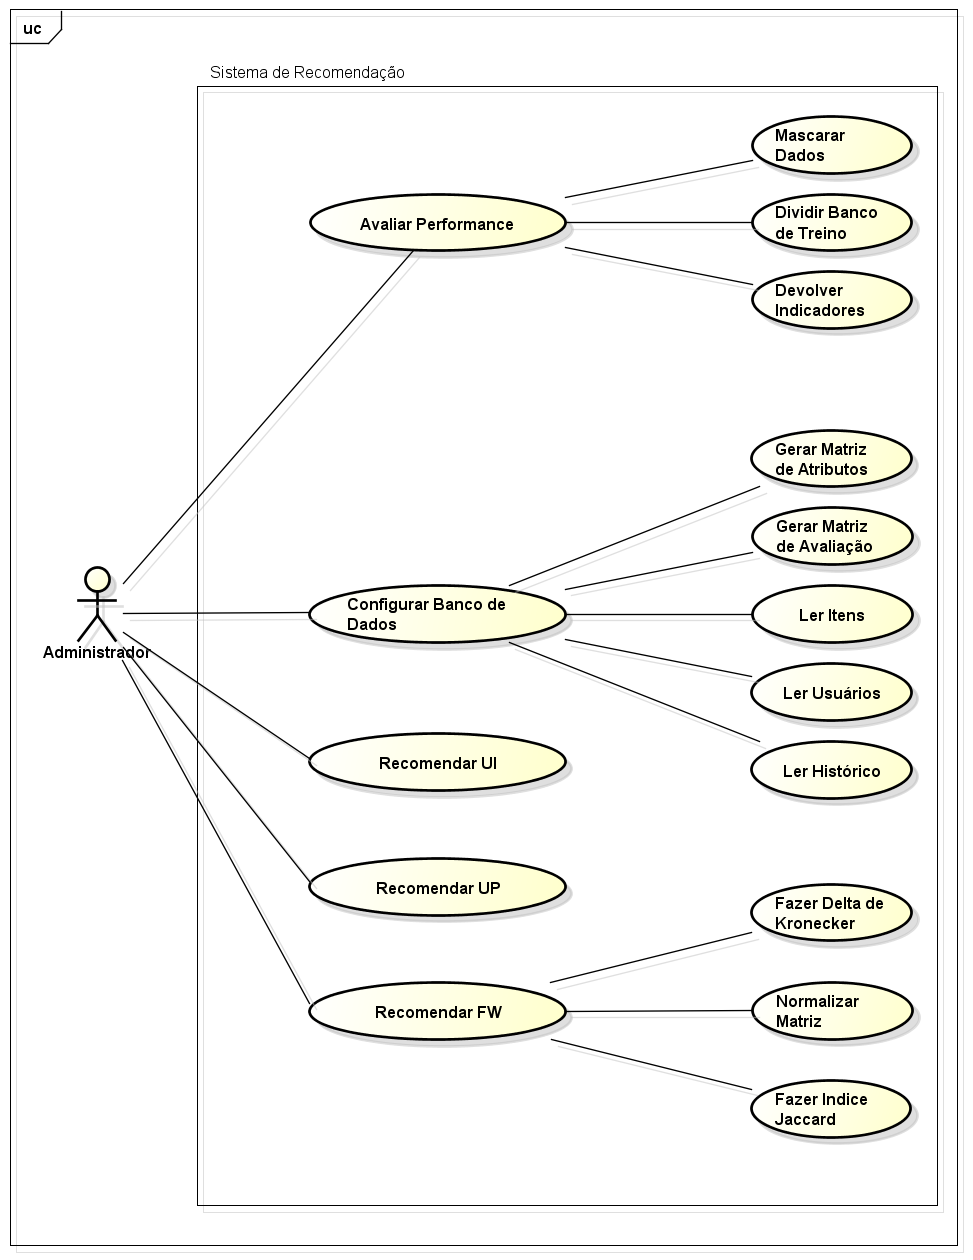
\includegraphics[width=0.9\textwidth]{img/CasosDeUso}
%    \end{center}
%\caption{Diagrama de Casos de Uso}
%\end{figure}
%\end{columns}
%\end{frame}
%
%
%\begin{frame}{Requisitos}{Diagrama de Casos de Uso - Avaliar Performance}
%
%\begin{figure}[ht]
%    \begin{center}
%    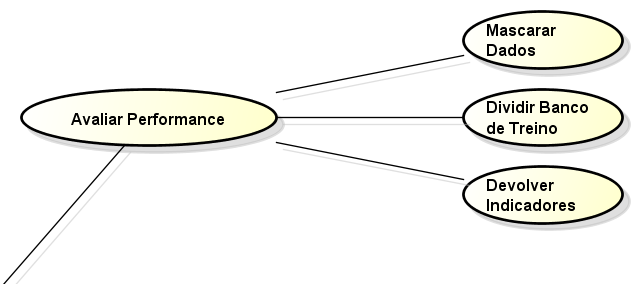
\includegraphics[width=0.9\textwidth]{img/CasosDeUso_Avaliar_Performance}
%    \end{center}
%\caption{Caso de Uso - Avaliar Performance}
%\end{figure}
%\end{frame}
%
%\begin{frame}{Requisitos}{Diagrama de Casos de Uso - Configurar Banco de Dados}
%
%\begin{figure}[ht]
%    \begin{center}
%    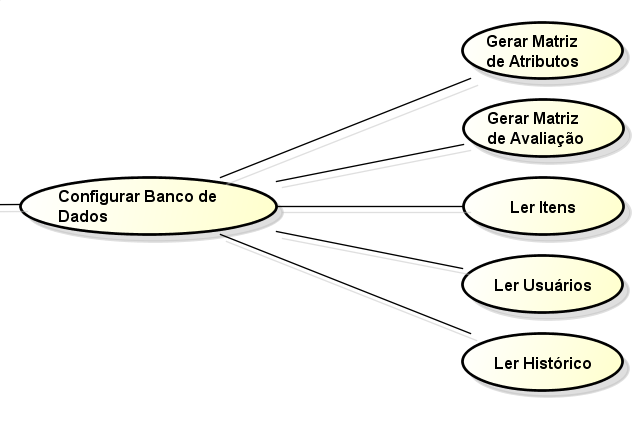
\includegraphics[width=0.9\textwidth]{img/CasosDeUso_Configurar_banco}
%    \end{center}
%\caption{Caso de Uso - Avaliar Performance}
%\end{figure}
%\end{frame}
%
%\begin{frame}{Requisitos}{Diagrama de Casos de Uso - Recomendar}
%
%\begin{figure}[ht]
%    \begin{center}
%    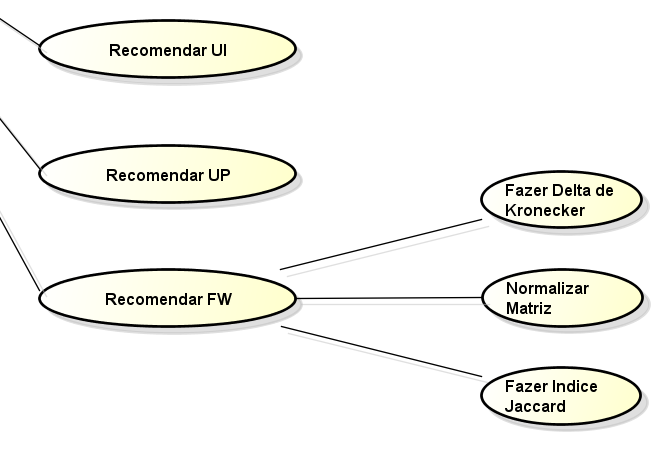
\includegraphics[width=0.9\textwidth]{img/CasosDeUso_Recomendar}
%    \end{center}
%\caption{Caso de Uso - Recomendar}
%\end{figure}
%\end{frame}
%!TEX root = index.tex

\chapter{Metodologia}

Será apresentado nesse capítulo a proposta de metodologia utilizada pelo autor para desenvolver o presente trabalho. Em primeira instância,  o objeto de estudo é apresentado, assim com as entidades associadas a ele. Posteriormente, são apresentadas as bases teóricas dos principais modelos analíticos utilizados na realização deste trabalho, de forma a esclarecer dúvidas quanto a sua utilização dentro do método apresentado. Por fim, a metodologia é esquematizada para ilustrar o alinhamento com os objetivos inicialmente definidos.

\section{Objeto de Estudo}

De forma a se aproximar de um dos principais nichos de seu interesse, a Samsung criou um programa de Relacionamento com Desenvolvedores, de forma a se aproximar de um grupo de profissionais que mais contribuem com a disseminação de novas tecnologias da Samsung. Esse programa possui diversas frentes, como o \textit{Developer Day}, que é um grande evento realizado uma vez por ano no Brasil e outros países da América Latina que visa promover as mais recentes tecnologias da marca, e o Laboratório Ocean, que visa a aproximação da comunidade estudantil e de startups em formação.

O Laboratório Ocean é uma iniciativa da Samsung que consiste em estimular desenvolvedores a criar soluções tecnológicas relacionadas aos produtos da marca coreana. A primeira sede do laboratório foi inaugurada em 2010 na Coréia do Sul, e a iniciativa foi replicada no Brasil há cerca de dois anos, com uma unidade em Manaus e outra em São Paulo. Ao passo que a unidade de Manaus foi estabelecida dentro da Universidade Estadual do Amazonas (UEA), a unidade de São Paulo encontrava-se até o fim de 2015 na Avenida Brigadeiro Faria Lima, uma das principais avenidas comerciais da cidade. Uma iniciativa recente movida por um ex-aluno, professores do departamento e o programa 'Parceiros da Poli' trouxe através de conversas informais a ideia de trazer o laboratório para dentro da USP. Como o modelo intra universitário funcionou bem em Manaus, foi decidido replicar o modelo e sediar o laboratório dentro da Universidade, hospedado dentro do Departamento de Engenharia de Produção (PRO).

O Ocean fornece dois tipos de cursos, básicos e intensivos. Os cursos básicos são de curta duração (aproximadamente 3 horas), e os cursos intensivos em seu módulo atual duram 4 meses, utilizando o espaço toda noite de segunda à quinta-feira. O foco inicial dos cursos foi o desenvolvimento em dispositivos móveis, em especial apoiados no sistema operacional Android, inerente aos aparelhos da Samsung, como o Galaxy S7. Com o passar do tempo, os cursos começaram a seguir as tendências de \textit{hardware} do mercado e consequentemente da própria Samsung, como \textit{wearables}, \textit{smart} TVs, Internet das Coisas e Realidade Virtual. Mesmo assim, a área de dispositivos móveis ainda representa 80\% dos cursos oferecidos por eles.

Os cursos curtos possuem como principal objetivo despertar o interesse de desenvolvedores em relação aos produtos da Samsung. Portanto, os cursos trabalham de forma a mostrar todos os produtos de alta tecnologia da samsung e capacitar desenvolvedores para que utilizem os seus dispositivos através do desenvolvimento de softwares. Para tal, é disseminado tanto o funcionamento dos \textit{Software Development Kits} (SDKs) da Samsung e suas APIs para permitir o acesso ao \textit{hardware} dos seus dispositivos quanto o uso do Android para manipulação do software na linguagem nativa atual do sistema operacional utilizado por eles. Para a execução desses cursos, a Samsung trabalha juntamente com empresas terceiras especialistas no assunto para preparar o material a ser passado. Algumas vezes funcionários da própria Samsung dão o treinamento, e em alguns momentos houve até participação do corpo docente da Poli.

Os cursos intensivos são cursos de pré-aceleração de empresas, e têm o intuito de fomentar o empreendedorismo, apesar de manter a base de disseminar o conhecimento em cima de produtos da Samsung. A empresa acredita que no atual mercado, a diferenciação competitiva sobre o \textit{hardware} está ficando cada vez mais difícil, por isso as empresas estão buscando se diferenciar frente às outras em conteúdo. Dentro desse contexto, a Samsung visa auxiliar empresas a se desenvolverem e elas - em contrapartida - auxiliam a enriquecer os produtos da Samsung, seja através de novos produtos ou através de serviços.

Dessa forma, os cursos de pré-aceleração procuram fornecer conhecimento e experiência ao desenvolvimento de suas empresas, através de mentorias, bate-papo, palestras e avaliações. Como são cursos gratuitos, um dos principais desafios é manter o próprio engajamento das empresas, por isso o motivo de haver encontros 4 vezes por semana, com mentoria, criação e gestão do projeto proposto pelo programa, com checkpoints de avaliação das empresas ao longo do projeto. Tudo isso feito de forma \textit{gamificada} dentro do próprio modelo. A primeira parte do programa consiste da validação do modelo de negócio proposto pela empresa, e a segunda parte corresponde à prototipação e desenvolvimento de produto de fato. Atualmente contribuem com esse programa os profissionais da Samsung, funcionários terceiros, professores da USP, membros do NEU e empresas parceiras (Sebrae, FIESP, IBM, Amazon).

A infraestrutura do laboratório consiste em uma grande sala para até 80 pessoas, porém caso necessário portas retráteis permitem a sua divisão em duas salas separadas. Essa estrutura fica aberta das 08 às 22 horas de segunda a sexta feira, podendo ser utilizada livremente pela comunidade estudantil da universidade, cedendo computadores e acesso a Wi-Fi de alta velocidade. As mesmas salas são utilizadas para a realização dos cursos mencionados anteriormente.

Por se tratar de um acordo entre a Samsung e o PRO, é necessário que sejam feitas reuniões de alinhamento das necessidades e expectativas entre partes, que não estão sendo realizadas nesse primeiro momento pois o projeto ainda está no início e não há conflitos aparentes. Entretanto a universidade também tem planos para o laboratório e acredita que o mesmo terá um grande impacto dentro e fora da universidade. Segundo as palavras do professor Eduardo Zancul na inauguração do Ocean: “É uma frente de ensino, pesquisa e extensão. Ensino pois será um espaço para disciplinas do curso de engenharia de produção; Pesquisa porque materiais e a estrutura do laboratório serão utilizados pela comunidade acadêmica; Extensão pois muitos cursos serão abertos para a comunidade”. O laboratório se tornou uma parceria de cogestão entre universidade e empresa que tem como principal mérito a geração de valor derivada da sinergia entre academia e indústria. 

\section{Análises Utilizadas}

Ao longo do desenvolvimento do trabalho encontrou-se a oportunidade de utilizar modelos analíticos que atendessem a duas principais necessidades encontradas pelo autor: 

\begin{enumerate}
\item Análise de grandes quantidades de dados qualitativos
\item Condensação e simplificação de dados de diversas fontes em um mesmo modelo
\end{enumerate} 

De forma a resolver o primeiro problema, a Análise de Conteúdo é um ótimo modelo pois confere a base teórica para a categorização de informações obtidas a partir de dados qualitativos de forma eficiente. Em relação ao segundo, foi encontrado no modelo de Análise SWOT um método muito ilustrativo, com uma simplicidade correspondente ao nível de extração de informação desejado, atuando também como um guia de identificação de pontos de análise e de balizador para a montagem das entrevistas.

\subsection{Análise de Conteúdo}
\label{cha:analise_conteudo}

Após a realização de uma pesquisa com um alto número de pessoas, um dos principais obstáculos do pesquisador é analisar um grande volume de dados em tempo hábil e eficaz em relação à absorção de informação do conteúdo apresentado. Em muitos casos, a falta de conhecimento de métodos de análise leva os analistas a lerem e relerem individualmente todas as respostas de forma a obterem uma interpretação mais profunda dos dados, porém além de a eficiência ser muito baixa, não significa que a interpretação dos resultados terá uma eficácia alta. De forma a sintetizar as informações presentes em mensagens escritas, orais ou qualquer outro meio de comunicação de forma eficaz, a análise de conteúdo permite unir a camada lógica da linguística com a semântica da hermenêutica para fazer essa tarefa.

A análise de conteúdo é um dos métodos mais utilizados para a avaliação de estudos qualitativos e consiste em um conjunto de técnicas de análise de comunicações que permitem encontrar os principais significados de um grande volume de mensagens, através de métodos lógicos e semânticos. Ela tem como principal técnica a inferência, que consiste em produzir suposições subliminares sobre determinadas mensagens, embasando-se em características da mensagem como o contexto em que é produzida ou recebida. \cite{bardin}

Um elemento interessante dessa metodologia é a sua capacidade de gerar tanto análises quantitativas quanto qualitativas, e até modelos híbridos se for de interesse da pesquisa. Como ela trata principalmente do sentido dos elementos presentes no conteúdo das mensagens, ela pode sugerir tanto uma contagem de frases e palavras quanto uma consideração do estado emocional dos comunicadores, e obter inferências acima do número de ocorrências no primeiro caso e uma análise subjetiva do contexto do segundo caso.

O método de análise do modelo de \citeonline{bardin} pode ser simplificado em quatro principais etapas:

\begin{figure}[h]
\caption{Etapas da análise de conteúdo}
\centerline{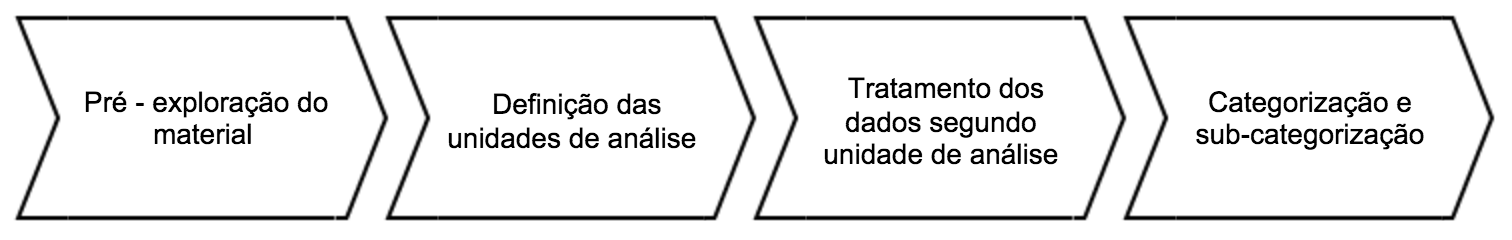
\includegraphics[scale=0.5]{img/fasesanalisedeconteudo}}
\label{fig:fasesanalisedeconteudo}
\caption* {Fonte: Simplificação do modelo \citeonline{bardin} realizada pelo autor}
\end{figure}

A fase inicial de pré-exploração tem como principal objetivo conhecer o contexto do material a ser analisado, retirar impressões e orientações para a próxima etapa. Um dos principais mecanismos dessa etapa é a leitura flutuante, que permite um primeiro contato com o conteúdo do "corpus de análise", raso o suficiente para gerar a formulação de algumas hipóteses e não tomar tempo excessivo do analista. A leitura menos aderente permite a assimilação do "corpus de análise" de forma não-estruturada permitindo a transcendência da mensagem de forma explícita para visualizar pistas não inicialmente óbvias.

Em seguida, é necessário definir a unidade de análise a ser trabalhada, baseada no conteúdo do material avaliado. Essas unidades podem incluir palavras, frases, parágrafos, textos inteiros, de tal forma que possa ser feito algum tipo de análise utilizando-as. A partir das inferências obtidas na etapa anterior, é possível que já tenha sido visualizado que tipo de análise ou categorização poderia ser feito posteriormente, dependendo do tipo de dado analisado. Quando há uma grande repetição de informação devido a um escopo fechado de cada mensagem, é possível utilizar palavras ou frases como unidade de análise para uma posterior análise frequencial. Para os casos em que há uma diversidade maior de informação, a utilização de trechos maiores de texto permitem uma análise temática, a fins de categorização posterior.

Como pode se tratar de um grande volume de dados, é possível que haja a necessidade de um tratamento desses dados de forma a chegar em representações condensadas e explicativas. Para textos maiores, seria oportuno coletar somente as partes relevantes que explicam o conteúdo da própria mensagem passada. Já para palavras e frases, é possível que ocorram palavras sinônimas e frases com o mesmo conteúdo semântico, que tratadas dentro de um mesmo contexto facilitariam a sua categorização posterior. Dentro desse contexto, softwares simples de contagem de palavras até outros mais complexos baseados em algoritmos de \textit{Machine Learning} ganham um espaço de atuação muito grande nessa área, por agilizar esse tipo de tratamento.

Finalmente, através do tratamento desses dados, é possível segmentar as unidades de análise em categorias e em sub-categorias, se necessário. O nível de granularidade ou o gênero dessas categorias deve variar segundo os pontos que querem ser abordados na análise, entretanto recomenda-se fazer a categorização em um nível mais granular, para poder ser feita uma recategorização em níveis menos granulares posteriormente, se necessário.

\subsection{Análise SWOT}
\label{cha:analise_swot}

A análise SWOT é uma ferramenta utilizada para analisar o ambiente e o contexto em que uma empresa se encontra posicionada diante do mercado. O processo de utilização consiste basicamente em organizar características da empresa e do ambiente em que se encontra em quatro principais avaliações: Pontos Fortes (\textit{Strengths}), Pontos Fracos (\textit{Weaknesses}), Oportunidades (\textit{Opportunities}) e Ameaças (\textit{Threats}), conforme quadro ilustrado abaixo. Essa modalidade de análise tem como principal vantagem a simplificação de uma estrutura complexa apresentada por uma organização, facilitando na tomada de decisões estratégicas.

\begin{figure}[H]
\caption{Quadro SWOT básico}
\centerline{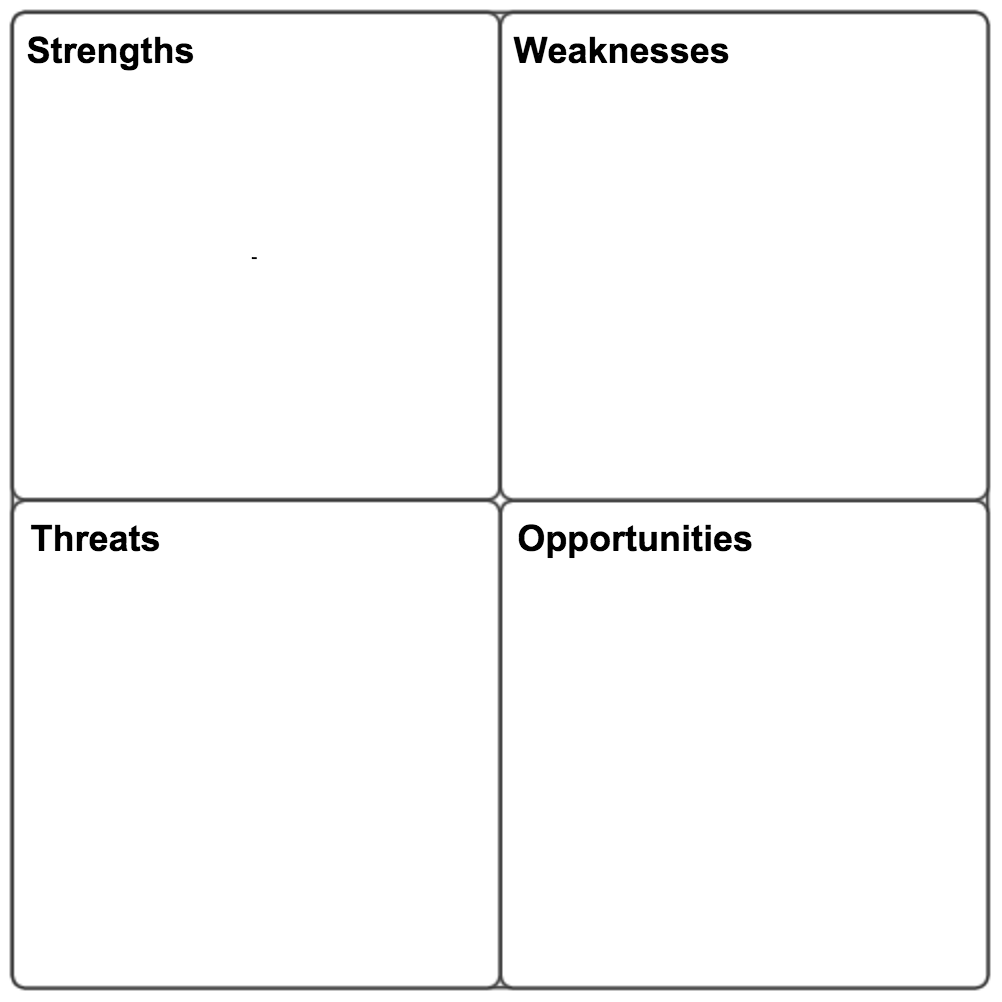
\includegraphics[scale=0.5]{img/detailedswot}}
\label{fig:detailedswot}
\caption* {Fonte: Quadro SWOT básico}
\end{figure}

\section{Método}

\label{chap:metodologia}

\begin{figure}[h]
\caption{Metodologia Utilizada no Trabalho}
\centerline{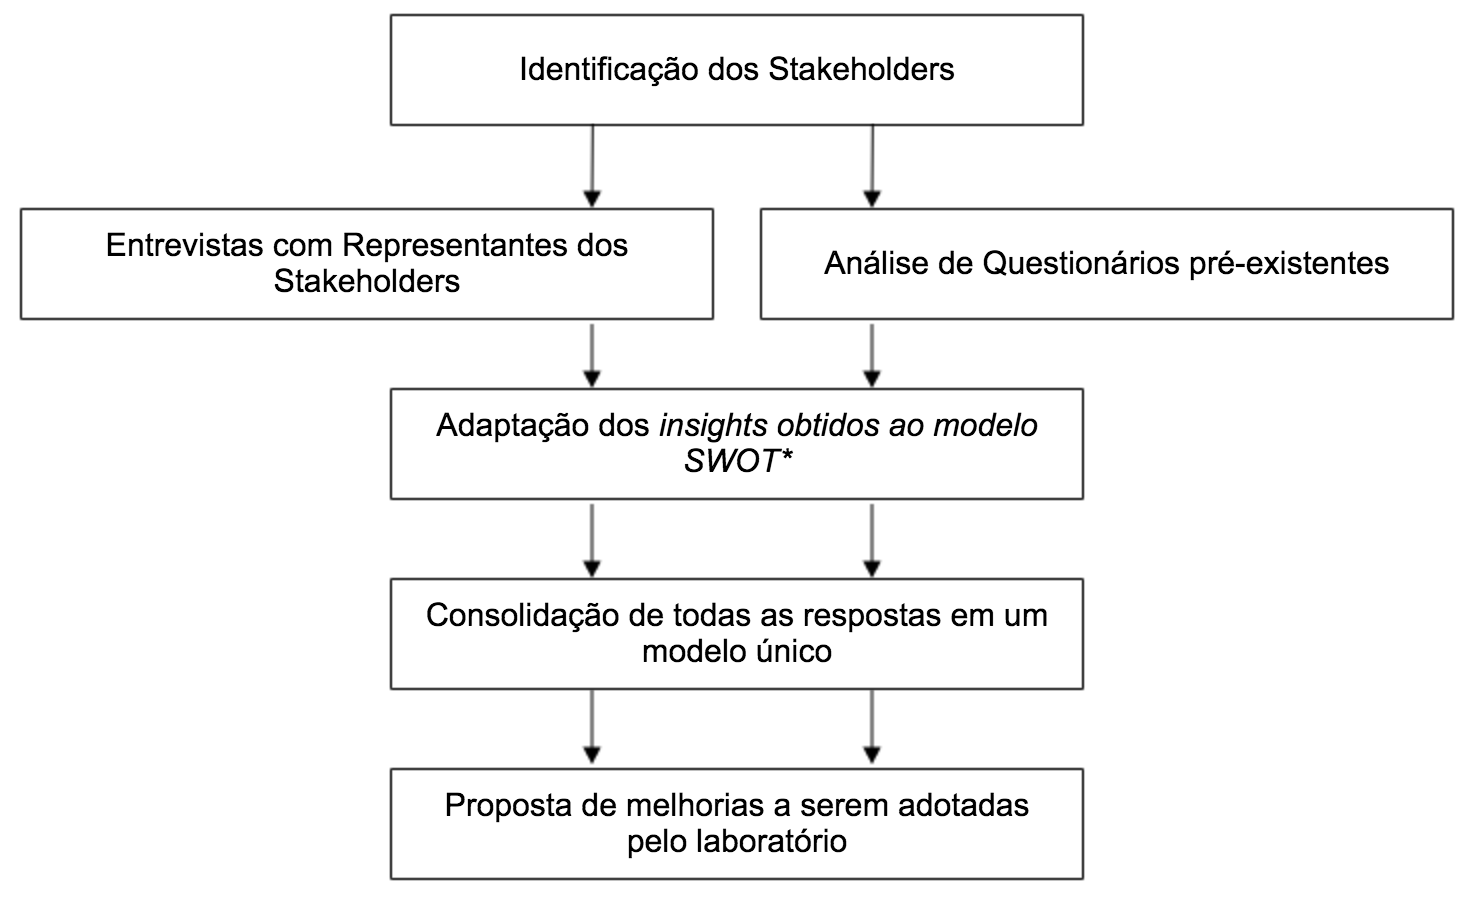
\includegraphics[scale=0.5]{img/metodologia}}
\label{fig:metodologia}
\caption* {Fonte: Elaborado pelo próprio autor}
\end{figure}

Após conversas iniciais com membros da Samsung e do PRO, foram definidos os stakeholders do projeto Ocean, juntamente com as pessoas-chave de cada. Foram realizadas entrevistas semi-estruturadas e gravadas, de forma a permitir a liberdade para serem feitas perguntas não presentes na estrutura inicial, e assim ter uma conversa guiada com o entrevistado como se não fosse uma entrevista formal. Antes de cada entrevista eram preparadas perguntas relacionadas ao mapeamento e percepção das interações do \textit{stakeholder} com o Ocean segundo a visão do entrevistador, e para todos os entrevistados era perguntado "se a pessoa teria alguma sugestão para a melhoria do Laboratório".

Para análise de um \textit{stakeholder} em particular, representado pelo alunos dos cursos básicos do programa Ocean que serão apresentados nesse capítulo, o método de entrevistas foi considerado menos eficiente pelo alto número e rotatividade de alunos. Juntamente a este fato, a Samsung tinha uma necessidade de analisar questionários de \textit{feedback} respondidos nos últimos dois anos de cursos, que nunca haviam sido analisados diante das suas questões qualitativas, apenas das quantitativas. Dessa forma, foram unidas as necessidades de ambas as partes e foram aproveitados esses questionários - totalizando um total de 5280 respostas - para extrair as informações necessárias para este trabalho. O modelo de questionário aplicado encontra-se em anexo. No caso, foram analisadas somente as respostas das questões analíticas: "O que mais o motivou nesse curso?", "O que você acha que pode ser melhorado?" e "Qual tema você gostaria que fosse abordado num próximo curso?".

De forma a analisar e extrair informações desses questionários, o autor optou por desenvolver um software próprio (https://github.com/GabrielArakaki/wordAnalysis) para manipular esses dados via palavras-chave, pelos motivos elencados a seguir.

\begin{description}
\item [Volume de Dados] A quantidade de dados é grande o suficiente para dificultar - porém não inviabilizar - a leitura individual de cada uma das respostas. Acredita-se que mesmo que se optasse pela leitura individual, ela deveria ser acompanhada de uma \textit{clusterização} das respostas em categorias, o que a análise via repetição de palavras-chave também permite encontrar. Em contrapartida, os dados são suficientemente pequenos a ponto de não ser viável buscar alternativas  de \textit{Machine Learning} existentes para tratar esses dados, pois o volume não seria suficiente para treinar a inteligência artificial utilizada.

\item [Proposta do Estudo] Embora exista um campo muito grande de possibilidades de tratar e manipular os dados presentes, existe a necessidade de seguir com os objetivos inicias do presente estudo, que diz respeito ao estudo do projeto Ocean de forma holística, e não somente na questão do aprendizado transmitido através de seus cursos. O autor acredita que há espaço para análises mais sofisticadas - dignas de um trabalho dedicado somente a isso - que poderiam ser realizadas caso a Samsung encontre a necessidade de entender os cursistas nos mínimos detalhes.

\item [Manipulação de Dados] O uso de uma ferramenta própria dá ao autor a liberdade de trabalhar e iterar em cima dos dados de forma a otimizar a ferramenta para o próprio uso. Existem disponíveis ferramentas prontas de geração de nuvens de palavras, que possuem um intuito muito maior de apresentar um 'choque visual' do que apresentar dados analíticos em si. A manipulação de dados permite que o autor encontre associações entre palavras ao observar os dados gerados pela ferramenta e trabalhar em cima da própria ferramenta para eliminar redundâncias ou dados inconsistentes.

\item [Desenvolvimento Ágil] O desenvolvimento ágil é um \textit{framework} de desenvolvimento de software que possui o intuito de permitir o desenvolvimento em um curto período de tempo com um iterações feitas através da coleta de \textit{feedbacks} de forma rápida e sistemática. No caso deste trabalho, o autor não encontrou uma ferramenta que fornecesse customização e flexibilidade conforme suas necessidades, fazendo com que optasse por desenvolver um software próprio. Não obstante, é de satisfação do autor como desenvolvedor utilizar programação para resolver problemas reais.
 
\end{description}

Para consolidar a análise realizada para cada \textit{stakeholder}, foi utilizada uma adaptação do modelo SWOT para ilustrar as percepções obtidas de cada um. Ela difere do modelo original do SWOT por não se tratar de uma análise de negócio baseada em fatores de mercado e competitividade com outros \textit{players}, e sim em uma análise fria e absoluta de fatores básicos em um projeto: Pontos Fortes, Pontos Fracos, Oportunidades e Ameaças. Foi considerado que por ser um modelo simples e de fácil visualização, consolidaria as necessidades deste trabalho sem desvirtuar os objetivos propostos.

A partir dos resultados obtidos pela análise das respostas, trabalhou-se em cima da geração de propostas de melhoria.

\section{Identificação de Stakeholders do Laboratório}
\label{sec:identificacao_stakeholders}

A partir de conversas informais com os professores mais próximos ao projeto Ocean e com os próprios responsáveis da Samsung pelo laboratório, foi possível desenhar um mapa ilustrativo para os principais \textit{stakeholders}.

\begin{figure}[H]
\caption{Mapa de stakeholders do projeto Ocean}
\centerline{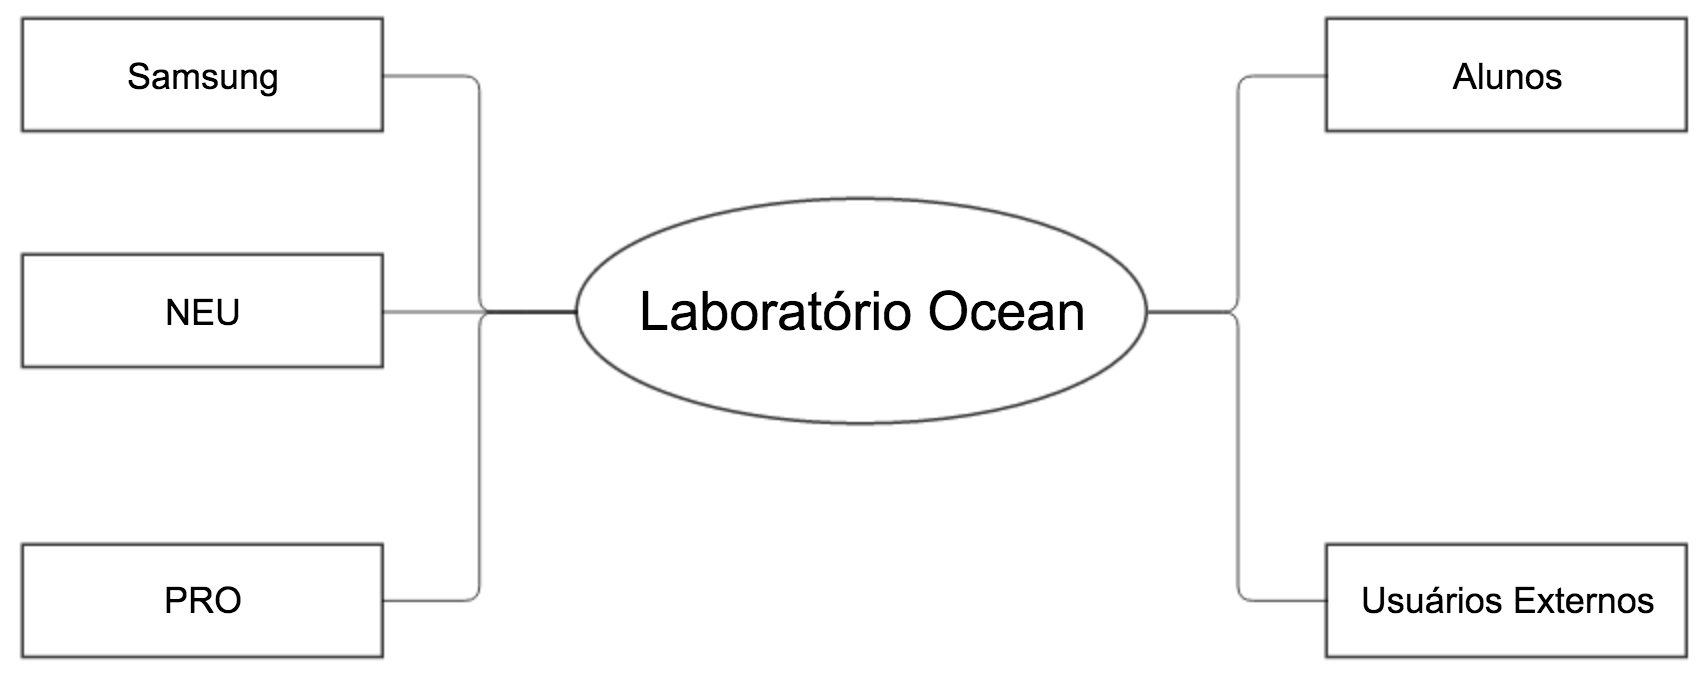
\includegraphics[scale=0.5]{img/stakeholders_v2}}
\label{fig:stakeholders}
\caption* {Fonte: Elaborado pelo próprio autor}
\end{figure}

Em um segundo momento foram definidos as principais fontes de dados para cada um dos \textit{stakeholders}, assim como os principais métodos de coleta, sendo definido o aproveitamento de questionários já respondidos pelos cursistas básicos e entrevistas para os demais.

\begin{figure}[H]
\caption{Pontos de contato dos \textit{stakeholders}}
\centerline{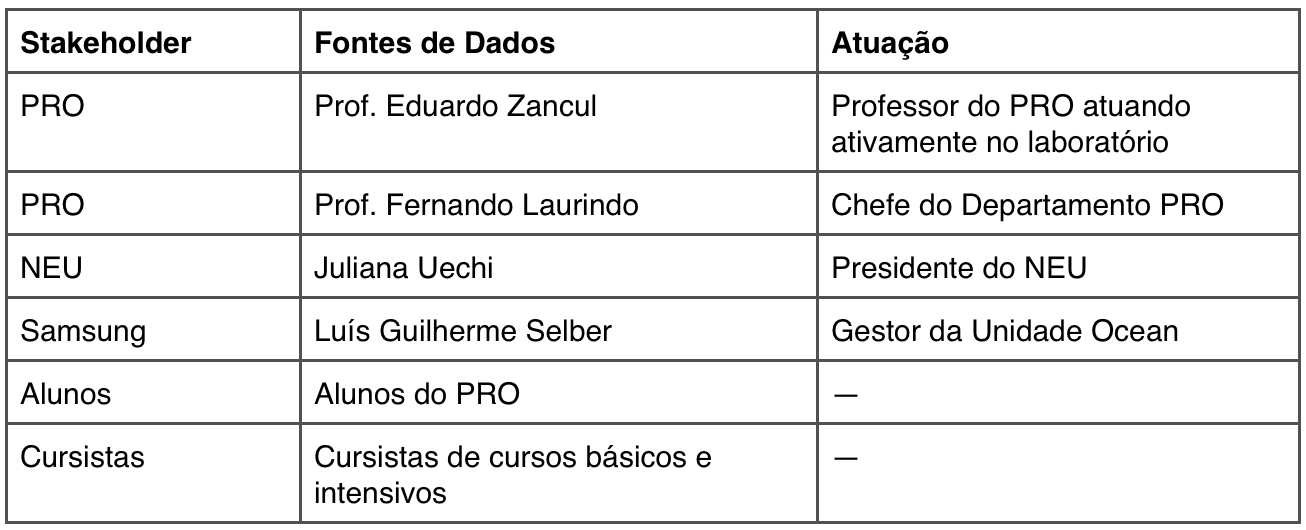
\includegraphics[scale=0.6]{img/stakeholderspoc}}
\label{fig:stakeholderspoc}
\caption* {Fonte: Elaborado pelo próprio autor}
\end{figure}


\subsection{PRO}
\label{sec:con_pro}

O Ocean é um dos quatro grandes projetos que o PRO acompanha atualmente, esquematizado pela Tabela \ref{tab:pilares_pro}, juntamente com Inovalab, a Fábrica Didática e o Núcleo de Empreendedorismo da USP.

\begin{table}[H]
\begin{center}
\caption{Pilares do PRO}
\label{tab:pilares_pro}
{\def\arraystretch{2}\tabcolsep=10pt
\begin{tabular}{>{\raggedright}p{0.2\linewidth}>{\raggedright\arraybackslash}p{0.2\linewidth}>{\raggedright\arraybackslash}p{0.2\linewidth}>{\raggedright\arraybackslash}p{0.2\linewidth}}
\hline
     & Objetivo Institucional & Participação do PRO & Em Atividade  \\ \hline
     Inovalab & Laboratório de Inovação & Gestão Ativa & Sim  \\
     Fábrica Didática & Apropriação de conceitos de fábricas para aplicação no ensino & Em Desenvolvimento & Não \\
     Ocean & Laboratório de Desenvolvimento de Software & Cogestão com a Samsung & Sim \\
	 Núcleo de Empreendedorismo da USP & Disseminação da cultura empreendedora & Cede espaço físico & Sim \\ \hline
\end{tabular}%
}
\caption* {Fonte: Elaborado pelo autor em conversa com professores do departamento}
\end{center}
\end{table}

O Inovalab é um laboratório que oferece recursos para realização de projetos de engenharia, como \textit{software}, \textit{hardware}, impressoras 3D e oficinas mecânicas. A infraestrutura do laboratório é utilizada para sediar o NEU, outro dos projetos que será discutido adiante. Já a Fábrica Didática é um projeto que consiste na produção de peças e produtos com a perspectiva de gerar pesquisa na área de fabricação e ensino para os alunos da engenharia de produção.

O que pode se ver em comum entre esses projetos e o Ocean é a proximidade da inovação e do empreendedorismo, pontos que o PRO considera essenciais para a tríade pesquisa, ensino e extensão. A Engenharia de Produção na Poli propicia um ambiente de aprendizado com disciplinas que já contribuem nessa área, como Projeto Integrado e Desenvolvimento de Produto, porém grande parte do aprendizado pode ser obtido através de atividades extra curriculares, propiciadas em parte por esses projetos. Um dos principais métodos de aprendizagem que a Poli incentiva nos alunos é o \textit{self-learning}, pois a área de Engenharia cobre uma variedade tão extensa de temas que o aluno que tiver interesse em se aprofundar em temas específicos deve buscar conhecimento por conta própria, sendo o principal papel da faculdade fornecer uma base sólida e uma estrutura para que ele possa adquirir conhecimento com facilidade.

\subsection{NEU}
\label{sec:con_neu}

O Núcleo de Empreendedorismo da USP é uma organização formada por alunos de graduação e pós-graduação, pesquisadores e professores que possuem a missão de promover a cultura de empreendedorismo dentro da Universidade. O NEU é aberto à toda comunidade da USP, já tendo recebido contribuições de diversas instituições da universidade, porém é formado atualmente principalmente por alunos da POLI e da FAU.

De forma similar ao estabelecimento do Ocean dentro do departamento do PRO, o NEU foi convidado a utilizar o espaço do Laboratório de Inovação (InovaLab) para sediar suas atividades. Atualmente o NEU trabalha com três principais pilares: inspiração, capacitação e conexão.

Inspiração diz respeito ao fomento ao empreendedorismo nos alunos para que eles se sintam impulsionados a participar do ecossistema de \textit{startups} ou até abrir as suas próprias. Portanto são feitos diversos convites aos diretores de diversas \textit{startups}, muitos com origens da própria USP, como Lean Survey, 99 Táxis e Squid, e estes podem explicar um pouco da sua trajetória e das emoções vividas graças aos seus empreendimentos. 

Capacitação é a frente do NEU de auxiliar ideias de alunos a se desenvolverem em produtos, para que assim sejam criadas novas empresas. A partir da rede de empresas que o NEU tem em seu leque de contatos, ele consegue encontrar mentorias para as empresas e acelerar o seu desenvolvimento. O principal programa dessa frente é o \textit{Startup Lab}, em que o NEU fornece material de apoio e mentoria através dos seus contatos com empresas, investidores e aceleradoras.

Conexão é representado principalmente pelo \textit{Startup Ship}, que é o canal do NEU destinado a alunos que querem estagiar em \textit{startups}. Através de sua rede de conexões ela facilita com que \textit{startups} e os alunos certos cheguem uns aos outros. Outro programa é o Pesquisas USP, que auxilia os alunos a se conectarem com pesquisas, e em contrapartida auxiliar pesquisadores a se conectarem com alunos ou empresas que possam auxiliar nos seus estudos. Nesse programa o NEU também auxilia startups a entrarem em contato com aceleradoras.

O NEU apresenta uma sinergia muito grande com o Ocean, pois ambos possuem muito interesse nessa fase de pré-aceleração de empresas, conseguindo exercer etapas distintas e complementares nesse processo. Durante os cursos intensivos do Ocean, o NEU se responsabiliza por trazer contatos de diferentes empresas para inspirar e fazer mentorias, ao passo que a Samsung trabalha fortemente na parte de capacitação e acompanhamento da evolução das empresas ao longo do programa.

Existe uma série de organismos dentro da universidade que fomentam a cultura de empreendedorismo, e como todos são gratuitos, existe uma colaboração muito grande para que os maiores beneficiados sejam as \textit{startups}, independente de  qual instituição que esteja contribuindo mais para a evolução da empresa.

\subsection{Alunos}
\label{sec:con_alunos}

A Engenharia de Produção é uma área que tem suas origens na engenharia mecânica, pois a formação de engenheiros no passado era voltada principalmente à capacitação técnica de produção de peças e produtos, sem um estudo aprofundado de como fabricá-los com eficiência. Os estudantes eram ensinados a desenhar um produto e desconstruí-lo em diversas peças que deveriam atuar conjuntamente para o funcionamento desejado. Encontrou-se então uma oportunidade de criar um novo ramo da Área Mecânica que se encarregaria de capacitar os alunos a aplicar conceitos de fábrica utilizados globalmente, como otimização das linhas de produção, controle da qualidade e controle da produção, não explorados anteriormente nos cursos de engenharia. Inicialmente voltado principalmente ao setor automotivo, a área de produção começou a ser expandida para poder aplicar os mesmos conceitos de fábrica para qualquer indústria, exigindo uma abstração dos principais conceitos, e inclusive a adoção de teorias de administração e gestão de projetos.

Atualmente, duas disciplinas eletivas estão utilizando a infraestrutura do laboratório, Desenvolvimento Integrado de Produto e Criação de Negócios Tecnológicos, porém o laboratório cede seu espaço a disciplinas que necessitem dos seus recursos. Muitas das reclamações dos alunos em relação ao ensino atual diz respeito às aulas que são passadas utilizando tecnologias antigas, como retroprojetores. Embora o laboratório não esteja sendo usado pelas disciplinas obrigatórios, os alunos enxergam que a sua presença eleva o patamar de tecnologia de ensino a ser utilizado, o que no curto ou médio prazo pode abandonar as tecnologias antigas para adotar o maior uso de mídias digitais.

Além da questão das disciplinas, o laboratório é utilizado pelos alunos durante o período fora da aula, para a realização de trabalhos , tarefas ou para fixar o conteúdo que foi dado em aula. Como o laboratório fica aberto até as 22 horas, e na cultura da engenharia é bastante comum ficar até tarde estudando, alunos utilizam o laboratório praticamente o dia inteiro. Antes do laboratório era frequente os alunos irem estudar em outros departamentos como a Engenharia Civil, que possui várias mesas no seu saguão principal, e ficava aberta até tarde para os alunos de pós-graduação. Embora grande parte dos alunos traz o seu próprio \textit{notebook} para estudar, alguns utilizam os notebooks da própria samsung e até um outro monitor para otimizar as suas tarefas.

A presença de um laboratório como este também ajuda a fomentar a cultura de empreendedorismo dentro da universidade, pois permite a capacitação dos alunos diante do desenvolvimento de produtos, base de criação de novas \textit{startups}. Segundo as pesquisas realizadas por \citeonline{entrepreneurship} com estudantes de graduação de engenharia, a experiência de empreendedorismo é observado de 4 maneiras, independentemente se eles desejam empreender ou não: 

\begin{enumerate}
\item Primeiro passo para o auto-aprendizado
\item Preparação para a vida no trabalho
\item Caminho para ser autônomo
\item Desenvolvimento de liderança e responsabilidade de um time
\end{enumerate}

Como esses pontos seguem na mesma direção dos objetivos da Poli e não agrada somente aqueles alunos que desejam ser empreendedores, o PRO pode continuar fomentando o empreendedorismo para que atinja todos os alunos. Entretanto, de forma a potencializar ainda mais os futuros empreendedores, é necessário entender o perfil daqueles alunos que desejam abrir o seu próprio negócio, como foi observado em diversas pesquisas como a realizada por \citeonline{empreendedorismo}, em que identifica o perfil de alunos que são atraídos pelo empreendedorismo:

\begin{itemize}
\item Propensão a assumir riscos
\item Proximidade a outros empreendedores no círculo próximo
\item Já possuem uma ideia desenvolvida para o empreendimento
\end{itemize}


\subsection{Cursistas}
\label{sec:con_cursistas}

Conforme explicado anteriormente, o Ocean trabalha com duas propostas de cursos, os cursos básicos e os cursos intensivos. O primeiro grupo corresponde à capacitação de desenvolvedores para que gerem conteúdo através de \textit{software} para dispositivos da Samsung, já o segundo é para pessoas que desejam empreender e possuem uma ideia inicial para ser desenvolvida. Embora exista uma gama de pessoas que seja usuária de ambos os cursos - os novos empreendedores têm muito interesse por programação - o público-alvo de cada um é diferente.

Os cursos básicos são desenhados para programadores ou aspirantes à programação. Embora existam diversos temas de cursos, o principal objetivo da Samsung consiste em capacitar os cursistas a explorarem todas as funcionalidades permitidas pelos \textit{hardwares} da Samsung. Para isso, são explorados o sistema operacional Android, os SDKs da Samsung, o sistema operacional Tizen, em suma tudo que possa contribuir para que o desenvolvedor possa gerar valor e conteúdo sem se preocupar em desenvolver um hardware específico. Portanto, é um curso de bastante interesse para iniciantes que desejam iniciar o aprendizado em programação, para desenvolvedores experientes que não tiveram muito contato com dispositivos móveis até para apaixonados pela Samsung que querem verificar na prática todo potencial permitido pelos seus dispositivos.

Segundo a 27\textsuperscript{a} Pesquisa de Anual do uso de TI, realizada pela Fundação Getúlio Vargas (FGV), o número de smartphones em uso no Brasil gira atualmente em torno de 168 milhões de dispositivos. \cite{tifgv}. Não obstante, além do alto número de smartphones, o Brasil também se mostra presente no mercado de outros dispositivos inteligentes, com previsão de movimentação de US\$4,1 bilhões no Brasil com IOT, segundo a assessoria de imprensa da IDC Brasil. \cite{idc}. Segundo a ONG Code.org, financiada por fundadores das maiores empresas de tecnologia do mundo como Mark Zuckerberg e Bill Gates, o número de empregos para programadores cresce exponencialmente, ao passo que o ensino de programação nas escolas não acompanha o mesmo ritmo, o que gerará uma falta de profissionais de TI em um futuro próximo. Juntamente a essa informação, o departamento de estatísticas de trabalho dos Estados Unidos (\textit{Bureau of Labor Statistics}) estima que o número de empregos para programadores fora dos EUA para trabalho remoto aumentará consideravelmente. \cite{bls}

É nesse cenário de alto crescimento do uso de novas tecnologias no Brasil que o mesmo se mostra como um grande mercado para produtos inerentes ao uso de dispositivos inteligentes, como aplicativos e games. Dentro desse contexto, jovens interessados pelo desenvolvimento desse mercado no país se interessam por propostas como a do Ocean para realizar diferentes cursos nessas áreas.
 
O segundo tipo de curso - cursos intensivos - foram feitos para incentivar ideias a se tornarem empresas, então é voltado para o nicho empreendedor. De acordo com o projeto \textit{Global Entrepreneurship Monitor}, que realiza pesquisas anuais sobre empreendedorismo no mundo, estima-se que em 2015, 52 milhões de brasileiros com idade entre 18 e 64 anos se envolveram na criação ou manutenção de algum negócio. Entre 2015 e 2014, houve um salto do total de empreendedores entre pessoas de 34,4\% para 39,9\% da população da faixa etária mencionada, principalmente devido ao surgimento de novas empresas. \cite{GEM}

Uma pequena parte dessas empresas é constituída de empresas com alto valor agregado e/ou com produtos de alta tecnologia, porém é visível o aumento da procura de pessoas que possuem ideias e buscam algum tipo de mentoria para desenvolvê-las a ponto de poder empreender. É nesse momento em que elas encontram o Ocean, onde podem utilizar de toda \textit{expertise} da Samsung para desenvolver um produto ou serviço de alta qualidade. Portanto não é necessário que os grupos já possuam uma empresa e um produto em funcionamento, até porque o programa desses cursos envolve questionar e validar hipóteses a respeito do próprio modelo de negócio da empresa, independente da maturidade da ideia. 

Os cursos intensivos são de uma extensão muito maior, e exigem uma intensidade muito grande dos cursistas, com reuniões de três horas de segunda à quinta-feira. Esse fator mostra a seriedade do programa em trabalhar com pessoas que mostrem um comprometimento acima da média, até porque muitos dos cursistas possuem emprego fixo e devem arranjar um tempo para se dedicar ao programa. Não obstante, além de ter esse acompanhamento quase diário nos dias úteis, são definidas metas semanais a serem cumpridas, para guiar as equipes no seu planejamento da semana. Toda essa intensidade tem o objetivo de deixar os alunos engajados ao longo do curso, que por ser gratuito e não exigir participação societária por parte da Samsung, pode facilmente ser abandonado se o aluno não observar o comprometimento da própria empresa.
%!TEX root = index.tex
\section[Síntese de Soluções]{Síntese de Soluções}
% subsubsection algoritmo_baseado_na_pondera_o_de_atributos_fw_ (end)
\begin{frame}{Síntese de Soluções}
\begin{alertblock}{Ponderação de Atributos (FW)}
$$
    s_{ij} = \sum_{f}{w_{f} \left(1-d_{fij}\right)}
$$
\end{alertblock}

\begin{block}{Perfil de Usuários (UP)}
$$
    s_{uv} = \frac{\sum\limits_{f \in \mathcal{F}_{uv}}{w_{uf}~w_{vf}}}{\sqrt{\sum\limits_{f \in \mathcal{F}_{uv}
    }w_{uf}^2} \sqrt{\sum\limits_{f \in \mathcal{F}_{uv}}w_{vf}^2}} 
$$
\end{block}

\begin{exampleblock}{Perfil Usuário-Item (UI)}
$$
    \omega_{ui} = \sum_{f}{w_{uf}~a_{if}}
$$
\end{exampleblock}


%\begin{table}[hp]
%\begin{center}
%    \caption{Medidas de distância entre alguns atributos}
%    \label{tab:medidas-distancia}
%    \begin{tabular}{  | p{3cm} | p{3cm} | p{3cm} | } 
%    \hline
%    \textbf{Atributo} $f$ & \textbf{Domínio} $\mathrm{F}$ & \textbf{Distância} $d_f$ \\ \hline
%    Marca & Literal & $1-\delta^f_{ij}$ \\ \hline    
%    Cor & $\left(\mathbb{N}\backslash \mathbb{N}_{256}\right)^3$  & $ \frac{\lVert a_{if}-a_{jf} \rVert_2}{\max_{i,j}{\lVert a_{if}-a_{jf} \rVert_2}} $ \\ \hline
%    Preço & $\mathbb{R}$ & $ \frac{\left| a_{if}-a_{jf} \right|}{\max_{i,j}{\left| a_{if}-a_{jf} \right|}} $ \\ \hline
%    \end{tabular}
%\end{center}
%\end{table}
\end{frame}





%%!TEX root = index.tex
\section[Biblioteca]{Biblioteca}
\begin{frame}{Biblioteca}{Ferramentas Utilizadas}

\textbf{IDE RStudio}
	\begin{itemize}
		\item Console
		\item Editor de texto e corretor de sintaxe
		\item Suporte a execução direta de código
		\item Visualização de gráficos
		\item Depuração de erros
		\item Gerenciamento de espaço de trabalho
	\end{itemize}
\end{frame}

\begin{frame}{Biblioteca}{Estrutura}
\textbf{Quatro principais seções}
\begin{description}
	\item DB
	\begin{itemize}
		\item Contém o banco de dados MovieLens 100k
	\end{itemize}
	\item Methods
	\begin{itemize}
		\item Contém os algoritmos de recomendação
	\end{itemize}
	\item Results
	\begin{itemize}
		\item Contém os métodos de avaliação de qualidade
	\end{itemize}
	\item Setup
	\begin{itemize}
		\item Contém funções de suporte
	\end{itemize}
\end{description}
\end{frame}

%%!TEX root = index.tex
\section[Avaliação de Desempenho]{Avaliação de Desempenho}
\begin{frame}{Avaliação de Desempenho}


\begin{itemize}
	\item Distância entre recomendações
	\begin{itemize}
		\item $EMA = \left|\hat{\textbf{\i}} - \textbf{i}\right|$
	\end{itemize}
	\item Desempenho mediante a mudança nas variáveis 
	\begin{itemize}
		\item Quantidade de atributos utilizados
	\end{itemize}
	\item Tempo de execução
	\begin{itemize}
		\item Em função do algoritmo
		\item Em função do tamanho do banco de dados
	\end{itemize}
\end{itemize}

\begin{table}[ht]
\begin{center}
    \label{tab:avaliacao-predicao}
    \caption{Avaliação de sistemas de predição}
    \begin{tabular}{  | p{2cm} | p{2.5cm} | p{4cm} | }
    \hline
    \textbf{Medida} & \textbf{Fórmula} & \textbf{Significado} \\ \hline
    Precisão &  $\frac{VP}{VP+FP}$ & \% Predições corretas de casos positivos \\ \hline                            
    Acurácia & $\frac{VP+VN}{VP+VN+FP+FN}$ & \% Predições corretas  \\ \hline
    \end{tabular}
\end{center}
\end{table}

\end{frame}


%!TEX root = index.tex
\section[Resultados]{Resultados}

\begin{frame}{Resultados}
\begin{table}[hp]
\begin{center}
    \caption{Parâmetros de influência no desempenho dos algoritmos de recomendação}\vspace{-.5cm}
    \label{tab:variaveis}
    \begin{tabular}{  | p{1.5cm} | p{5.5cm} | p{3.0cm} | } 
    \hline
    \textbf{Variável} & \textbf{Descrição} & \textbf{Valor padrão}  \\ \hline
    $N$ & Lista de recomendação & $20$ \\ \hline   
    $T$ & Base de treinamento & $75\%$ \\ \hline
    $H$ & Avaliações ``escondidas'' & $75\%$ \\ \hline
    $d^f$ & Medida de distância & Distância $L_1$~$\left|\left|\cdot\right|\right|^f$ \\ \hline
    $\mathcal{F}$ & Conjunto de atributos dos itens & Todos atributos \\ \hline
    $M$ & Avaliações positivas & $2$ \\ \hline
    $k$ & Vizinhos mais próximos & $10$ \\ \hline
    $W$ & Quantidade de pesos & Todo $w_f>0$ \\ \hline
    \end{tabular}
\end{center}
\end{table}
\end{frame}

\begin{frame}{Resultados}{Tamanho da lista de recomendação $N$}

\begin{columns}[b]
\column{.5\textwidth} %
\begin{figure}[ht]
    \begin{center}
    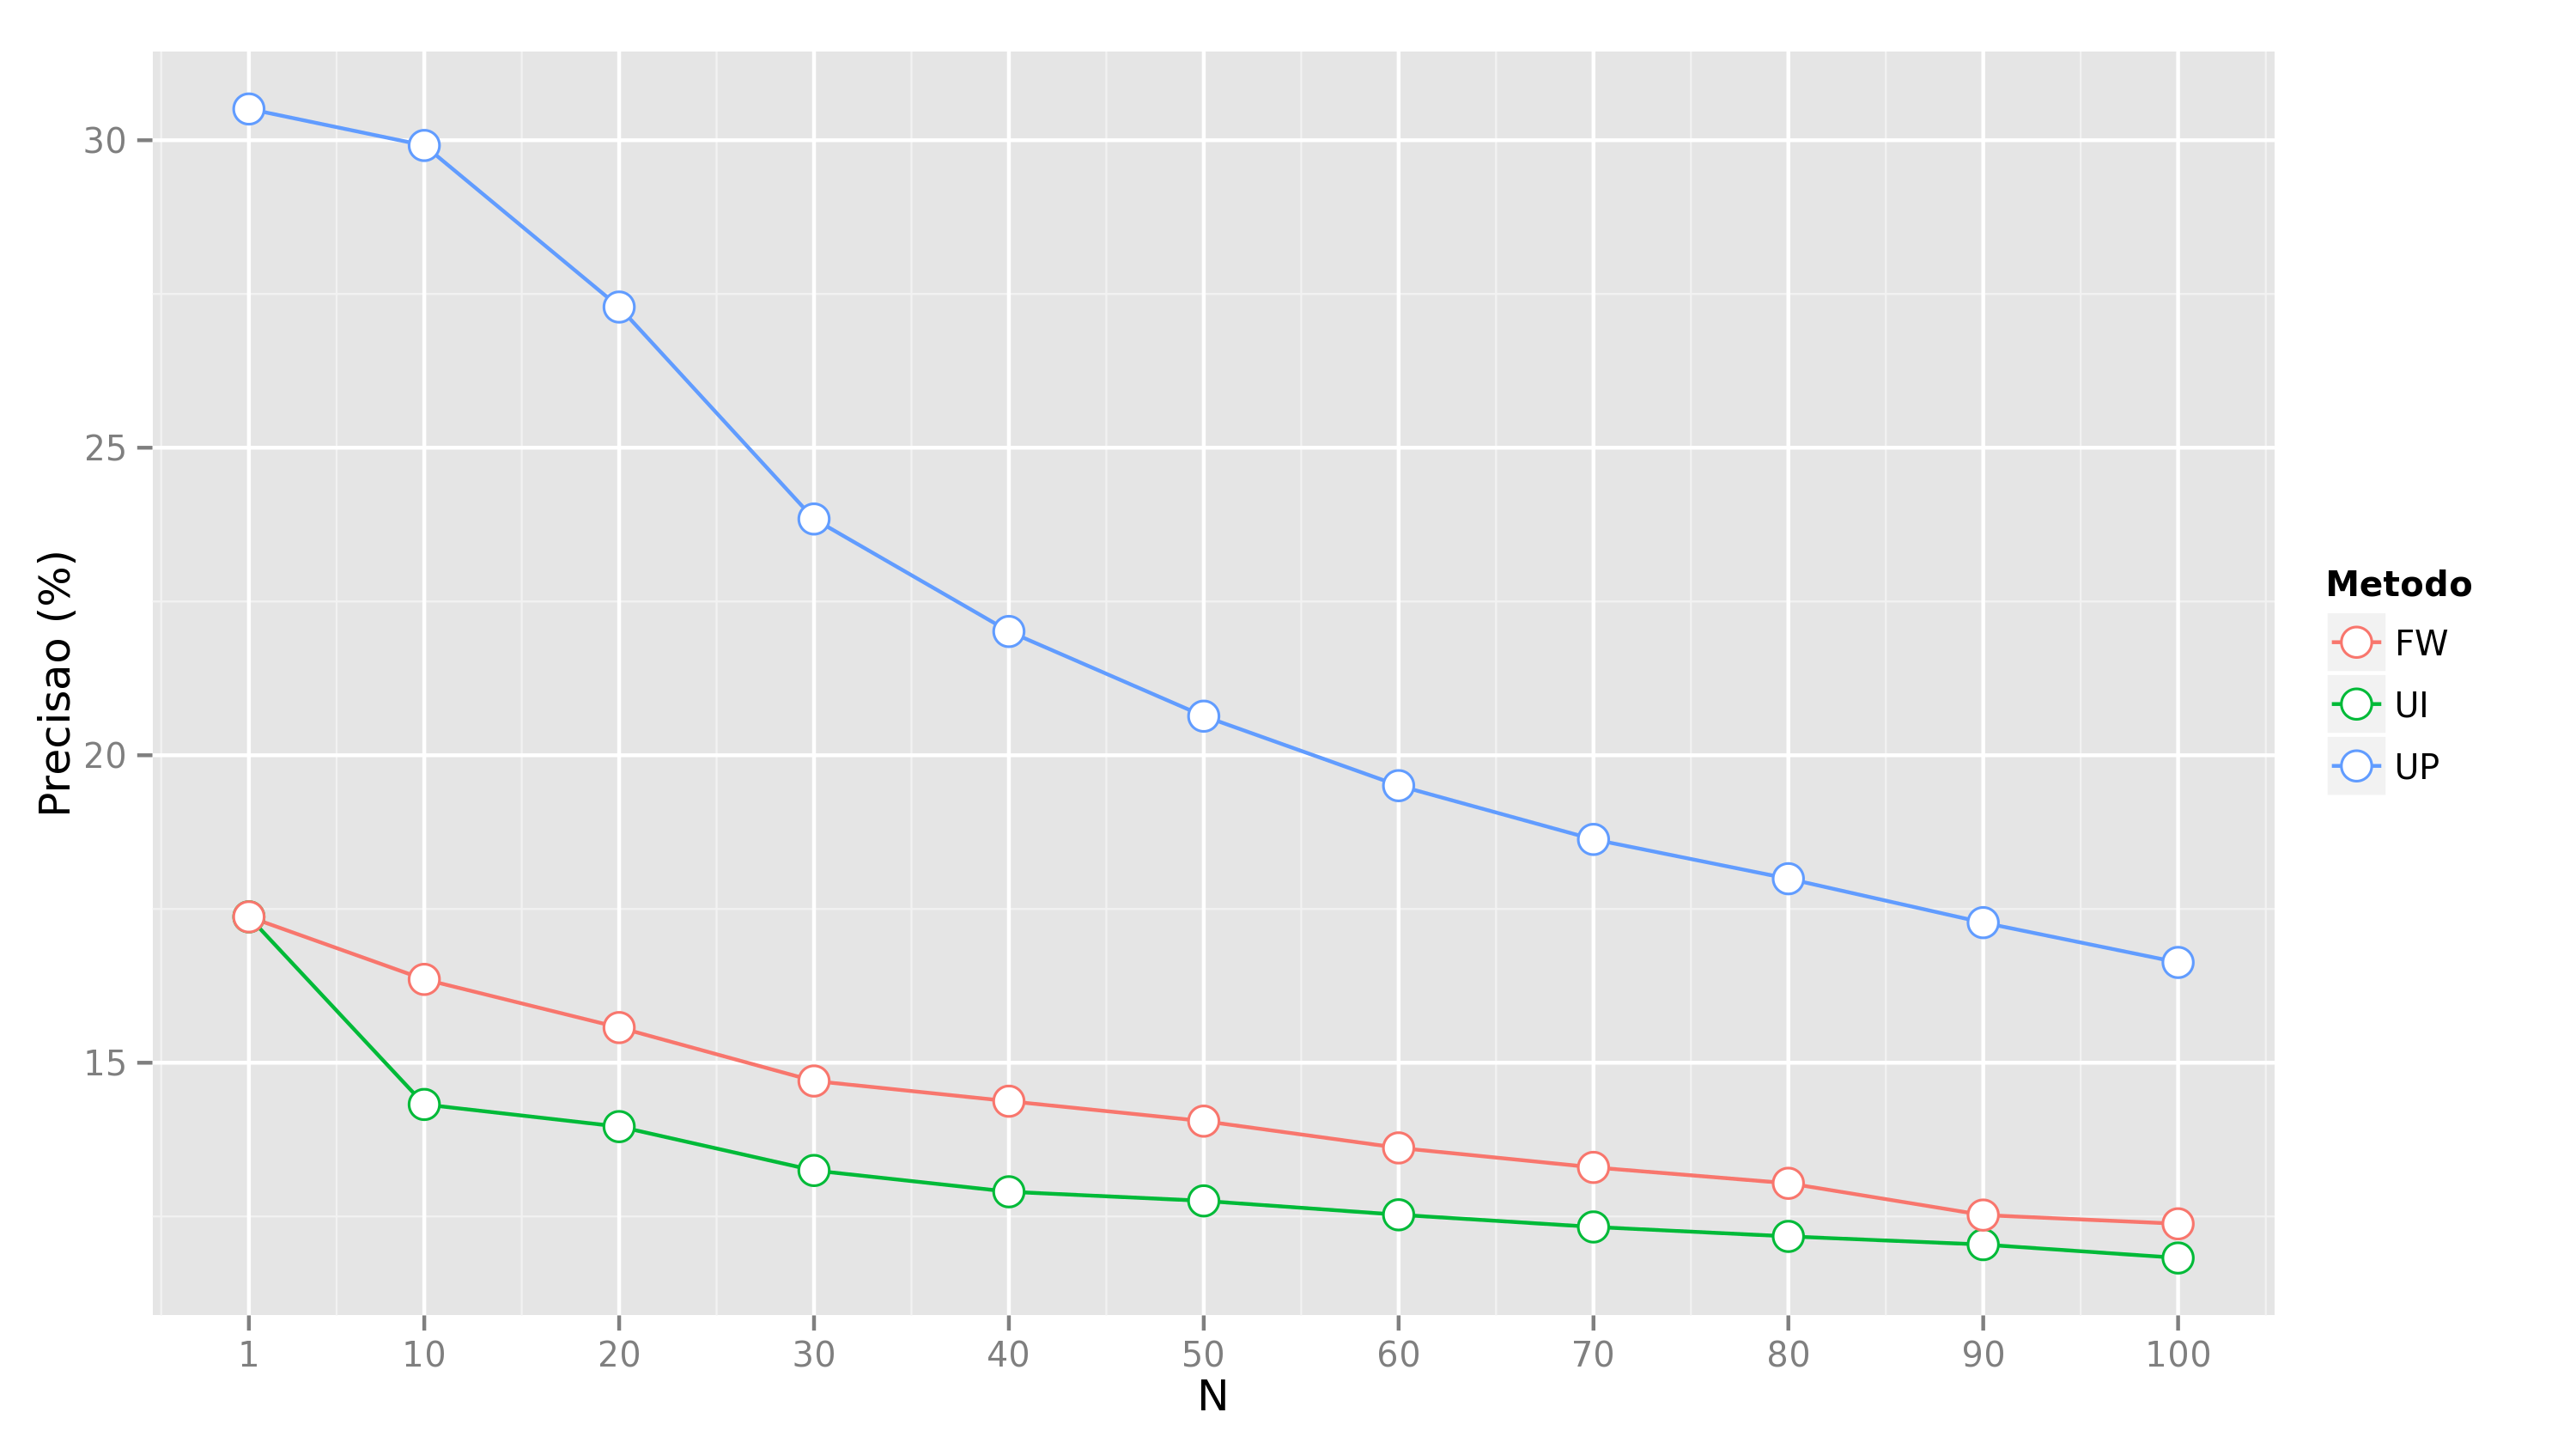
\includegraphics[width=1.1\textwidth]{../img/precision_N}
    \end{center}
    \caption{Precisão $\times$ $N$}
    \label{fig:precision_N}
\end{figure}

\column{.5\textwidth} % 

\begin{figure}[ht]
    \begin{center}
    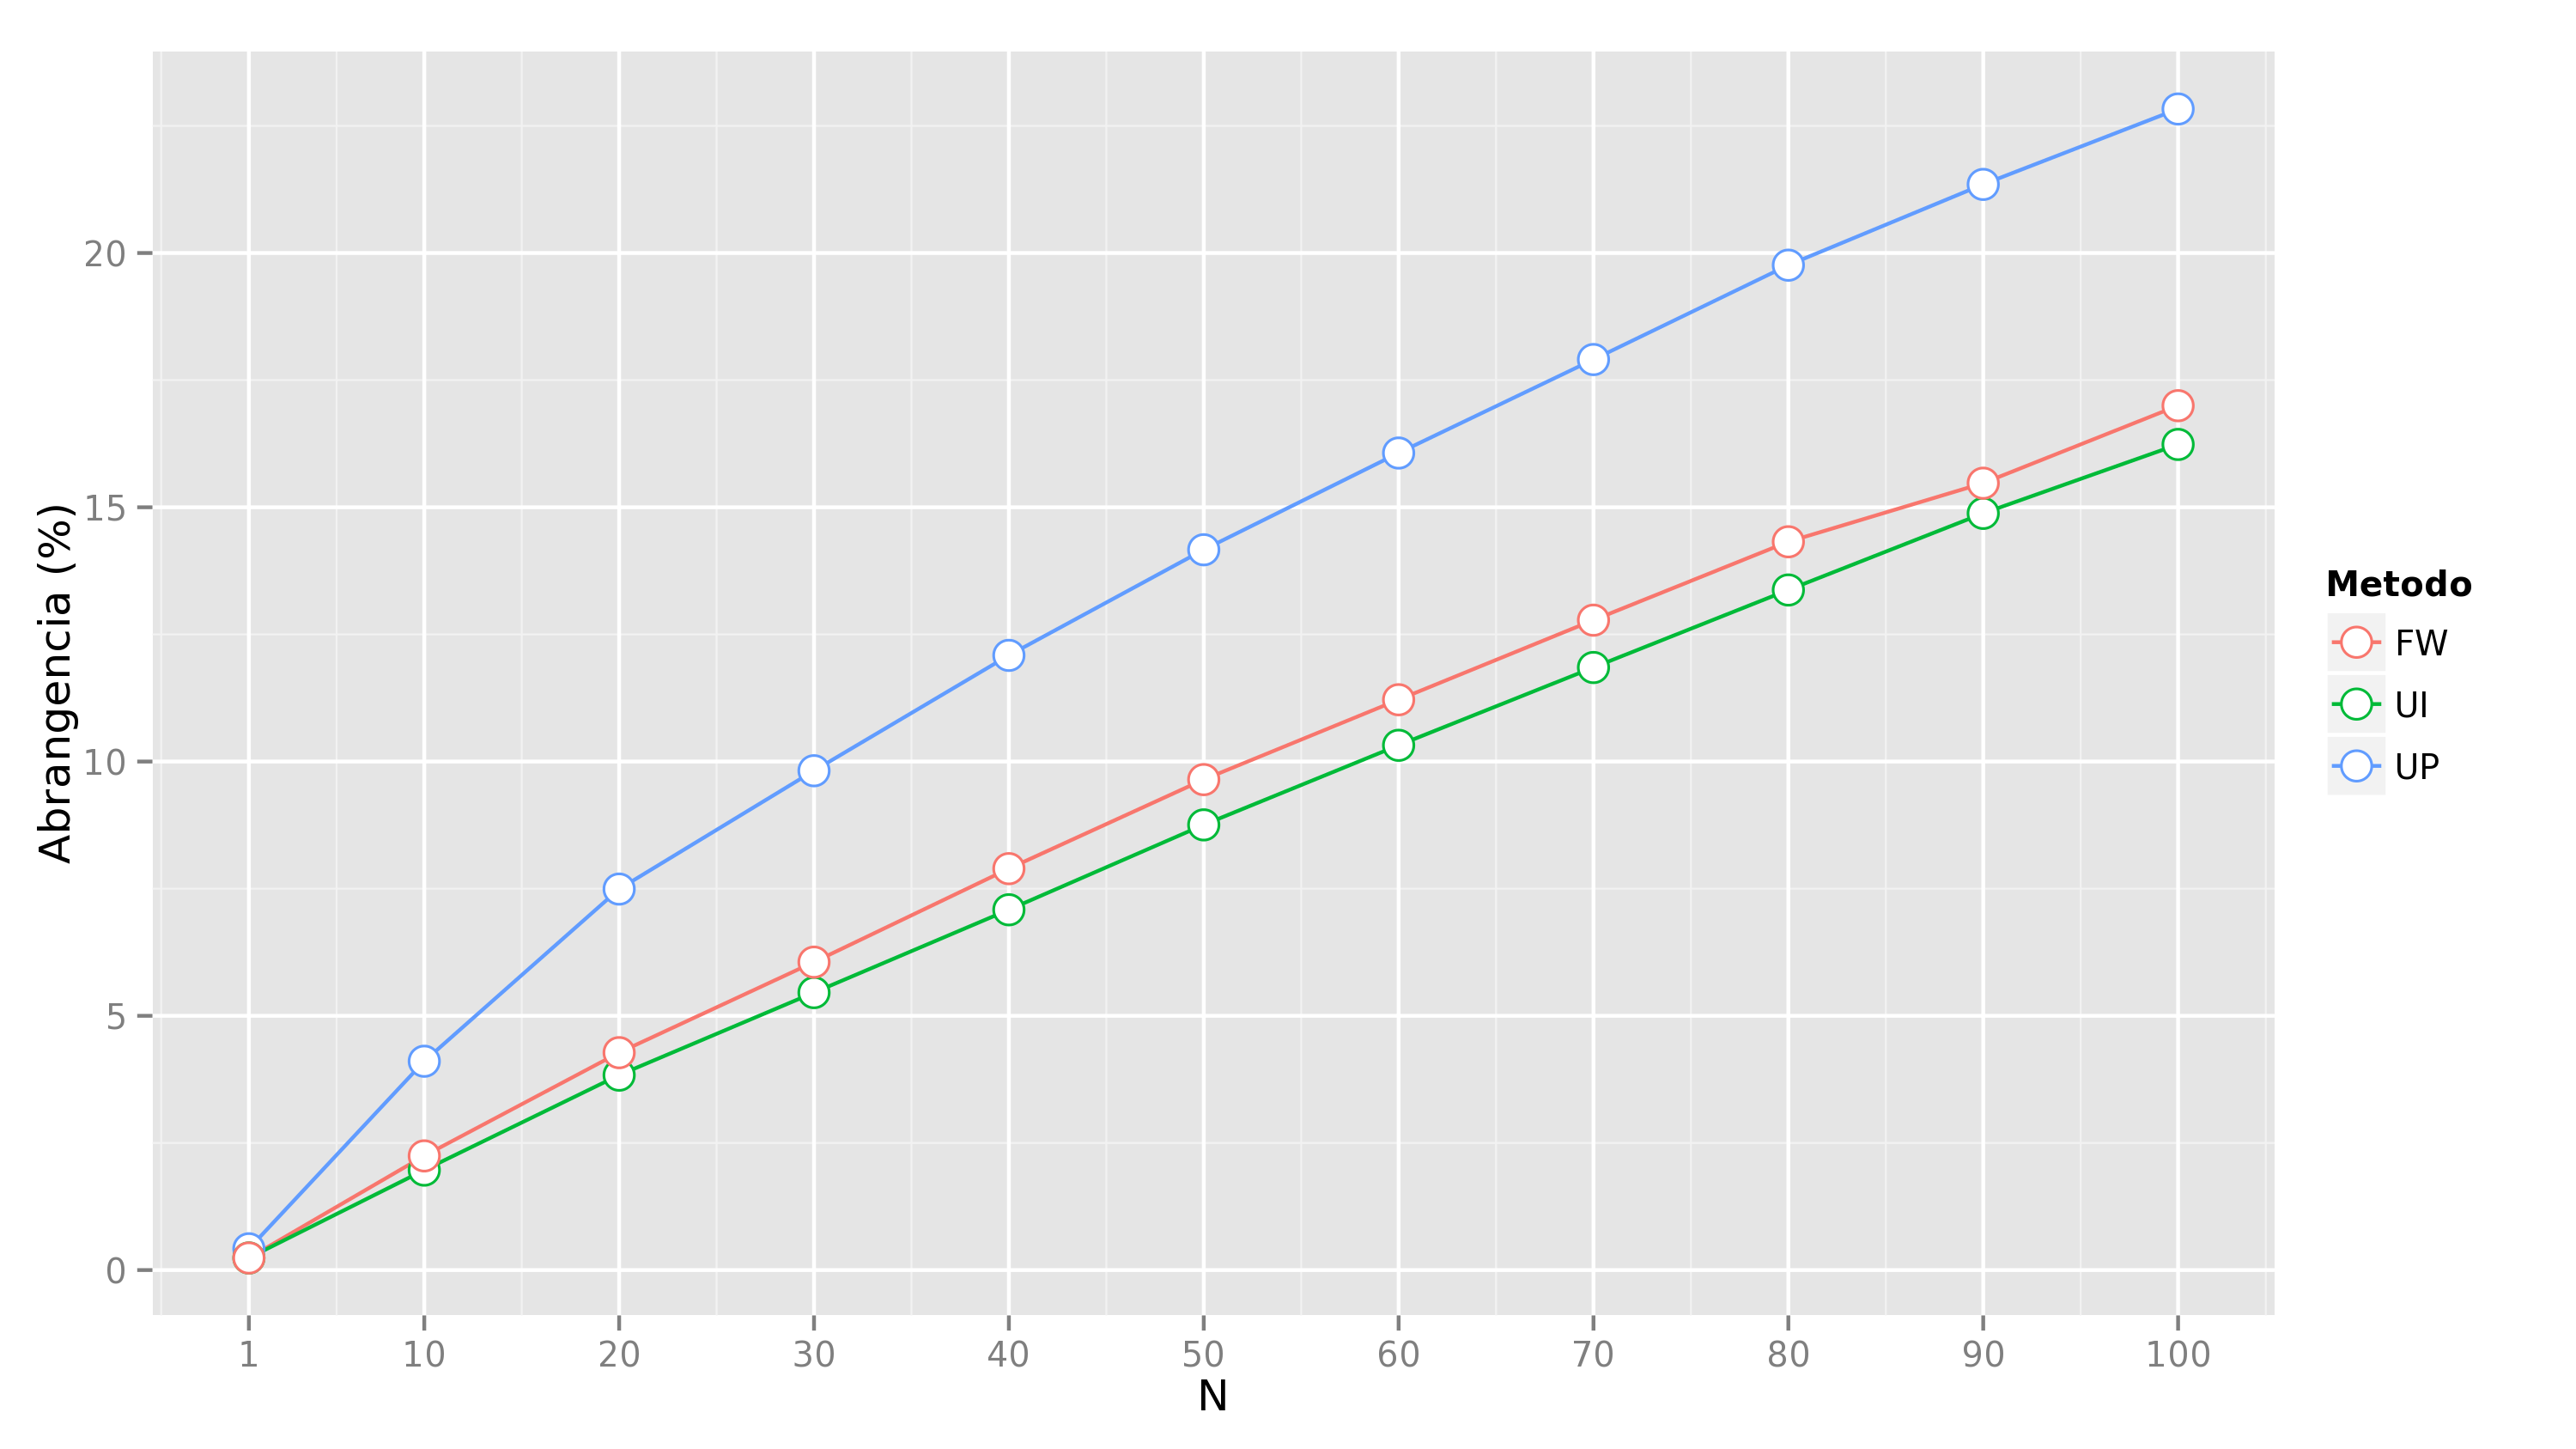
\includegraphics[width=1.1\textwidth]{../img/recall_N}
    \end{center}
    \caption{Abrangência $\times$ $N$}
    \label{fig:recall_N}
\end{figure}
\end{columns}
\end{frame}

\begin{frame}{Resultados}{Tamanho da lista de recomendação $N$}
\begin{columns}[b]
\column{.5\textwidth} %
\begin{figure}[ht]
    \begin{center}
    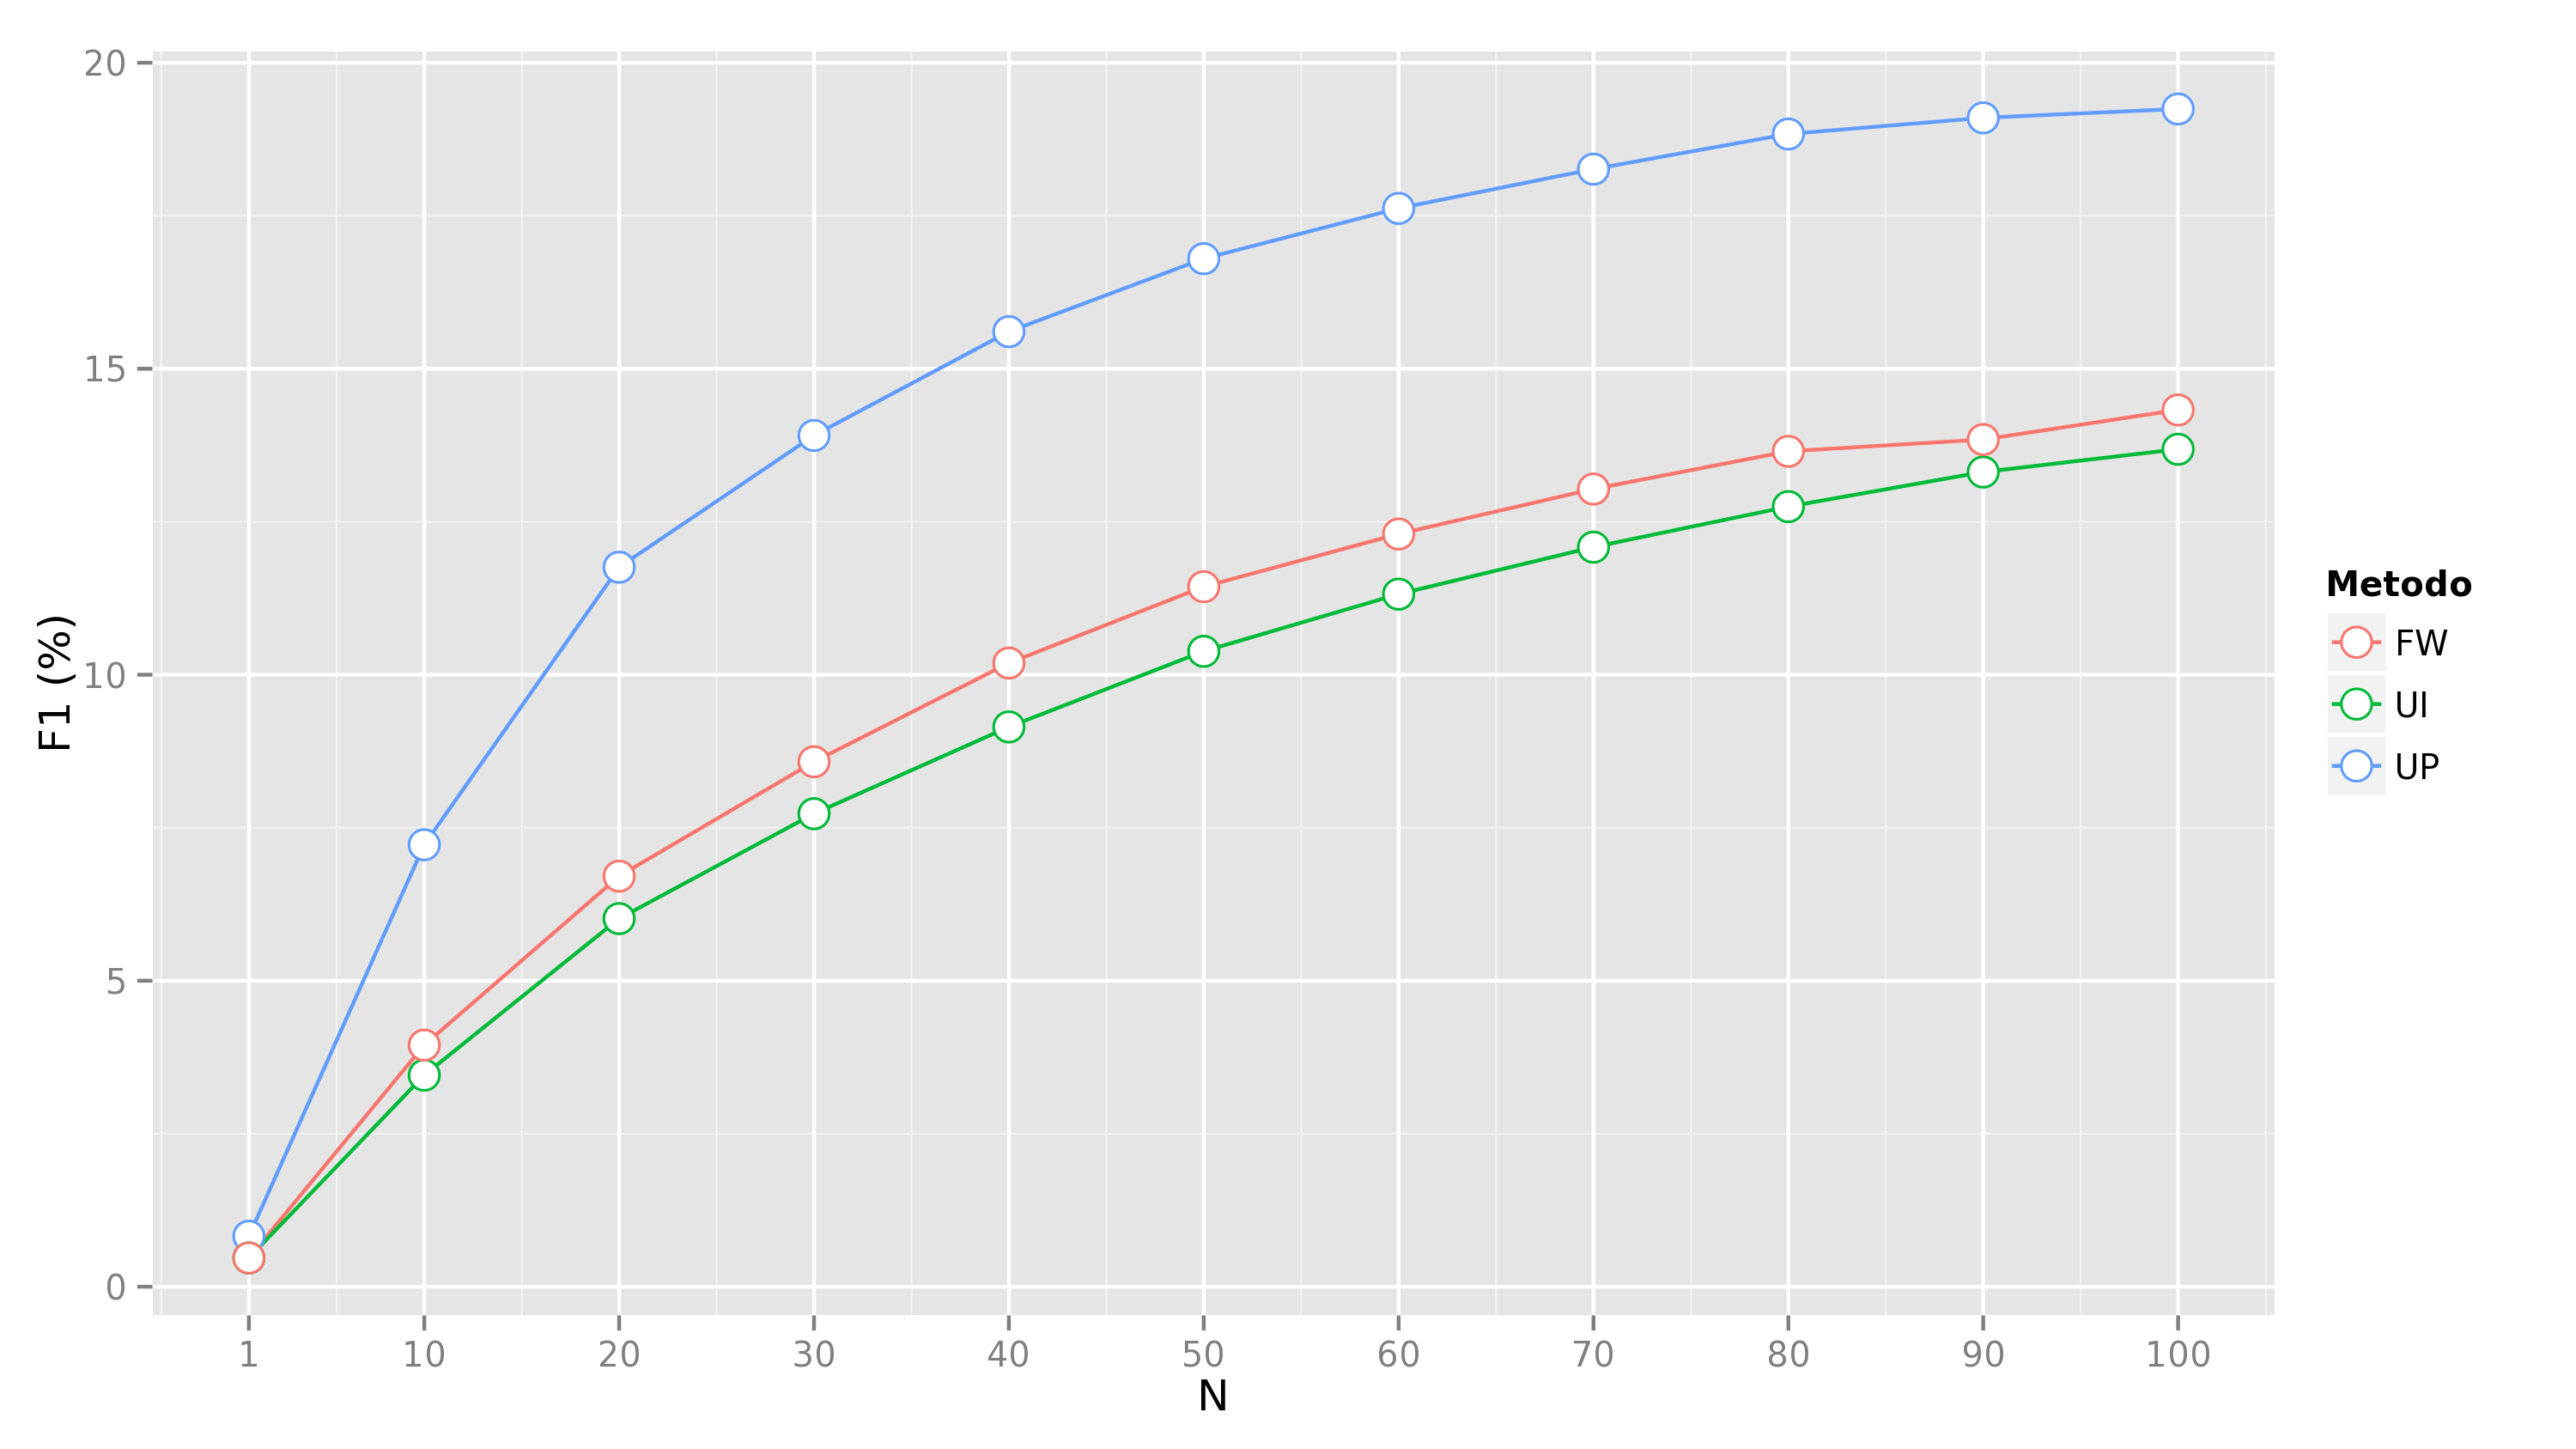
\includegraphics[width=1.1\textwidth]{../img/F1_N}
    \end{center}
    \caption{$F_1$ $\times$ $N$}
    \label{fig:F1_N}
\end{figure}

\column{.5\textwidth} % 

\begin{figure}[ht]
    \begin{center}
    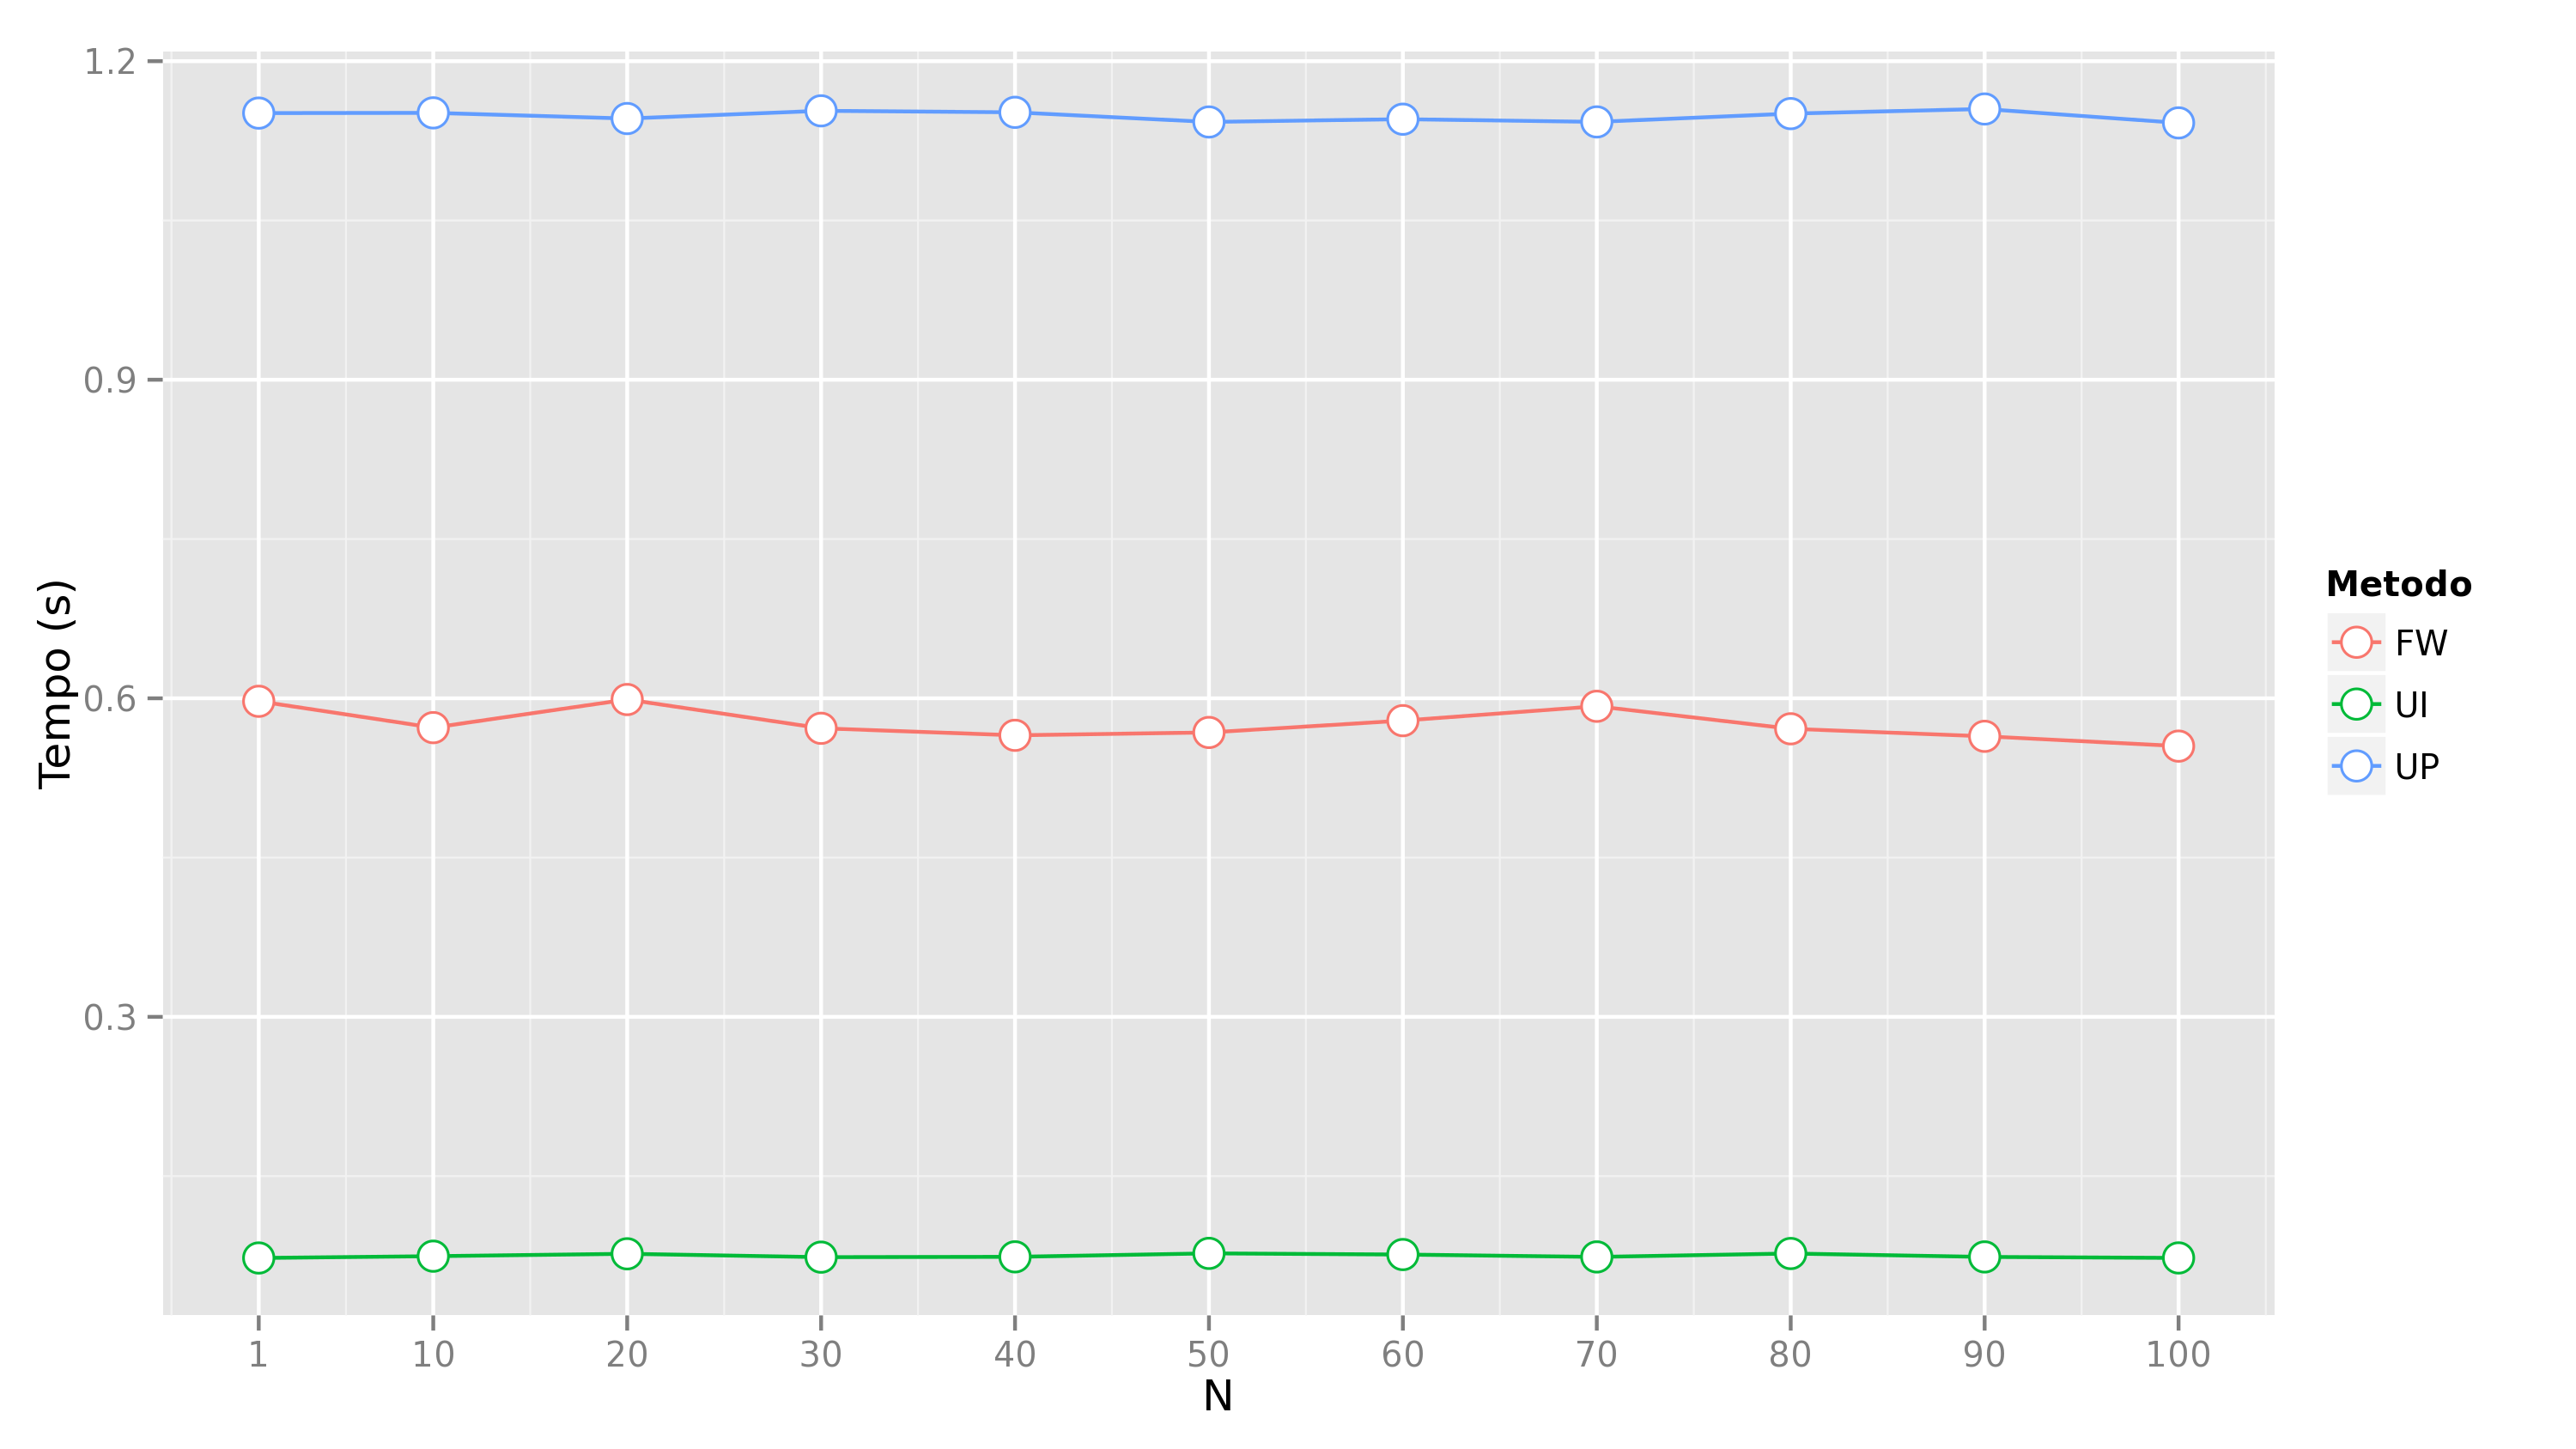
\includegraphics[width=1.1\textwidth]{../img/time_N}
    \end{center}
    \caption{Tempo $\times$ $N$}
    \label{fig:time_N}
\end{figure}
\end{columns}
\end{frame}

\begin{frame}{Resultados}{Percentual da base de aprendizado $T$}
\begin{figure}[ht]
    \begin{center}
    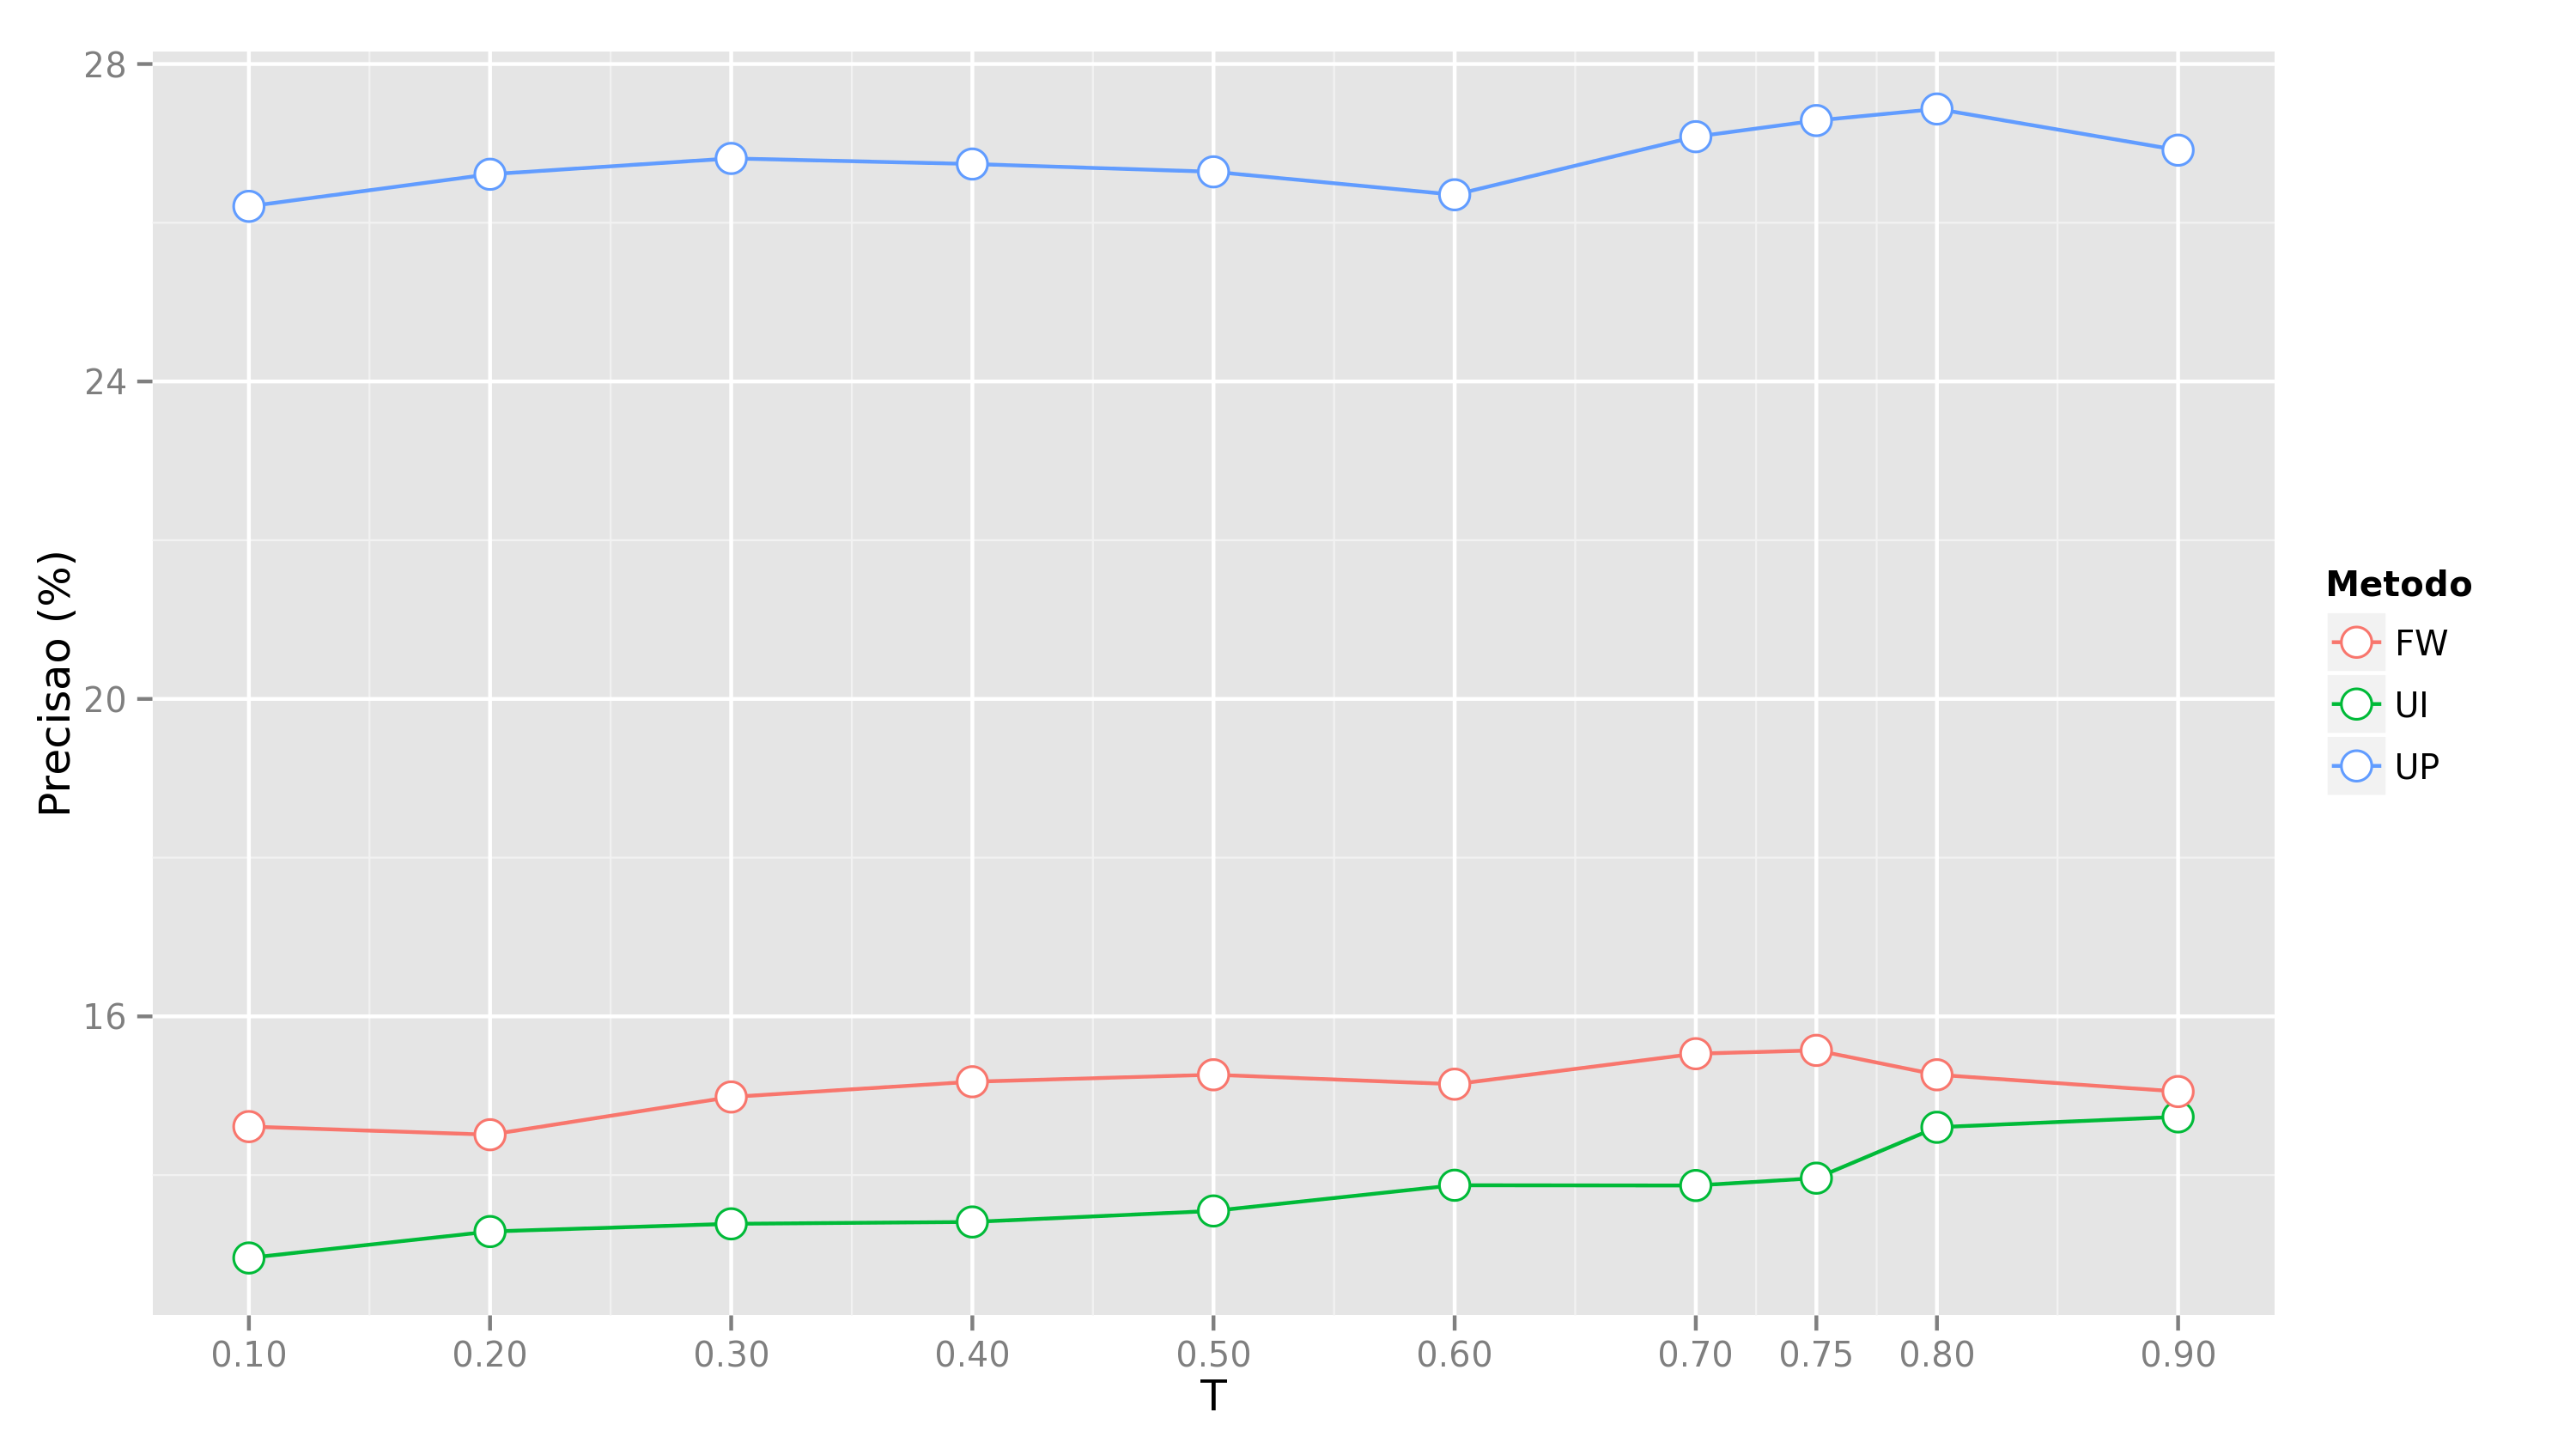
\includegraphics[width=.8\textwidth]{../img/precision_T}
    \end{center}
    \caption{Precisão $\times$ $T$}
    \label{fig:precision_T}
\end{figure}
\begin{center}
    Abrangência, $F_1$ e Tempo praticamente constantes
\end{center}
\end{frame}

\begin{frame}{Resultados}{Percentual de avaliações ``escondidas'' dos usuários-teste $H$}
\begin{figure}[ht]
    \begin{center}
    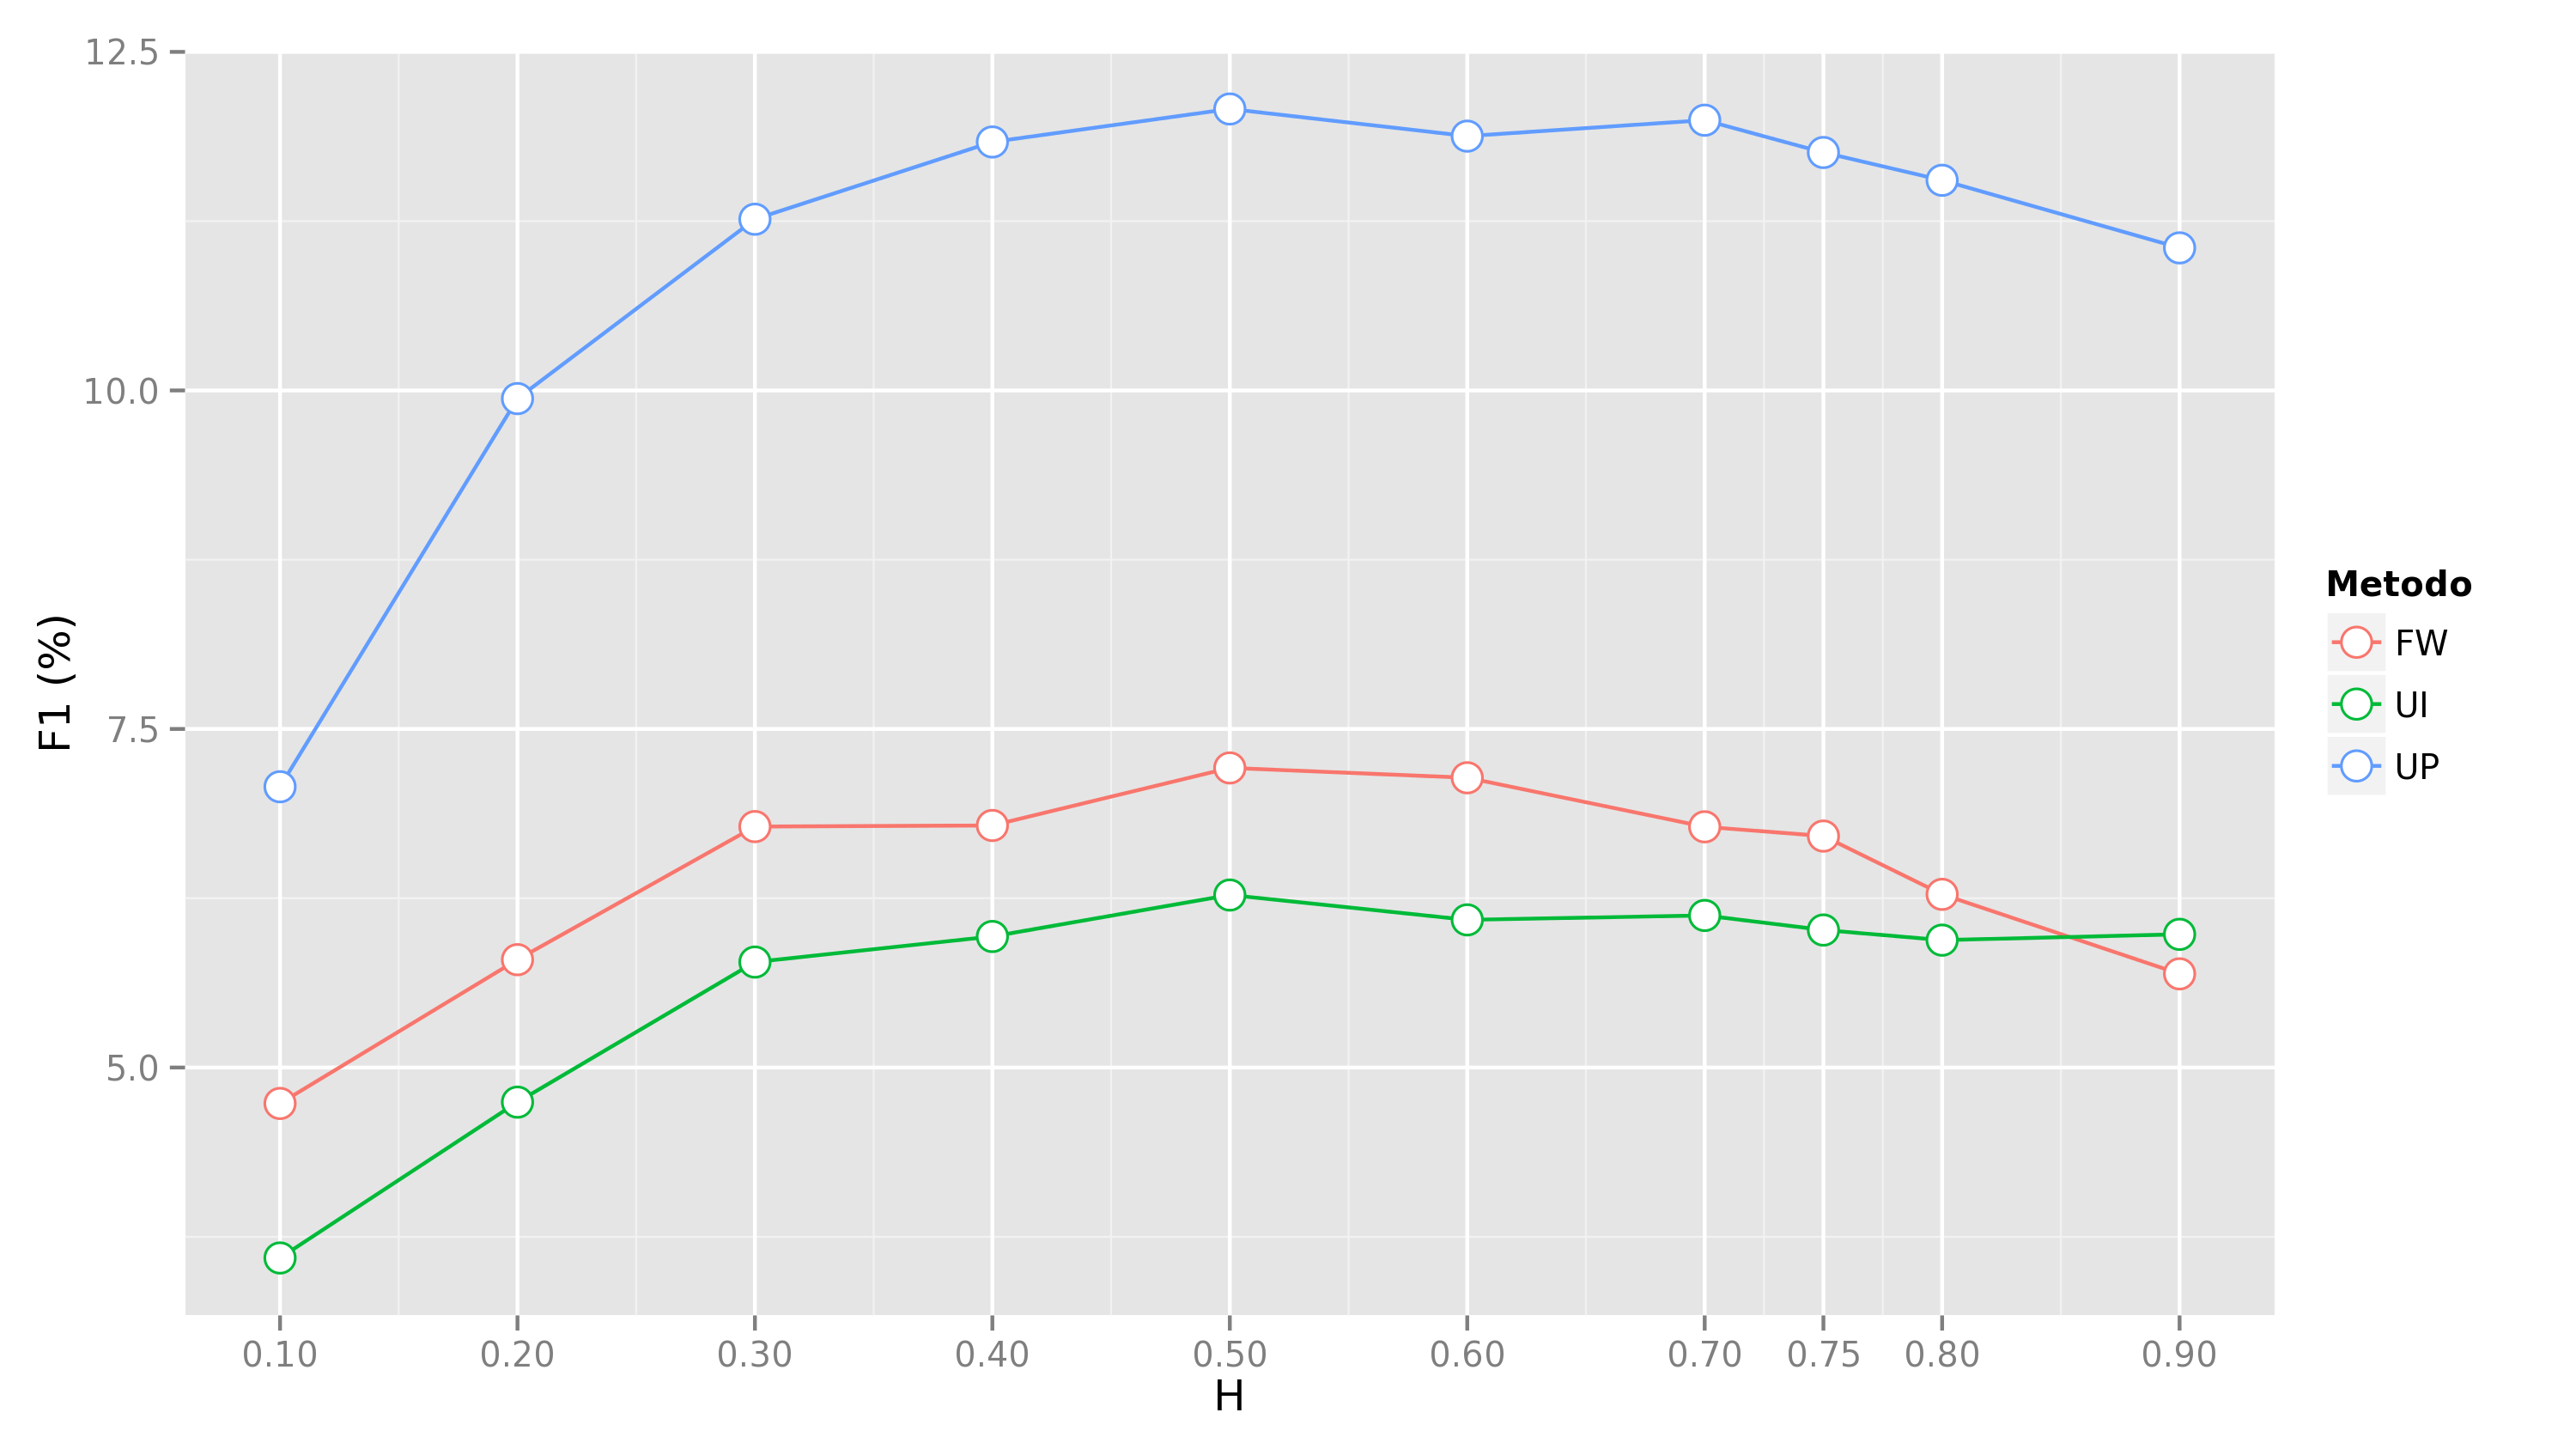
\includegraphics[width=.8\textwidth]{../img/F1_H}
    \end{center}
    \caption{$F_1$ $\times$ $H$}
    \label{fig:F1_H}
\end{figure}
\begin{center}
    Precisão cresce e Abrangência decresce
\end{center}
\end{frame}


\begin{frame}{Resultados}{Medida de distância entre atributos $d^f$}
\begin{figure}[ht]
    \begin{center}
    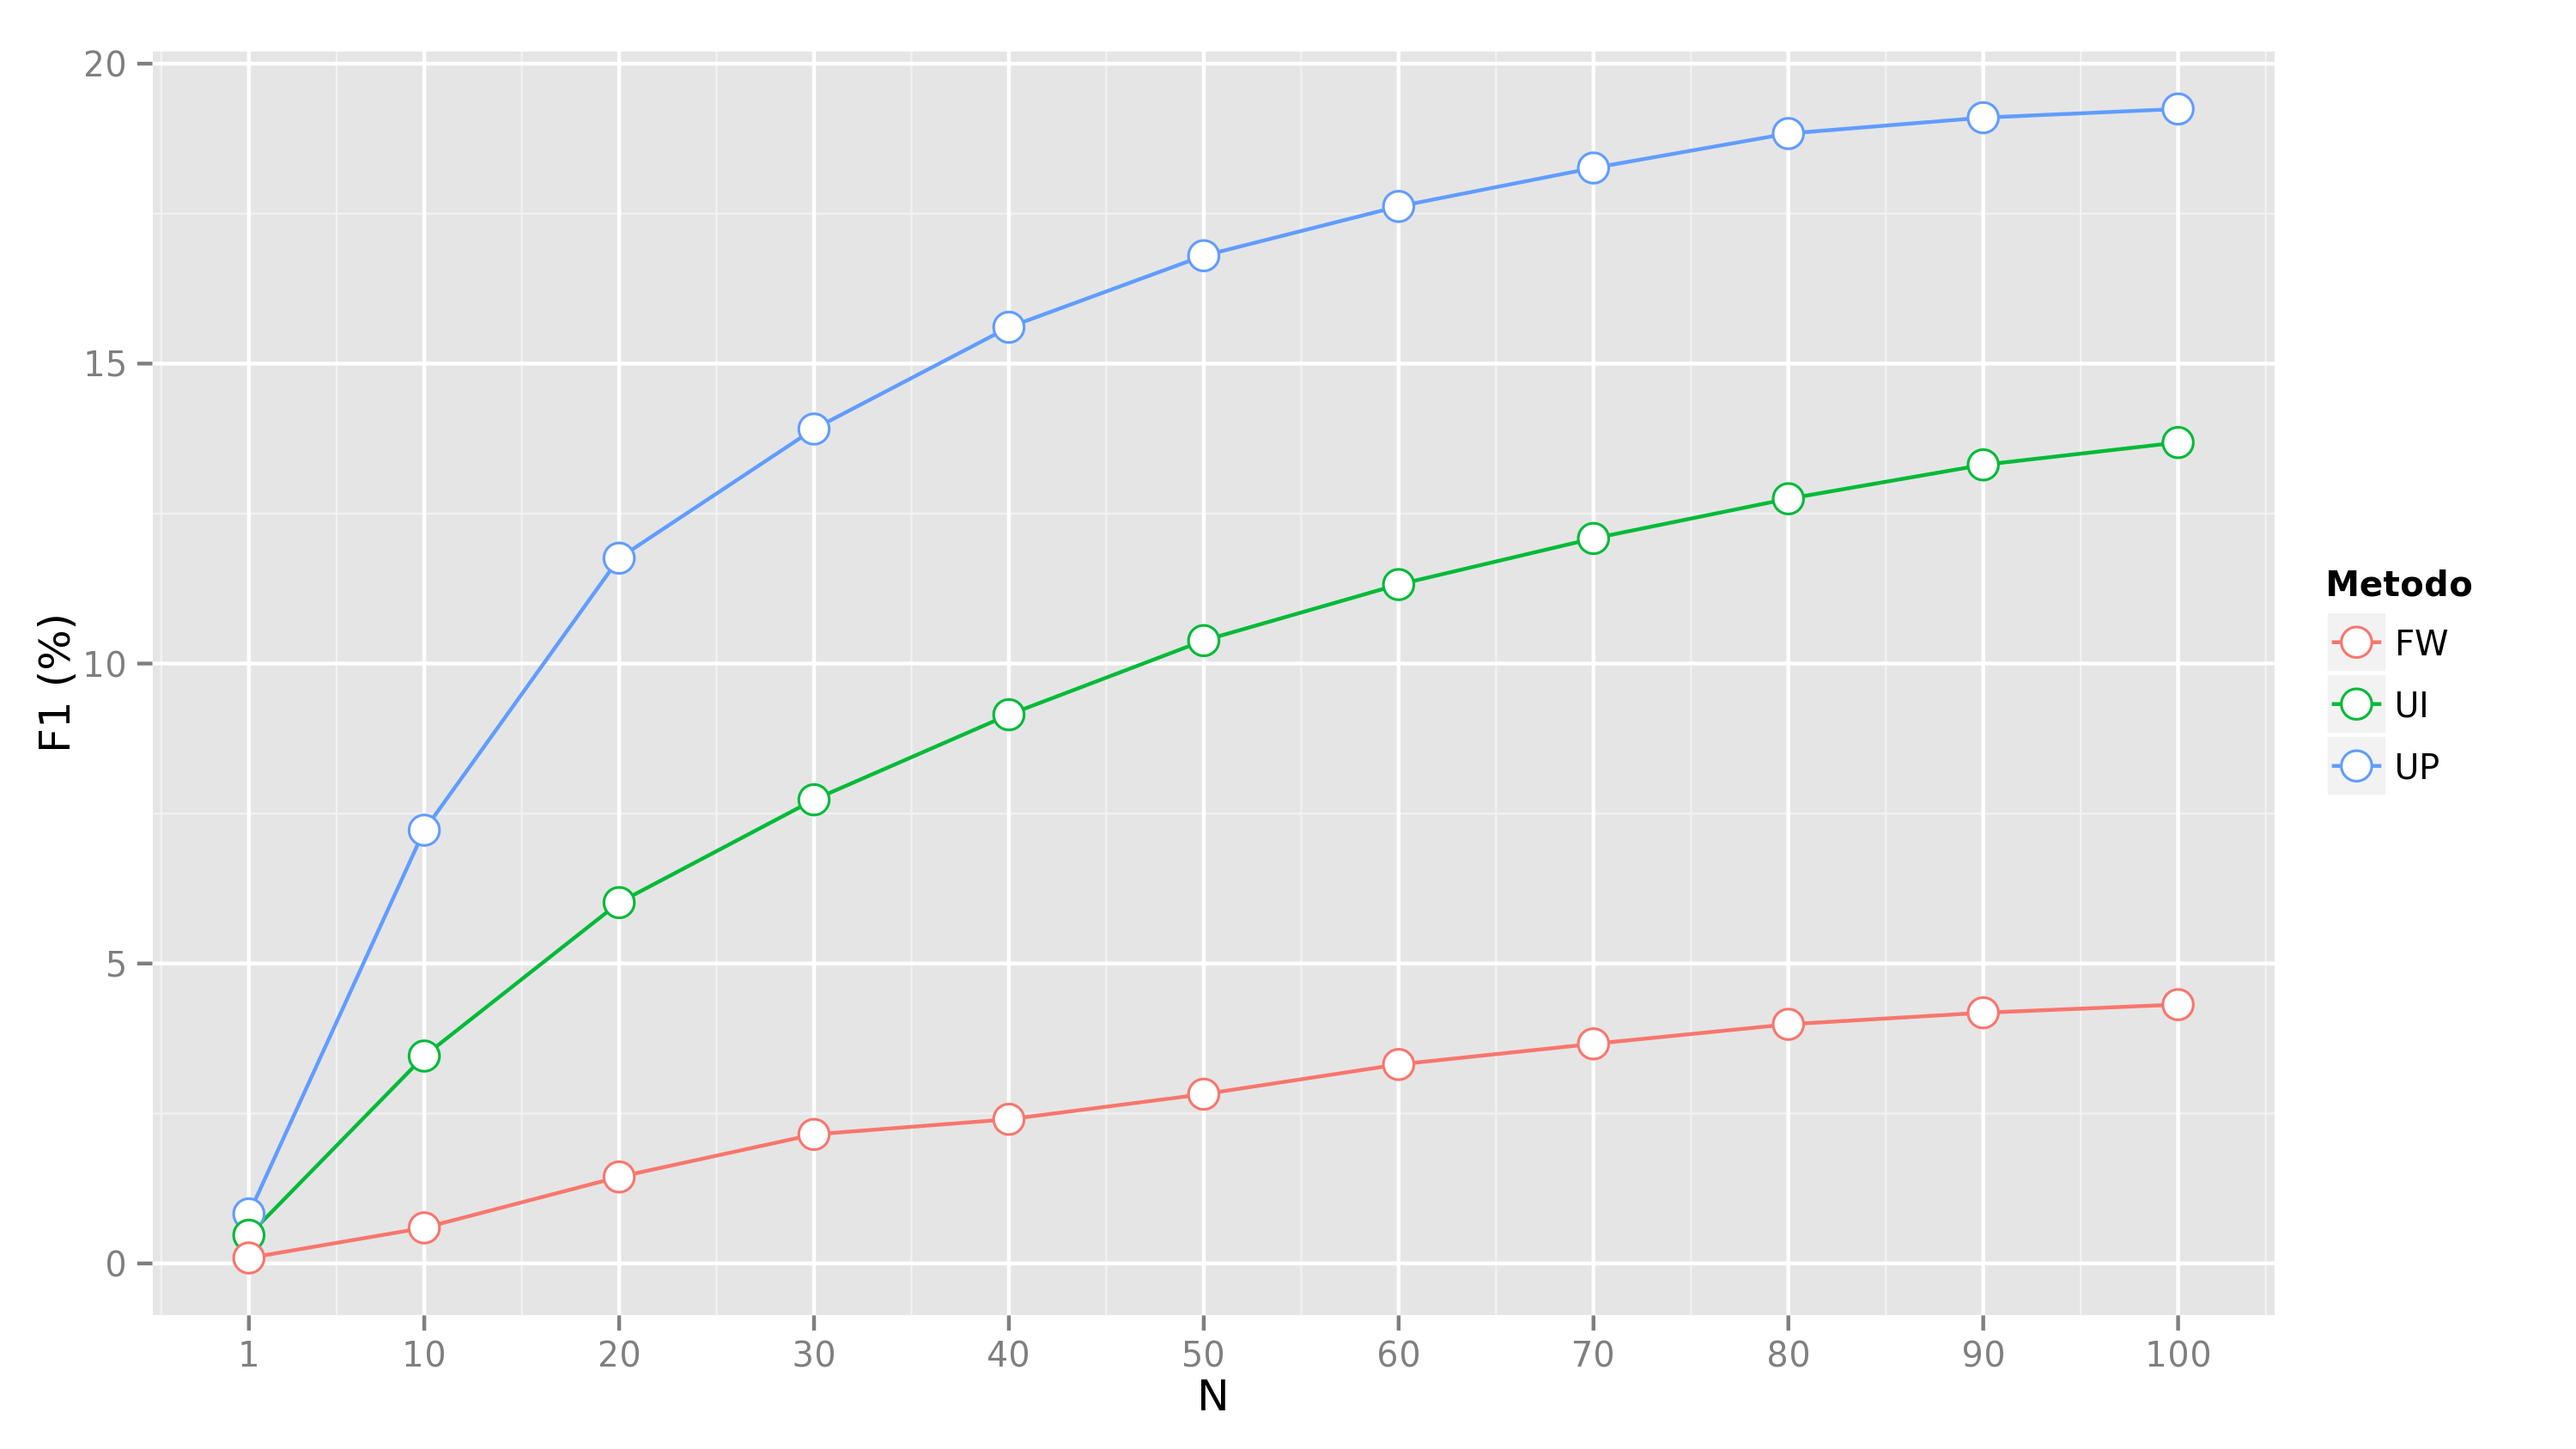
\includegraphics[width=.8\textwidth]{../img/F1_N_d}
    \end{center}
    \caption{$F_1$ $\times$ diferentes $d^f$}
    \label{fig:F1_N_d}
\end{figure}
\begin{center}
    Precisão e Abrangência diminuem com $d^f=J(A,B) ={{|A \cap B|}\over{|A \cup B|}}$
\end{center}
\end{frame}

\begin{frame}{Resultados}{Conjunto de atributos dos itens  $\mathcal{F}$}
\begin{figure}[ht]
    \begin{center}
    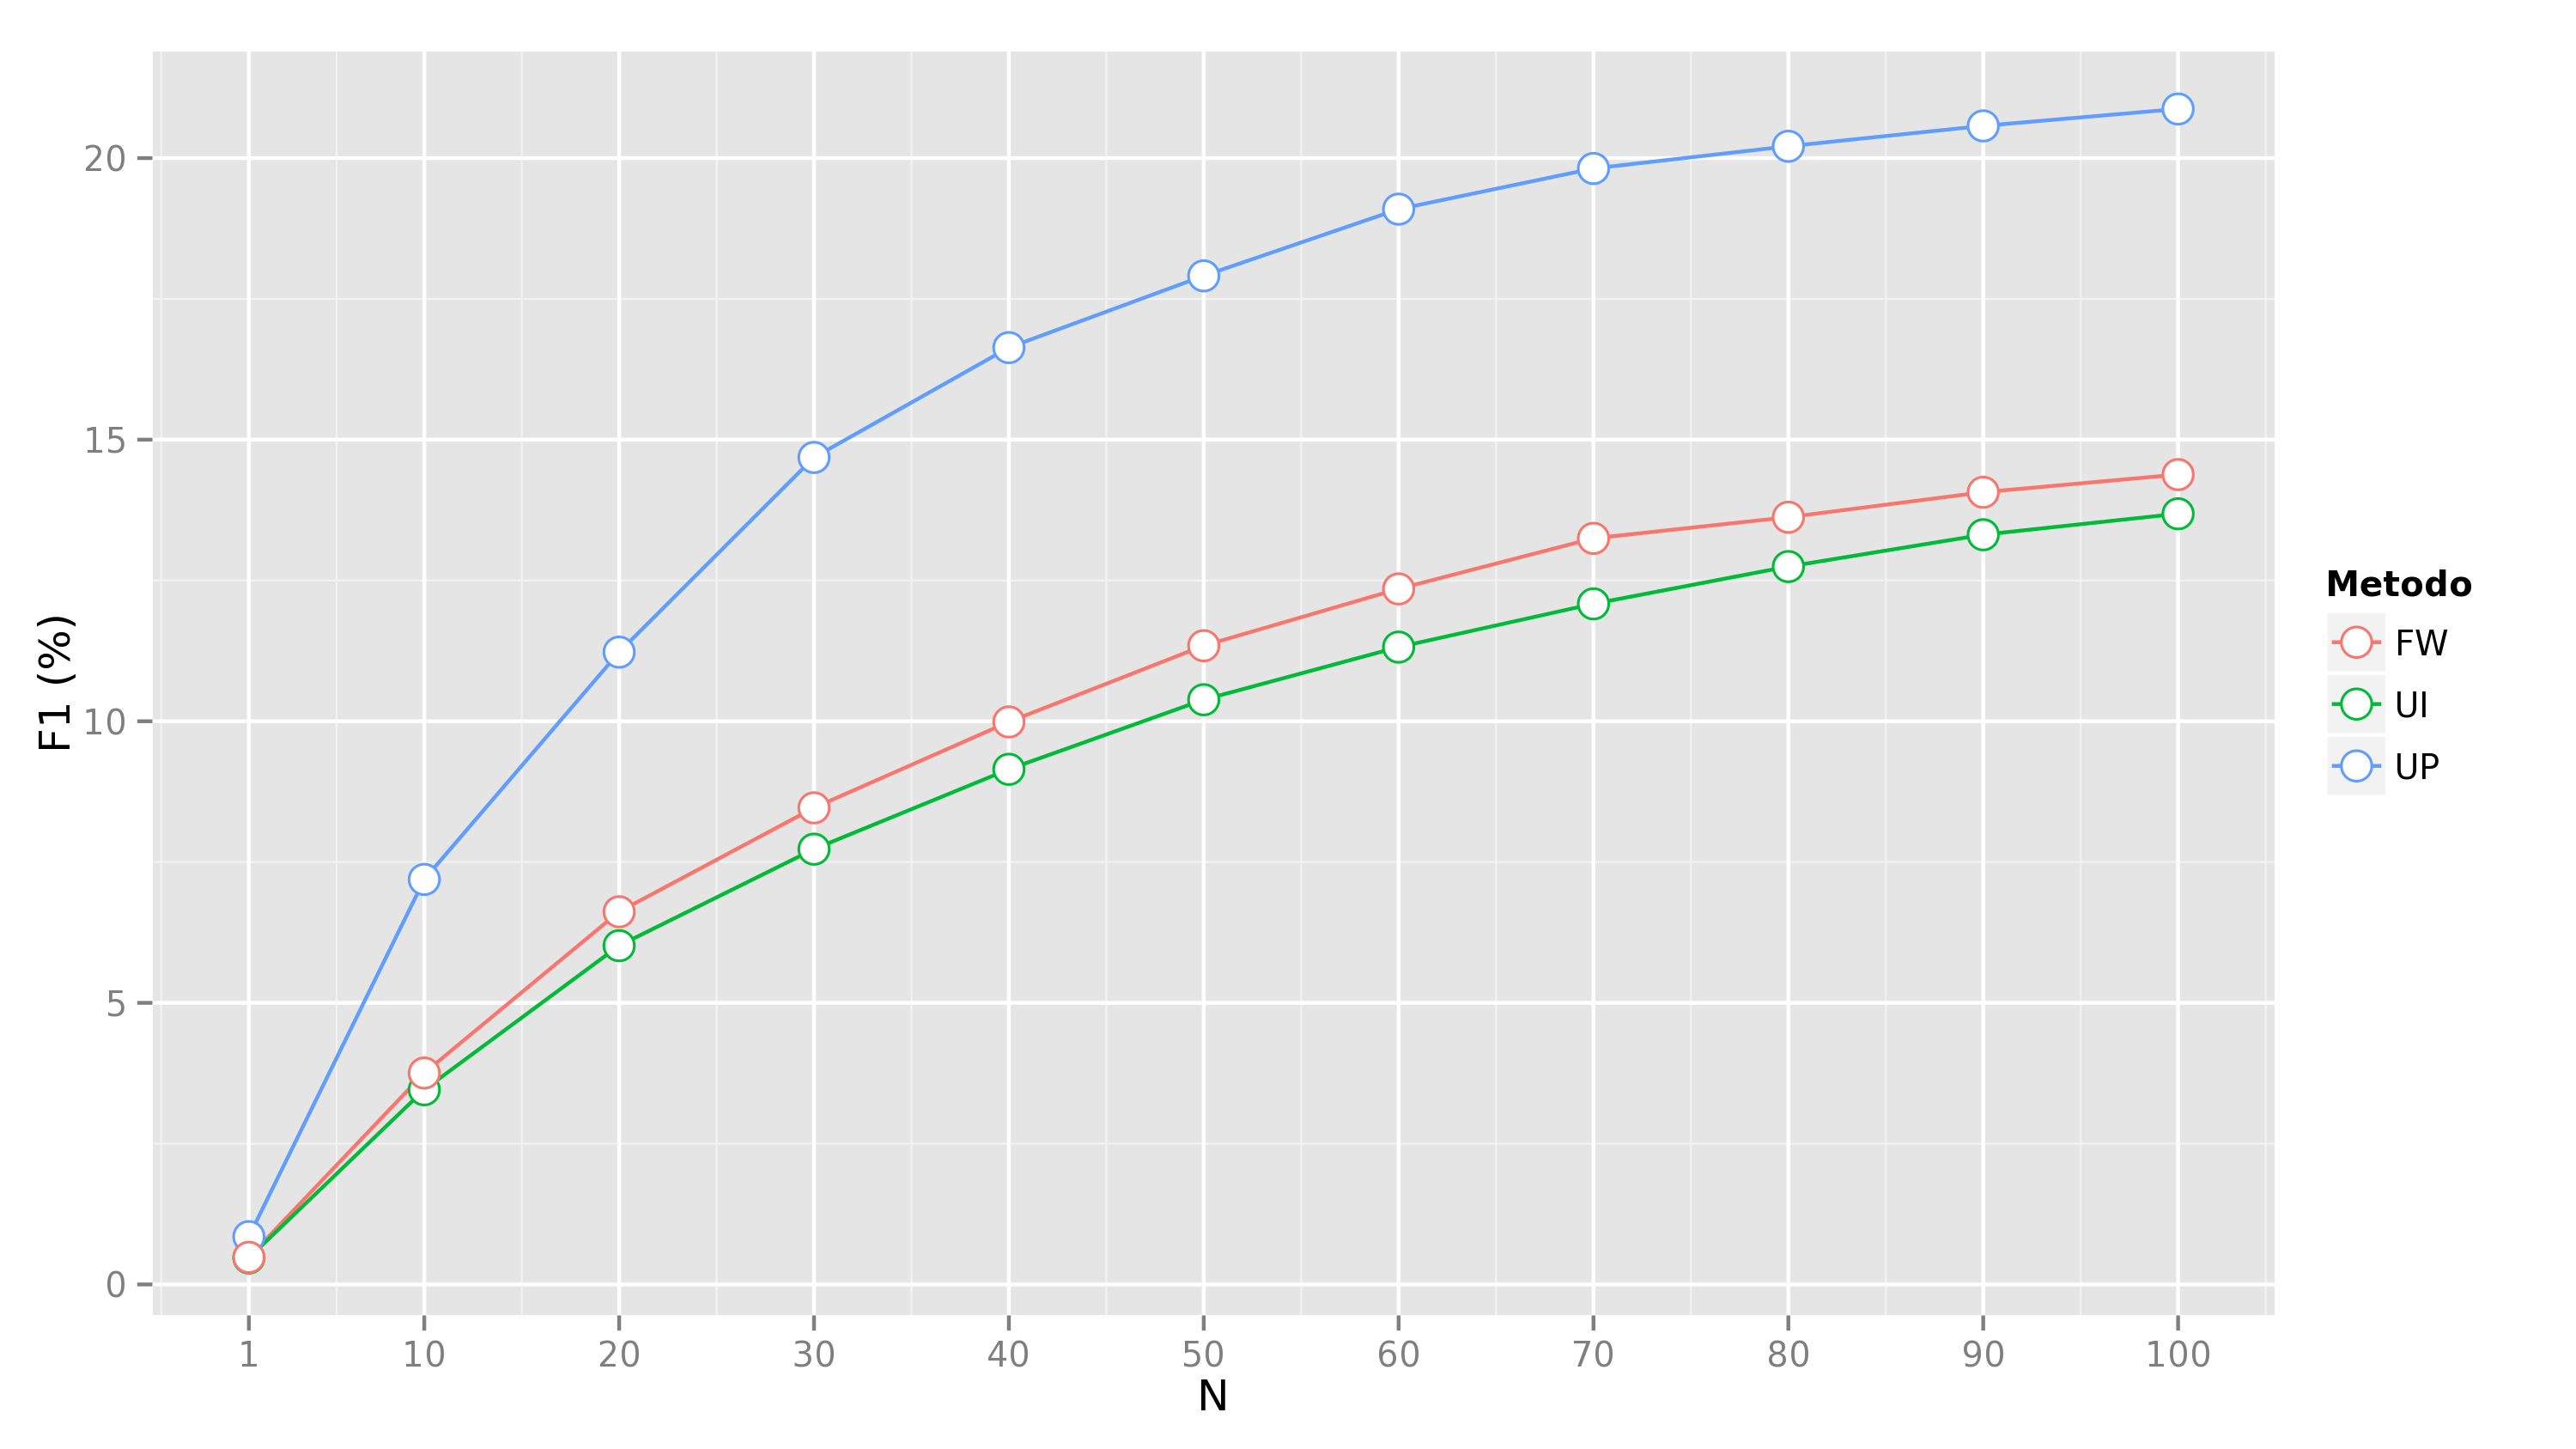
\includegraphics[width=.8\textwidth]{../img/F1_N_F}
    \end{center}
    \caption{$F_1$ $\times$ $\mathcal{F}$}
    \label{fig:F1_N_F}
\end{figure}
\begin{center}
    Precisão e Abrangência aumentam com remoção dos atributos \{data de lançamento, ano\}
\end{center}
\end{frame}




\begin{frame}{Resultados}{$M$, $k$, $W$}
\begin{columns}[b]
\column{.333\textwidth} %
\begin{figure}[ht]
    \begin{center}
    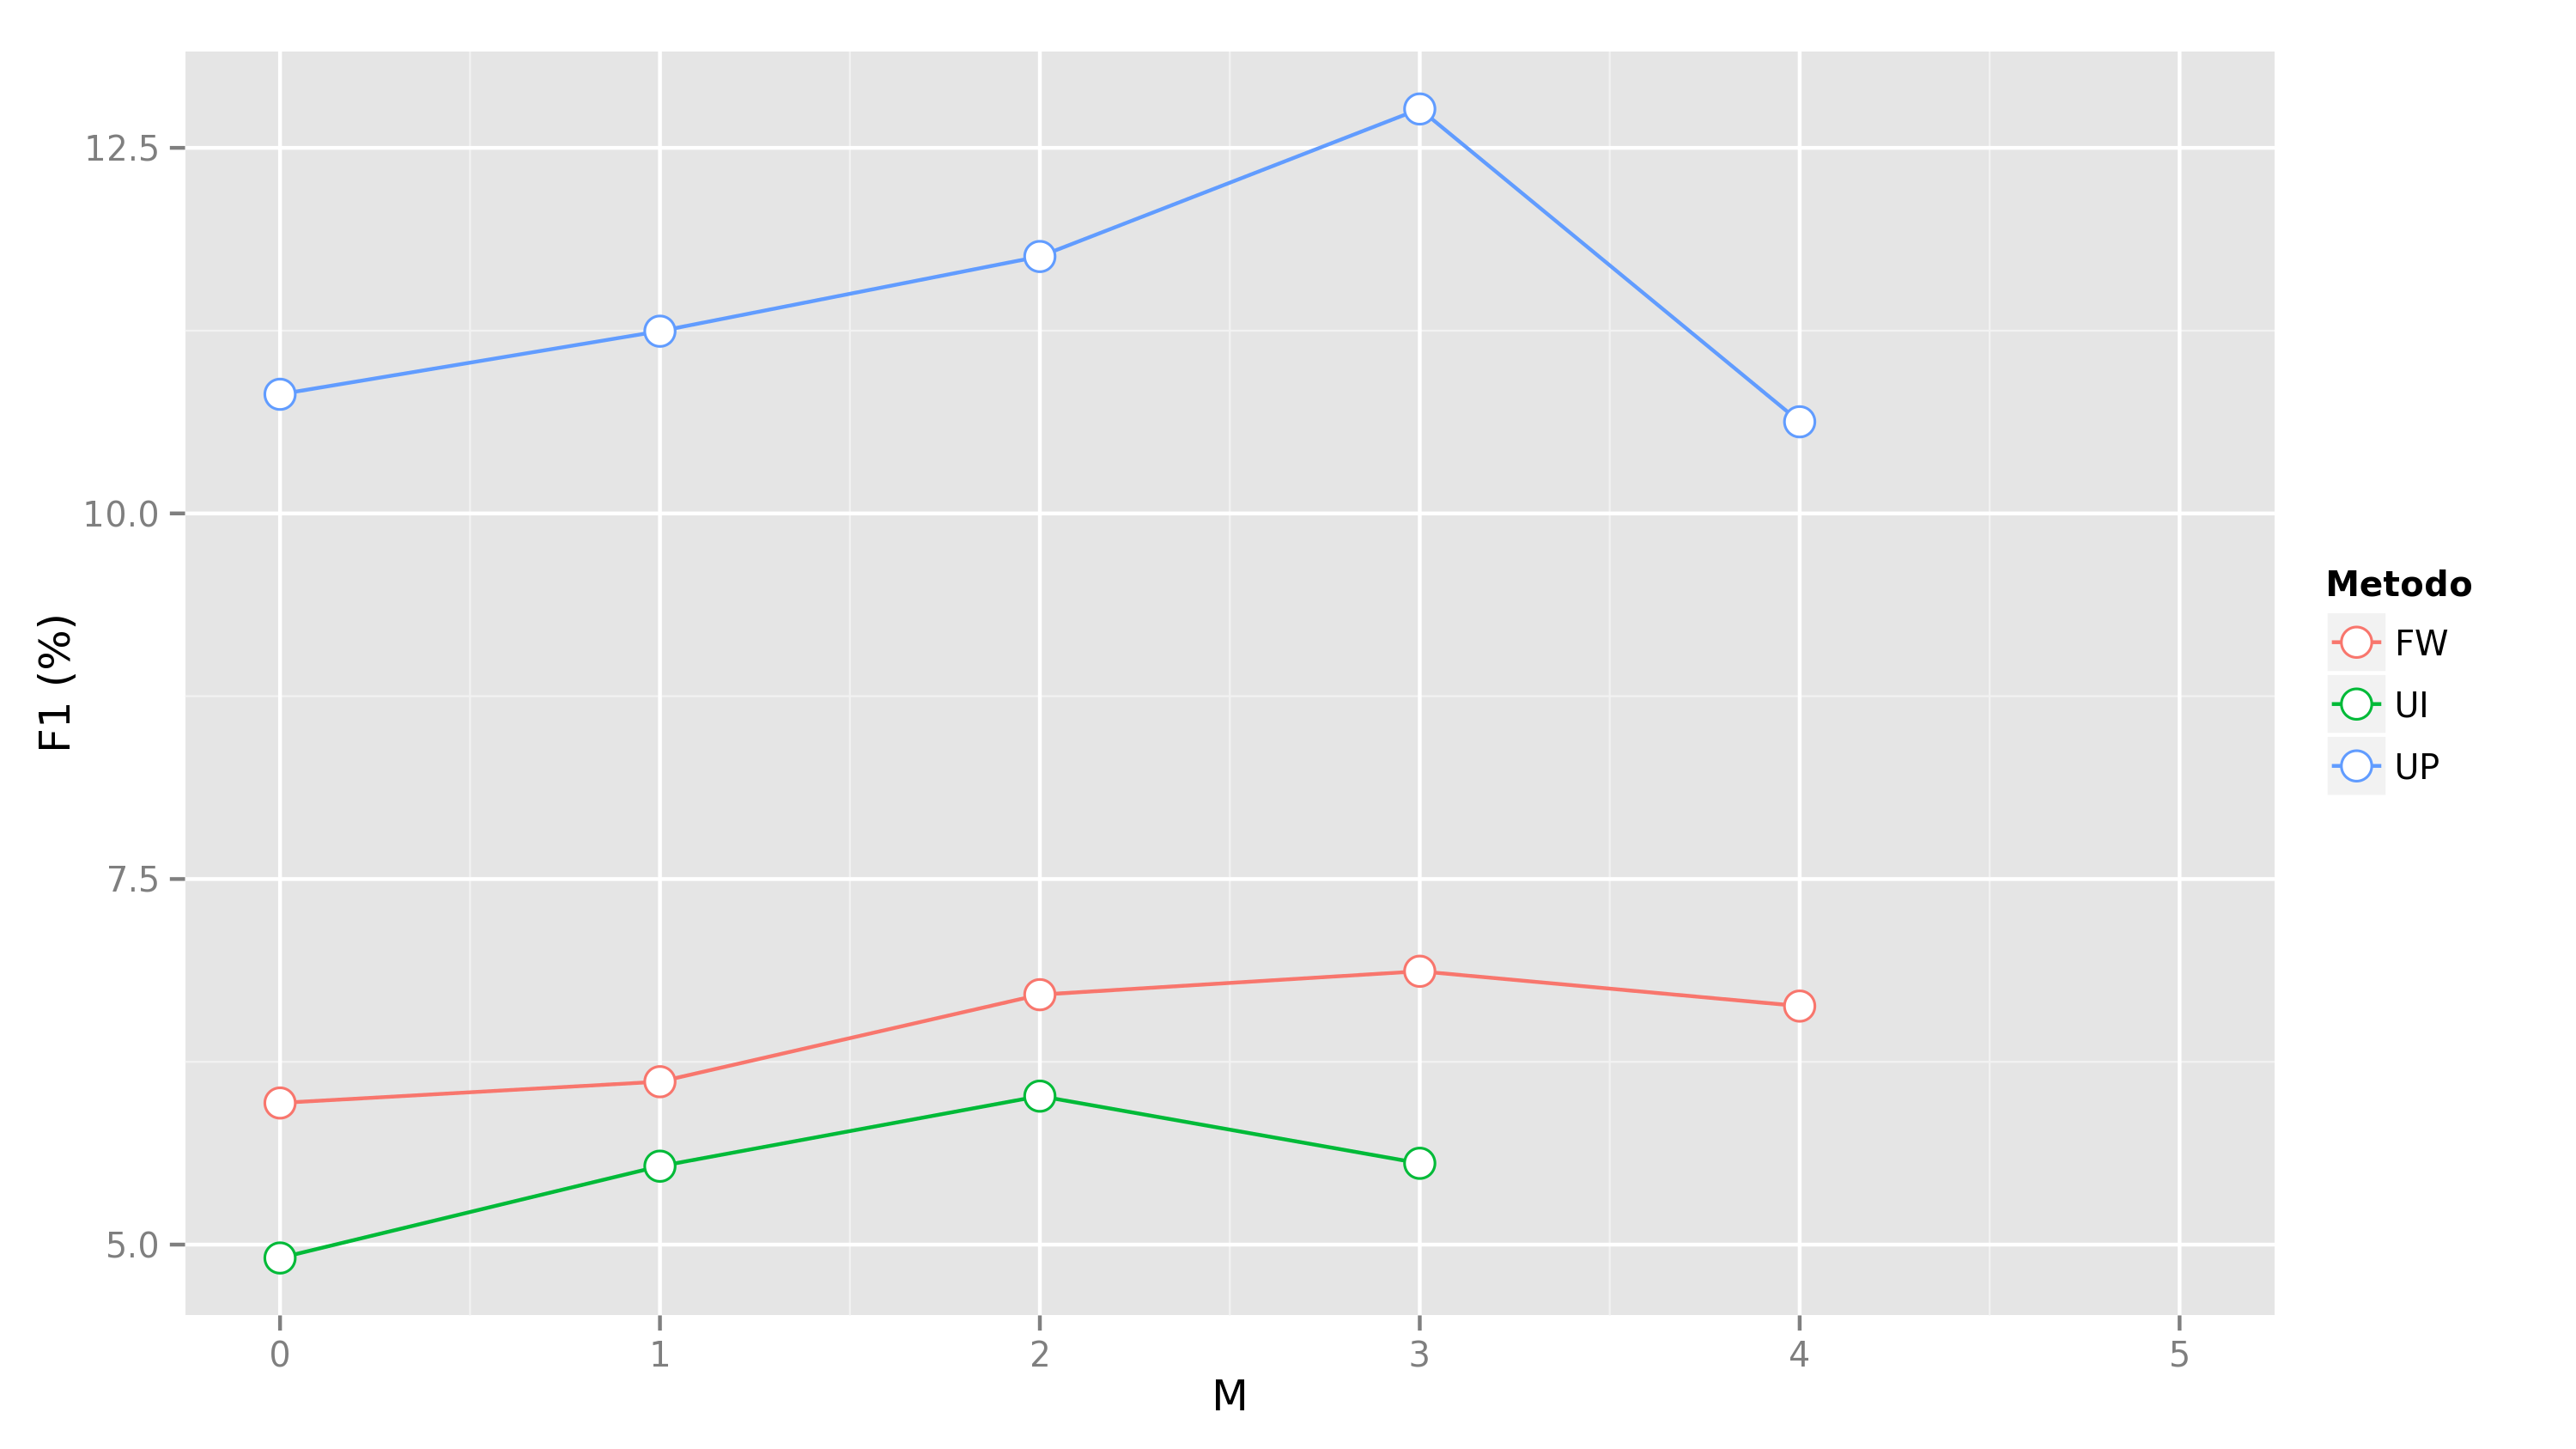
\includegraphics[width=1.1\textwidth]{../img/F1_M}
    \end{center}
    \caption{$F_1$ $\times$ $M$}
    \label{fig:F1_M}
\end{figure}

%Número de vizinhos mais próximos $k$
\column{.333\textwidth} % 
\begin{figure}[ht]
    \begin{center}
    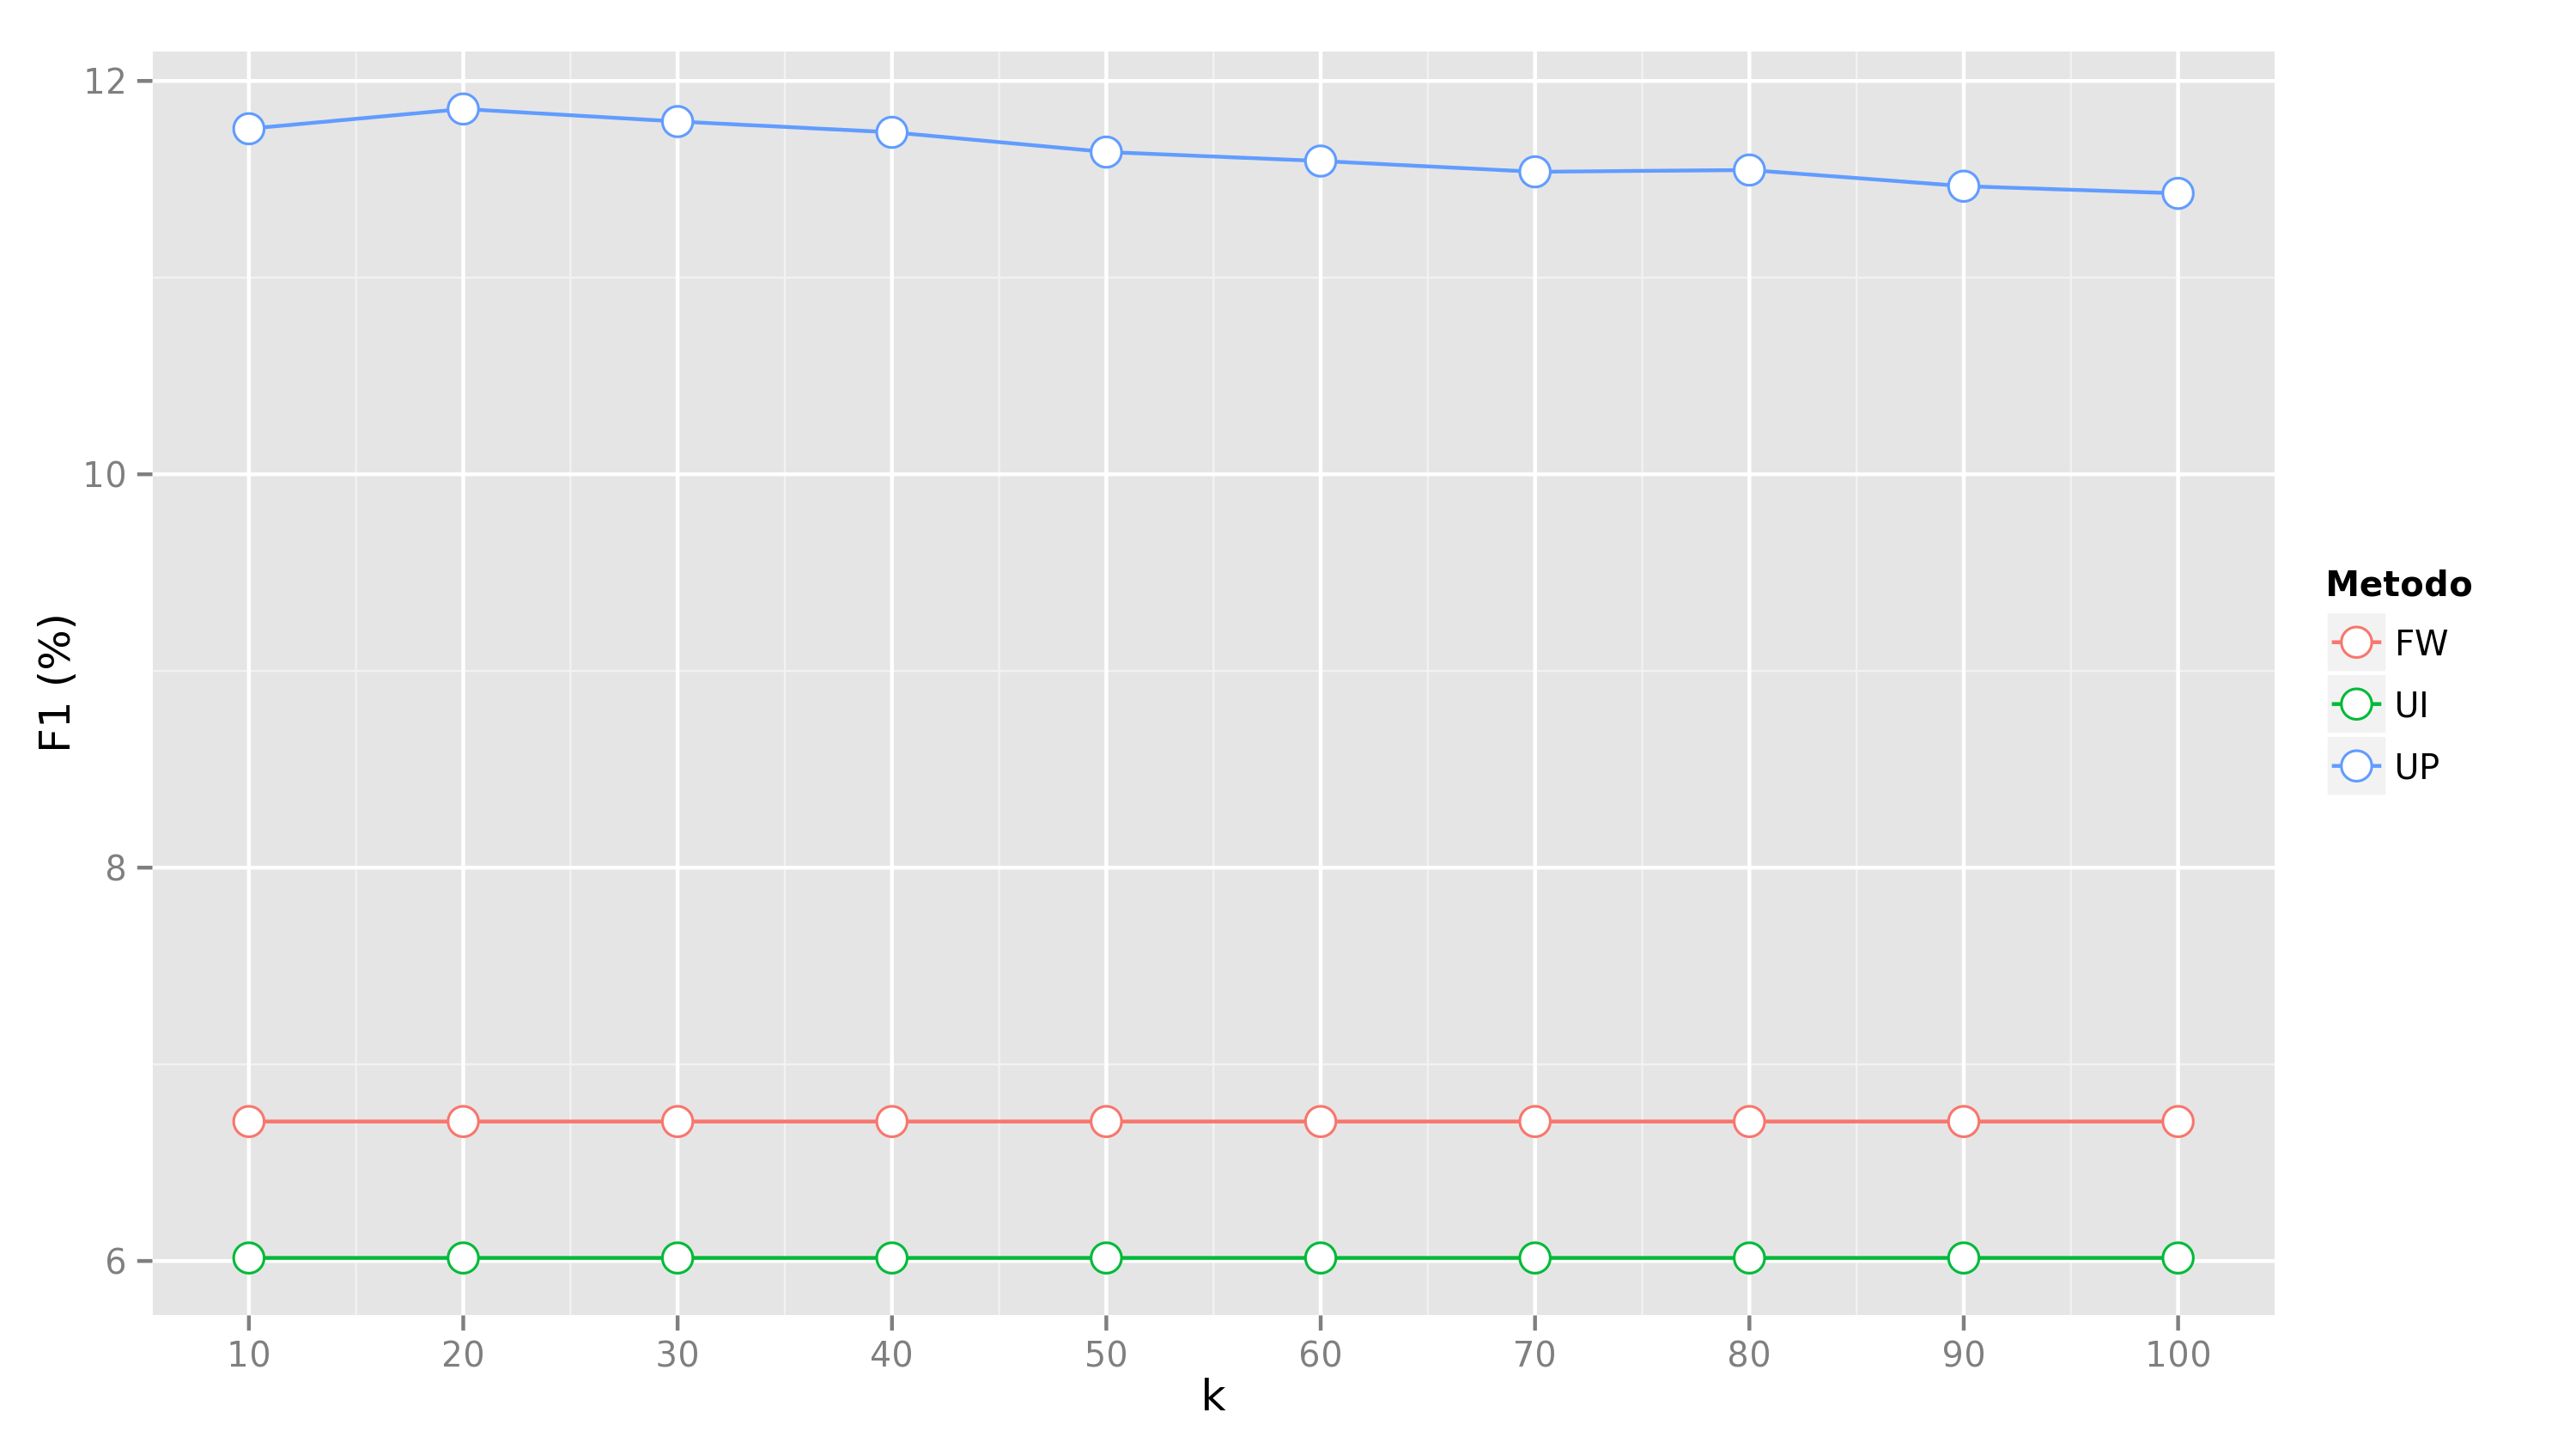
\includegraphics[width=1.1\textwidth]{../img/F1_k}
    \end{center}
    \caption{$F_1$ $\times$ $k$}
    \label{fig:F1_H}
\end{figure}
\column{.333\textwidth} % 

\begin{figure}[ht]
    \begin{center}
    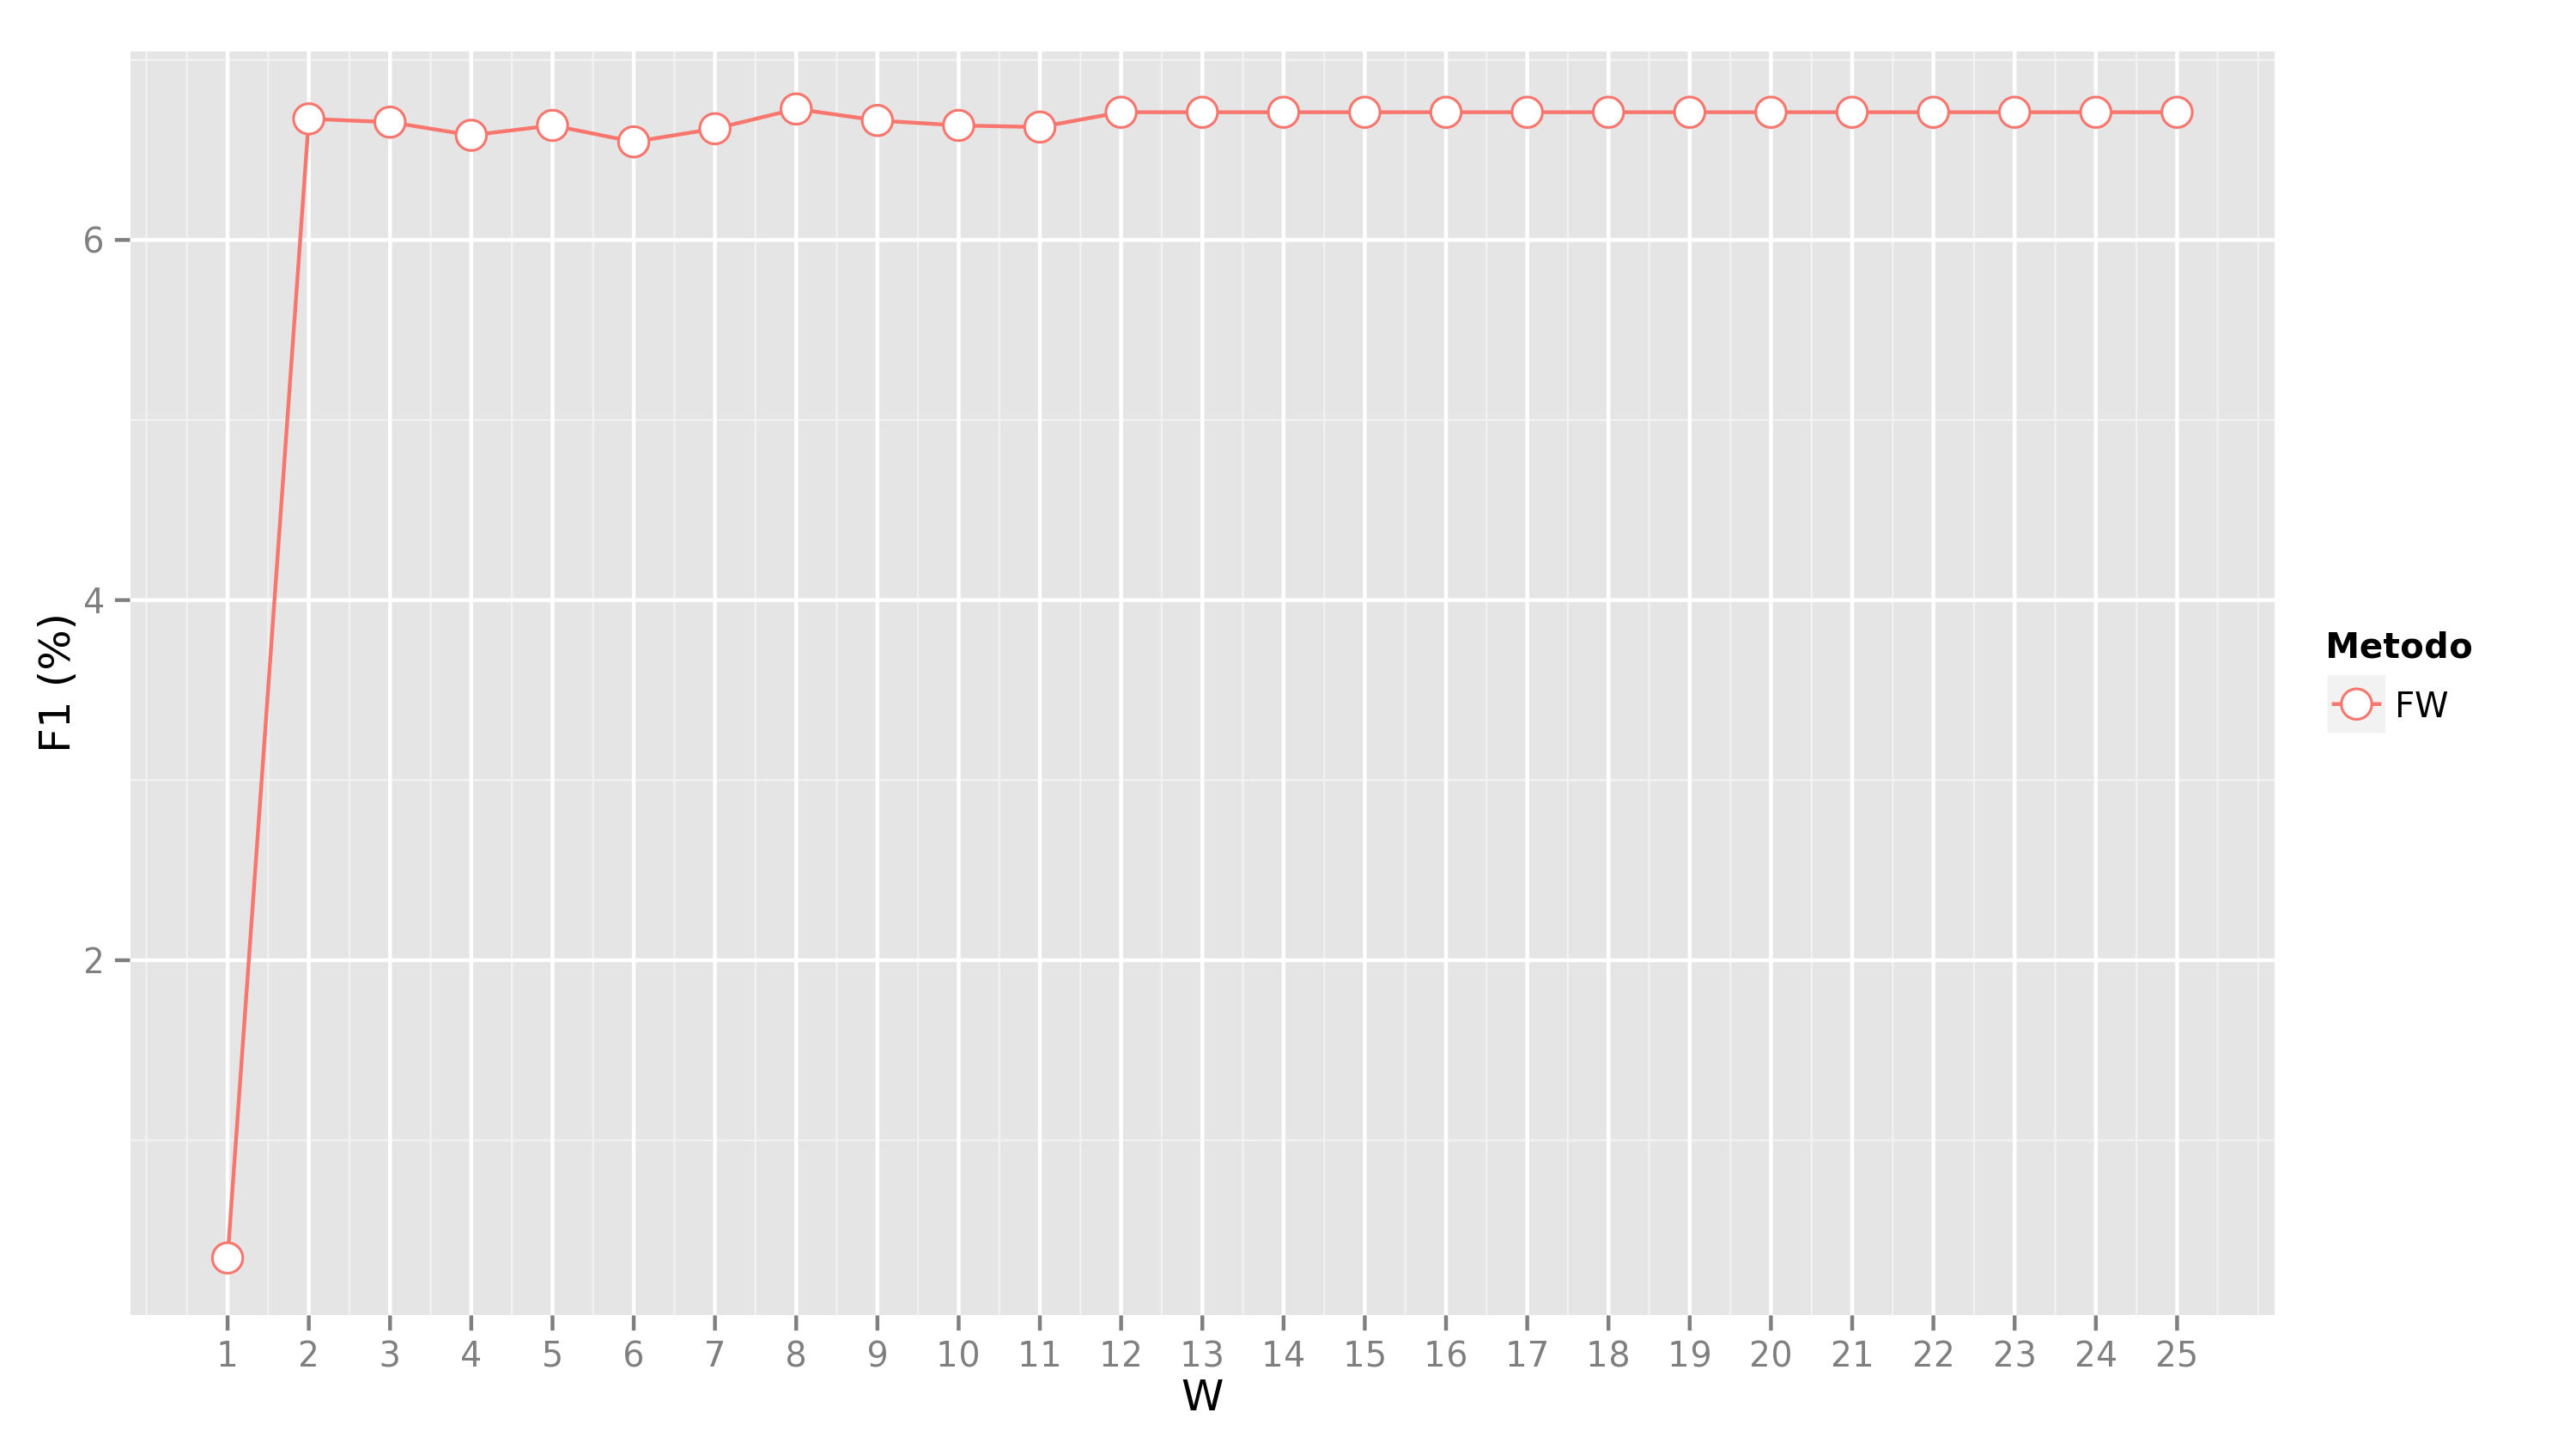
\includegraphics[width=1.1\textwidth]{../img/F1_W}
    \end{center}
    \caption{$F_1$ $\times$ $W$}
    \label{fig:F1_W}
\end{figure}
\end{columns}
\begin{center}
    Precisão e Abrangência praticamente constantes
\end{center}
\end{frame}



%\begin{figure}[ht]
%    \begin{center}
    %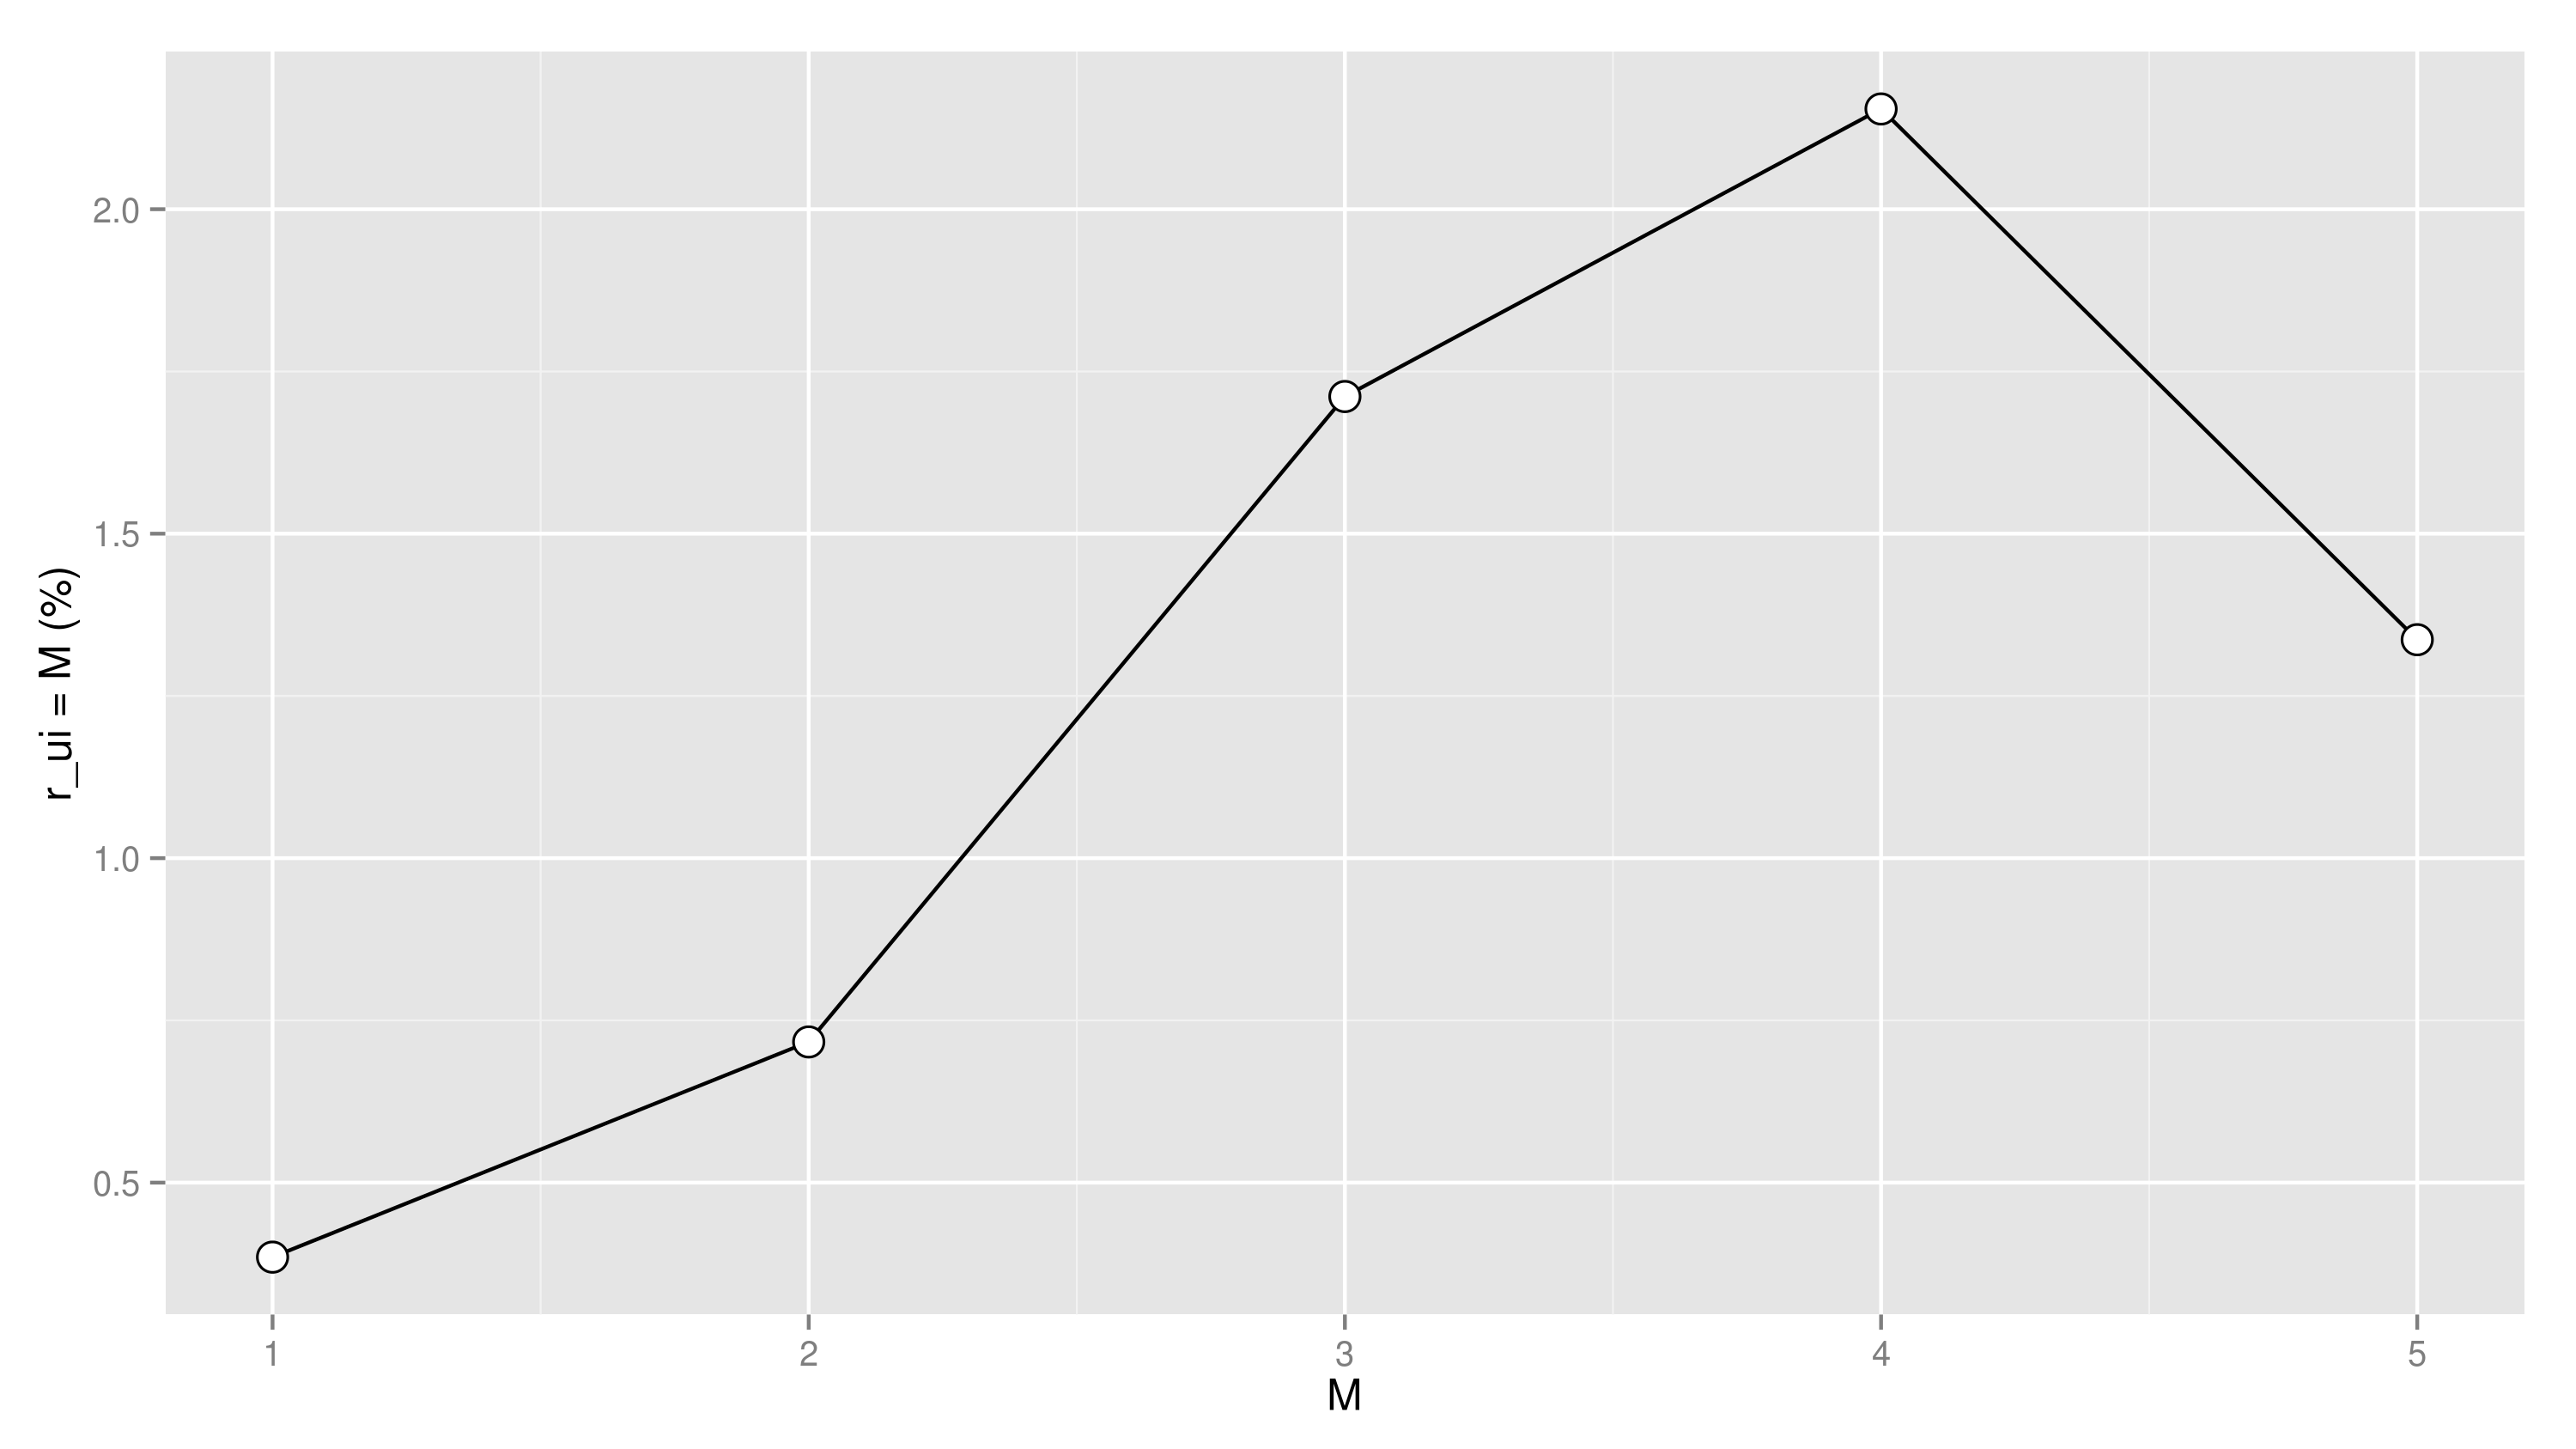
\includegraphics[width=1.1\textwidth]{../img/percentual_M}
%    \end{center}
%    \caption{\{\% $r_{ui} = M$\} $\times$ $M$}
%    \label{fig:percentual_M}
%\end{figure}

%!TEX root = index.tex
\section[Conclusão]{Conclusão}
\begin{frame}{Conclusão}
\textbf{Discussão}
\begin{itemize}
	\item Dependência entre qualidade de recomendação e $N$
	\item Mais avaliações $H$ é melhor que mais usuários $T$
	\item Muita influência de $d^f$, $\mathcal{F}$
	\item Pouca influência de $k$, $M$, $W$
\end{itemize}
\vspace{.5cm}
\textbf{Trabalhos futuros}
\begin{itemize}
	\item ``Sistema de Recomendação nas Nuvens''
	\item Eliminação de restrições de entrada/saída de dados
	\item Desenvolvimento de um \textit{driver} SQL 
	\item Reconstrução da biblioteca em C
	\item Aplicação em um banco de dados de um e-commerce real
\end{itemize}
\end{frame}
%%!TEX root = index.tex
\chapter[Cronograma]{Cronograma}
\label{chap:cronograma}

O cronograma de atividades da dupla busca seguir o cronograma proposto pela banca avaliadora dos trabalhos de conclusão de curso, estando sempre à frente das entregas em pelo menos uma semana. Dessa maneira, é possível apresentar a entrega antecipadamente ao orientador e falar sobre possíveis mudanças ou correções.

Além disso, semanalmente os alunos se reunem com o orientador a fim de conversar sobre o andamento do projeto, apresentar-lhe o esboço dos relatórios e discutir a implementação dos algoritmos. 

Para o segundo semestre, trabalharemos na implementação do sistema de recomendação já no período de férias escolares, para poder ter uma amostra funcional no início das aulas. Em seguida, daremos início ao relatório final em paralelo com os testes de performance do sistema de recomendação, e esperamos finalizar o projeto dentro do prazo estipulado.

O cronograma detalhado da dupla está descrito a seguir:

\begin{description}
	\item[09/07] Pré-tratamento do banco de dados
 	\item[16/07] Programação do método \textit{FW} e variantes, descritos no relatório final
 	\item[23/07] Programação do método \textit{UP} e variantes, descritos no relatório final
 	\item[30/07] Análise comparativa dos dois algoritmos
 	\item[13/08] Relatório de atividades de implementação
 	\item[27/08] Primeiros testes com o sistema (precisão e acurácia para uma base de testes)
 	\item[03/09] Testes com o sistema (validação cruzada)
 	\item[24/09] Melhorias incrementais e relatório de atividades
 	\item[15/10] Relatório aprofundado de atividades
 	\item[05/11] Elaboração da apresentação e finalização dos relatórios
 	\item[12/11] Melhorias incrementais
 \end{description} 

\appendix
%!TEX root = index.tex
{\unnumbered
\begin{frame}[allowframebreaks]{Bibliografia}
\bibliography{../bibliografia}
\end{frame}}

\end{document} 
